\documentclass{report}

\usepackage{amsmath, amsthm, amssymb, amsfonts}
\usepackage{thmtools}
\usepackage{graphicx}
\usepackage{setspace}
\usepackage[margin=3cm]{geometry}
\usepackage{float}
\usepackage{hyperref}
\usepackage[utf8]{inputenc}
\usepackage[english]{babel}
\usepackage{framed}
\usepackage[dvipsnames]{xcolor}
\usepackage{tcolorbox}
\usepackage{parskip}
\usepackage{subcaption}

\colorlet{LightGray}{White!90!Periwinkle}
\colorlet{LightOrange}{Orange!15}
\colorlet{LightGreen}{Green!15}

\newcommand{\HRule}[1]{\rule{\linewidth}{#1}}
\newcommand{\indep}{\perp \!\!\! \perp}

\DeclareMathOperator*{\argmax}{arg\,max}
\DeclareMathOperator*{\argmin}{arg\,min}

\declaretheoremstyle[name=Theorem,]{thmsty}
\declaretheorem[style=thmsty,numberwithin=section]{theorem}
\tcolorboxenvironment{theorem}{colback=LightGray}

\declaretheoremstyle[name=Proposition,]{prosty}
\declaretheorem[style=prosty,numberlike=theorem]{proposition}
\tcolorboxenvironment{proposition}{colback=LightOrange}

\declaretheoremstyle[name=Principle,]{prcpsty}
\declaretheorem[style=prcpsty,numberlike=theorem]{principle}
\tcolorboxenvironment{principle}{colback=LightGreen}

\setstretch{1.2}
\geometry{
    textheight=9in,
    textwidth=5.5in,
    top=1in,
    headheight=12pt,
    headsep=25pt,
    footskip=30pt
}

% ------------------------------------------------------------------------------

\begin{document}

% ------------------------------------------------------------------------------
% Cover Page and ToC
% ------------------------------------------------------------------------------

\title{ \normalsize \textsc{}
		\\ [2.0cm]
		\HRule{1.5pt} \\
		\LARGE \textbf{\uppercase{AI Algorithms}
		\HRule{2.0pt} \\ [0.6cm] \LARGE{Data Science Handbook} \vspace*{10\baselineskip}}
		}
\date{}
\author{\textbf{Author} \\ 
		  Nelson Bruno Andrés Moreno Cabañas \\
		Santiago, Chile \\
		2024}

\maketitle
\newpage

\tableofcontents
\newpage

% ------------------------------------------------------------------------------

\section{Introduction}

Esta es la introducción. 
\newpage

\chapter{Basic Concepts}

\section{Performance Metrics} 

Para medir el performance de un modelo de \textit{Machine Learning} ya sea en problemas de clasificación o regresión, es posible utilizar distintas métricas de acuerdo a lo que nos importa medir en cada situación. 

\subsection{Classification Metrics}

\begin{figure}[H]
    \center
    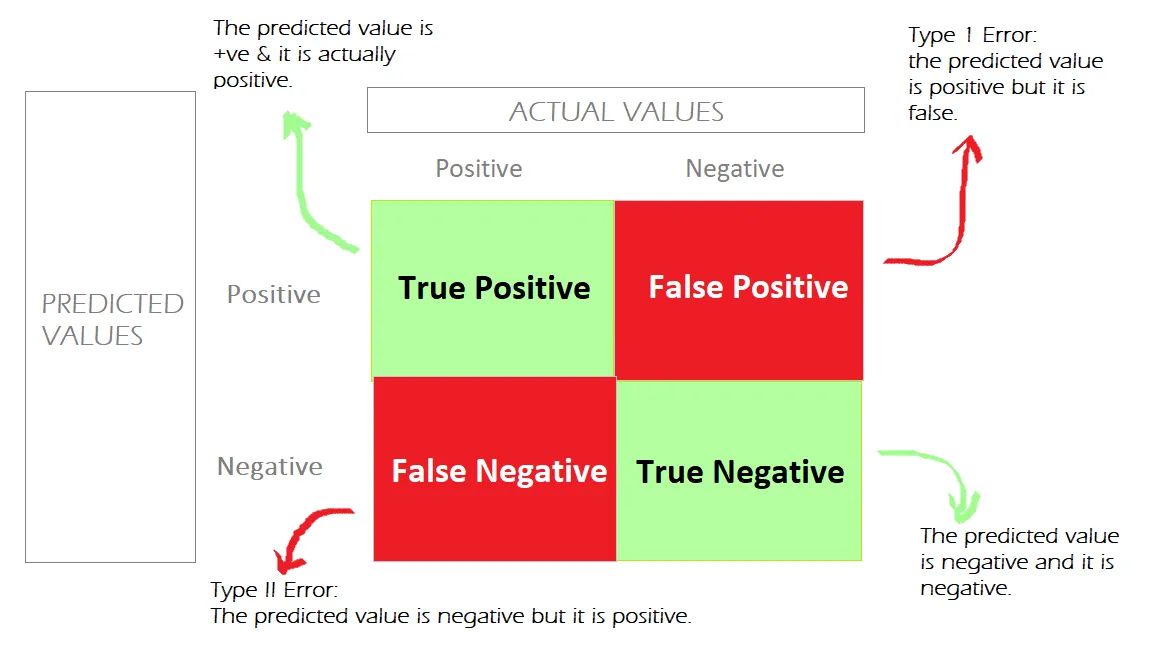
\includegraphics[scale=0.25]{notebooks/Basic/img/confusion_matrix_diagram.png}
    \caption{Confusion Matrix Diagram}
\end{figure}

En las métricas para problemas de clasificación, podemos encontrar
\begin{enumerate}
    \item \textbf{Accuracy:} Se define como el total de aciertos positivos y negativos sobre el total de predicciones. 
    $$ 
    \text{Accuracy} = \frac{TP + TN}{TP + TN + FP + FN}
    $$
    \item \textbf{Precision:} Este es el porcentaje de identificaciones positivas correctas en el total de identificaciones positivas. 
    $$
    \text{Precision} = \frac{TP}{TP + FP}
    $$
    \item \textbf{Recall: } Este es el porcentaje de identificaciones positivas correctas en el total de datos positivos. 
    $$ 
    \text{Recall} = \frac{TP}{TP + FN}
    $$
    \item \textbf{F1 - Score: } Esta métrica es la media armónica entre la precisión y el recall. 
    $$ 
    F_{1} = \frac{2}{\frac{1}{\text{precision}} + \frac{1}{\text{recall}}} = 2 \frac{\text{precision} \cdot \text{recall}}{\text{precision} + \text{recall}}
    $$
    Si alguna de las métricas tiene una mayor importancia dado el contexto del problema, podemos amplificarla por un valor $\beta$ de la siguiente forma
    $$ 
    F_{\beta} = (1 + \beta^2) \frac{\text{precision} \cdot \text{recall}}{\beta^2 \cdot \text{precision} + \text{recall}}
    $$
    Es decir, el recall es $\beta$ veces más importante que la precisión. 
\end{enumerate}

En problemas de clasificación binario, definir si un score se asigna al label positivo (1) o negativo (0) depende de un umbral (threshold) que se puede definir en base a qué métrica queremos optimizar. Lo anterior da origen a la curva \textit{Precision - Recall}

\begin{figure}[H]
    \center
    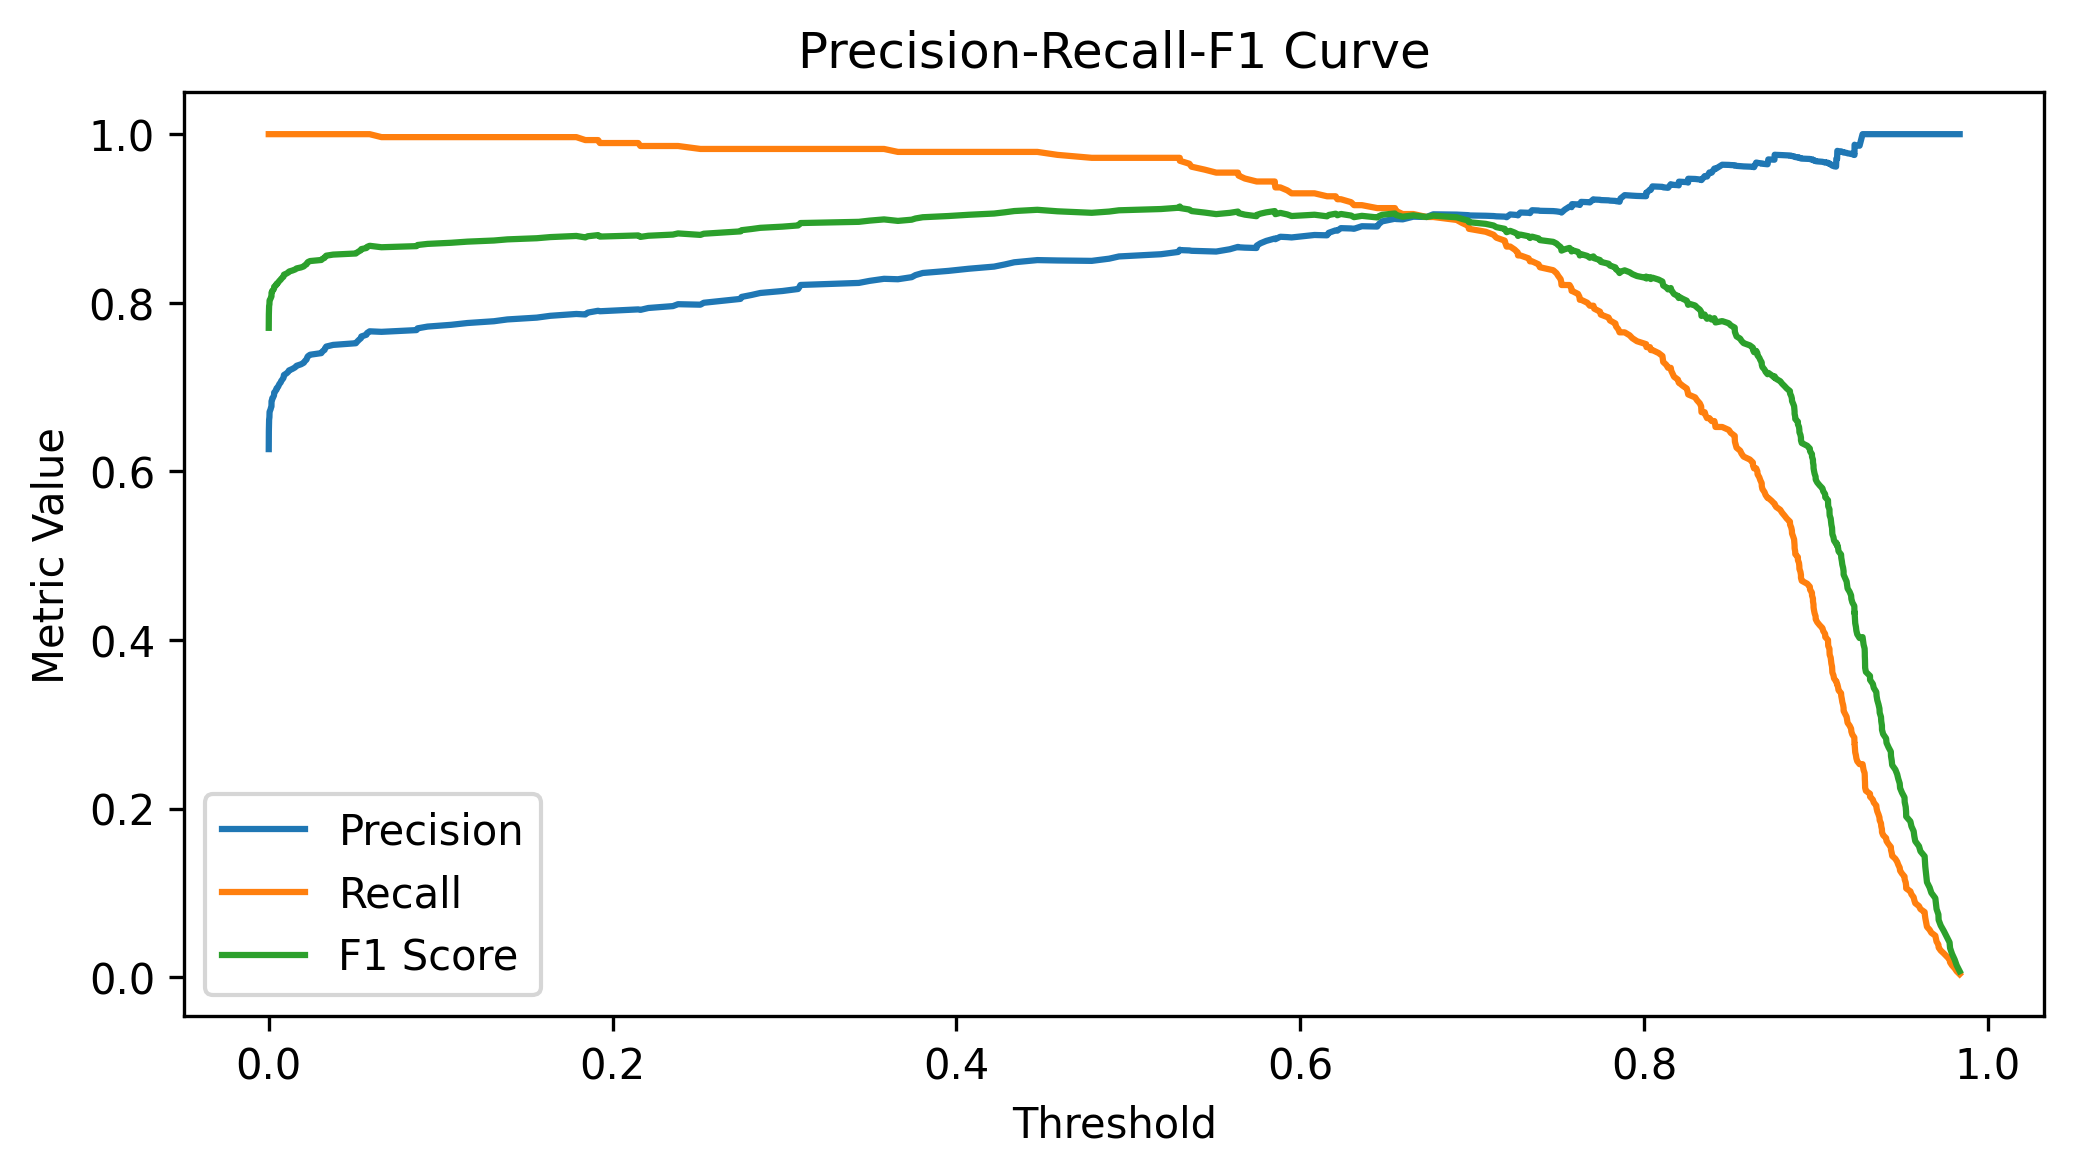
\includegraphics[scale=0.5]{notebooks/Basic/img/precision_recall_f1_curve.png}
    \caption{Precision-Recall-F1 Curve}
\end{figure}

Es fácil ver que el máximo de la métrica $F_{1}$ se alcanza en la intersección de la Precision y el Recall por la desigualdad AM-GM:
$$ 
\frac{n}{\frac{1}{x_1} + \dots + \frac{1}{x_n}} \leq \sqrt[n]{x_1 \dots x_n}
$$

Existen otras medidas que no dependen del threshold considerado, como: 

\begin{enumerate}
    \item \textbf{AUC: } Esta medida (\textit{Area Under the Curve)} se construye a partir de la tasa de TP y FP para todos los posibles umbrales de clasificación. 

    \begin{figure}[H]
    \center
    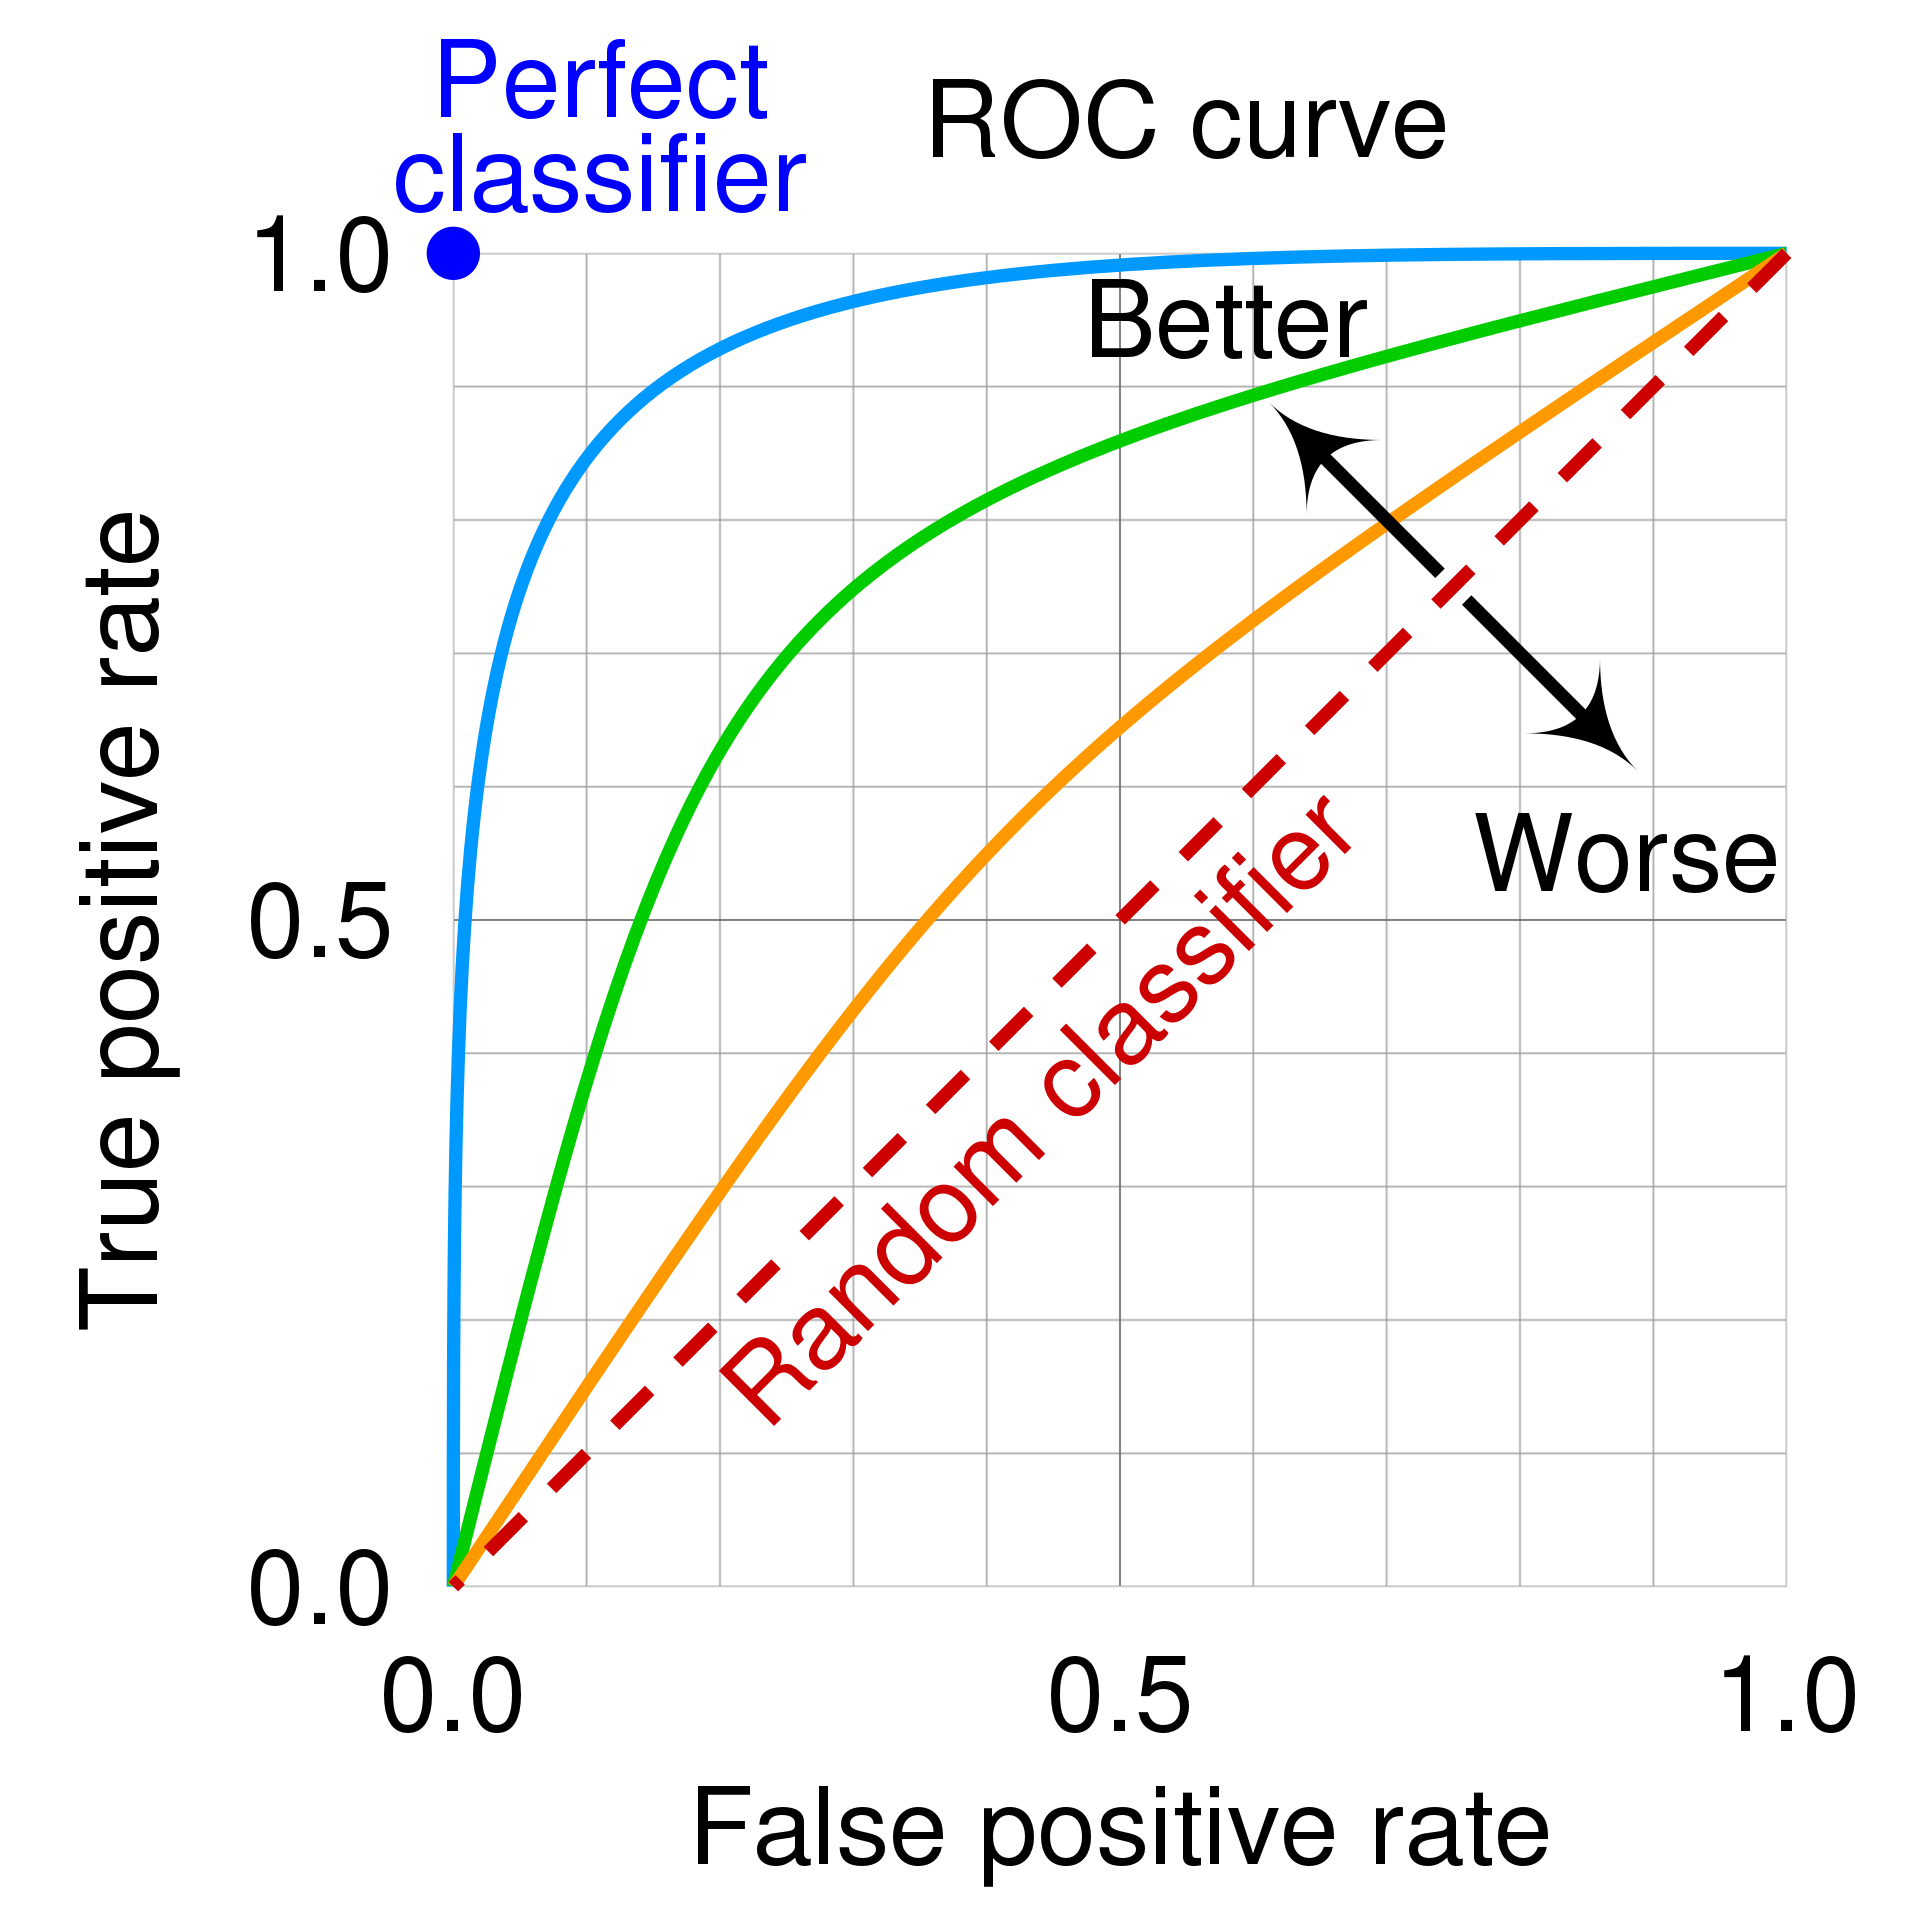
\includegraphics[scale=0.1]{notebooks/Basic/img/roc_curve_diagram.png}
    \caption{ROC Curve Diagram}
    \end{figure}

    El área por debajo de la curva ROC es lo que se conoce como AUC. Una mayor área indica un mejor rendimiento del modelo. 

    Una interpretación de esta medida, se puede entender cómo "La probabilidad de escoger el ejemplo con el label positivo dado que se presenta uno con label positivo y otro con label negativo", o bien, hablar del buen ordenamiento de los ejemplos positivos y los ejemplos negativos. 
    
    \item \textbf{Gini Index: } El índice de Gini se construye de manera similar al AUC, la conversión es directa según 
    $$ 
    \text{Gini} = 2 \cdot \text{AUC} - 1 
    $$
    \begin{figure}[H]
    \center
    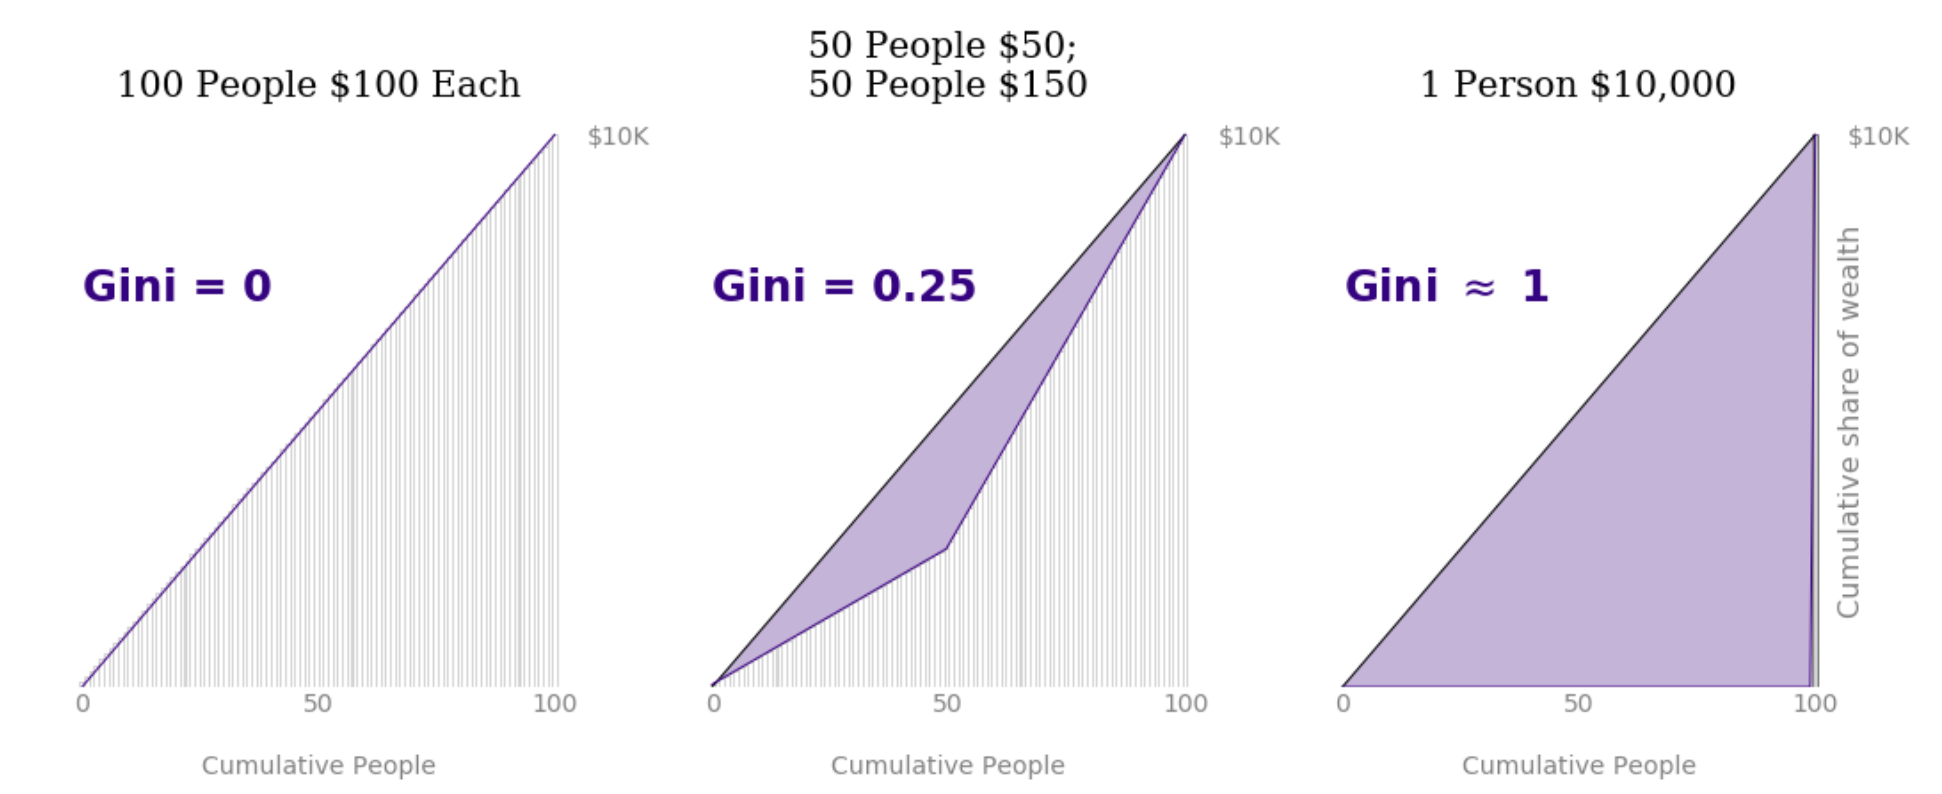
\includegraphics[scale=0.3]{notebooks/Basic/img/gini_diagram.png}
    \caption{Gini Diagram}
    \end{figure}
    
\end{enumerate}

\subsection{Regression Metrics}

Para problemas de regresión, es posible utilizar las siguientes métricas 
\begin{enumerate}
    \item \textbf{MSE}: El error cuadrático medio definido como 
    $$ 
    \text{MSE} = \sqrt{\frac{1}{N}\sum_{i=1}^N(y_i - \hat{y}_i)^2}
    $$
    \item \textbf{MAE}: El error absoluto medio definido como 
    $$ 
    \text{MAE} = \frac{1}{N}\sum_{i=1}^N|y_i - \hat{y}_i|
    $$
    \item \textbf{R Squared}: El coeficiente de determinación $R^2$ es ampliamente utilizado para medir el poder predictivo de una regresión lineal. Es un valor que oscila entre 0 y 1 y está definido como 
    $$ 
    R^2 = 1 - \frac{SS_{\text{res}}}{SS_{\text{tot}}}
    $$
    Donde $SS_{\text{res}}$ es la suma de los cuadrados de las diferencias entre el valor real y la predicción. $SS_{\text{tot}}$ es la suma de los cuadrados de las diferencias entre el valor real y el valor medio de la variable (similar al cálculo de varianza). 

    \begin{figure}[H]
    \center
    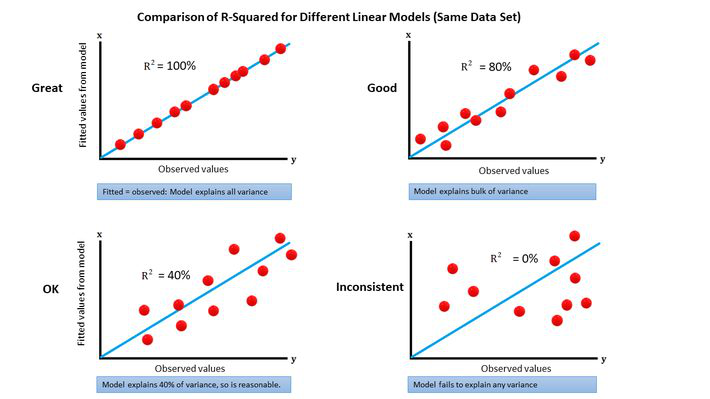
\includegraphics[scale=0.1]{notebooks/Basic/img/r_squared_diagram.png}
    \caption{R Squared Diagram}
    \end{figure}

    Existe una variación \textbf{Adjusted R Squared} que toma en consideración además la cantidad $M$ de features en el modelo. 

    $$
    R^2_{\text{Adjusted}} = 1 - \frac{(1-R^2)(N-1)}{N-M-1}
    $$

    La idea es controlar el overfitting al agregar más variables al modelo mejorando el $R^2$ pero no así el $R^2_{\text{Adjusted}}$.
    
\end{enumerate}

\section{Bias vs Variance}

El dilema de \textit{Bias vs Variance} describe la relación entre la complejidad del modelo, la precisión de las predicciones y cómo éste se comporta al predecir datos nunca antes vistos. El error estimado de una predicción viene dado en términos generales por 
$$
\text{Expected Error} = (\text{Bias})^2 + \text{Variance} + \text{Irreductible Error}
$$
Así, un modelo que crece en complejidad reducirá su bias pero aumentará su varianza (extremo: overfitting) y a la vez, reducir la complejidad permitirá generalizar mejor reduciendo la varianza pero aumentando el bias (extremo: underfitting). 

\begin{figure}[H]
    \center
    \includegraphics[scale=0.27]{notebooks/Basic/img/bias_vs_variance.png}
    \caption{Bias vs Variance Diagram}
\end{figure}

\newpage

\chapter{Machine Learning}

\section{Definition}

Consideremos un conjunto de datos $X = (x_1, \dots , x_N)$ donde para cada $i \in {1, \dots, N}$, $x_i = [x_{i}^1 , \dots, x_{i}^M]$ es decir, un conjunto de $N$ datos con $M$ features cada uno. Consideremos además $Y = (y_1, \dots , y_N)$ las etiquetas o labels cada cada dato. En problemas de clasificación binario, $y_i \in \{ 0, 1\}$ y en problemas de clasificación multiclase, $y_i \in \{1, \dots L\}$. Para problemas de regresión, $Y = (y_1, \dots , y_N)$ con cada $y_i \in \mathbb{R}$.

\section{Linear Regression}

Un modelo de regresión lineal es un modelo de aprendizaje \textbf{supervisado} utilizado para problemas de \textbf{regresión} y \textbf{clasificación}. Se construye a través de la búsqueda de parámetros $\beta_0, \dots, \beta_M$ que multiplican el input para obtener la predicción. En problemas de regresión, 
$$\hat{y} = f(\beta) = \beta_0 + \sum_{j=1}^M \beta_j x^j$$
y en problemas de clasificación a través de una función sigmoide 
$$\hat{y} = f(\beta) = \frac{1}{1+e^{- (\beta_0 + \sum_{j=0}^M \beta_j x^j)}}$$.

\begin{figure}[H]
    \center
    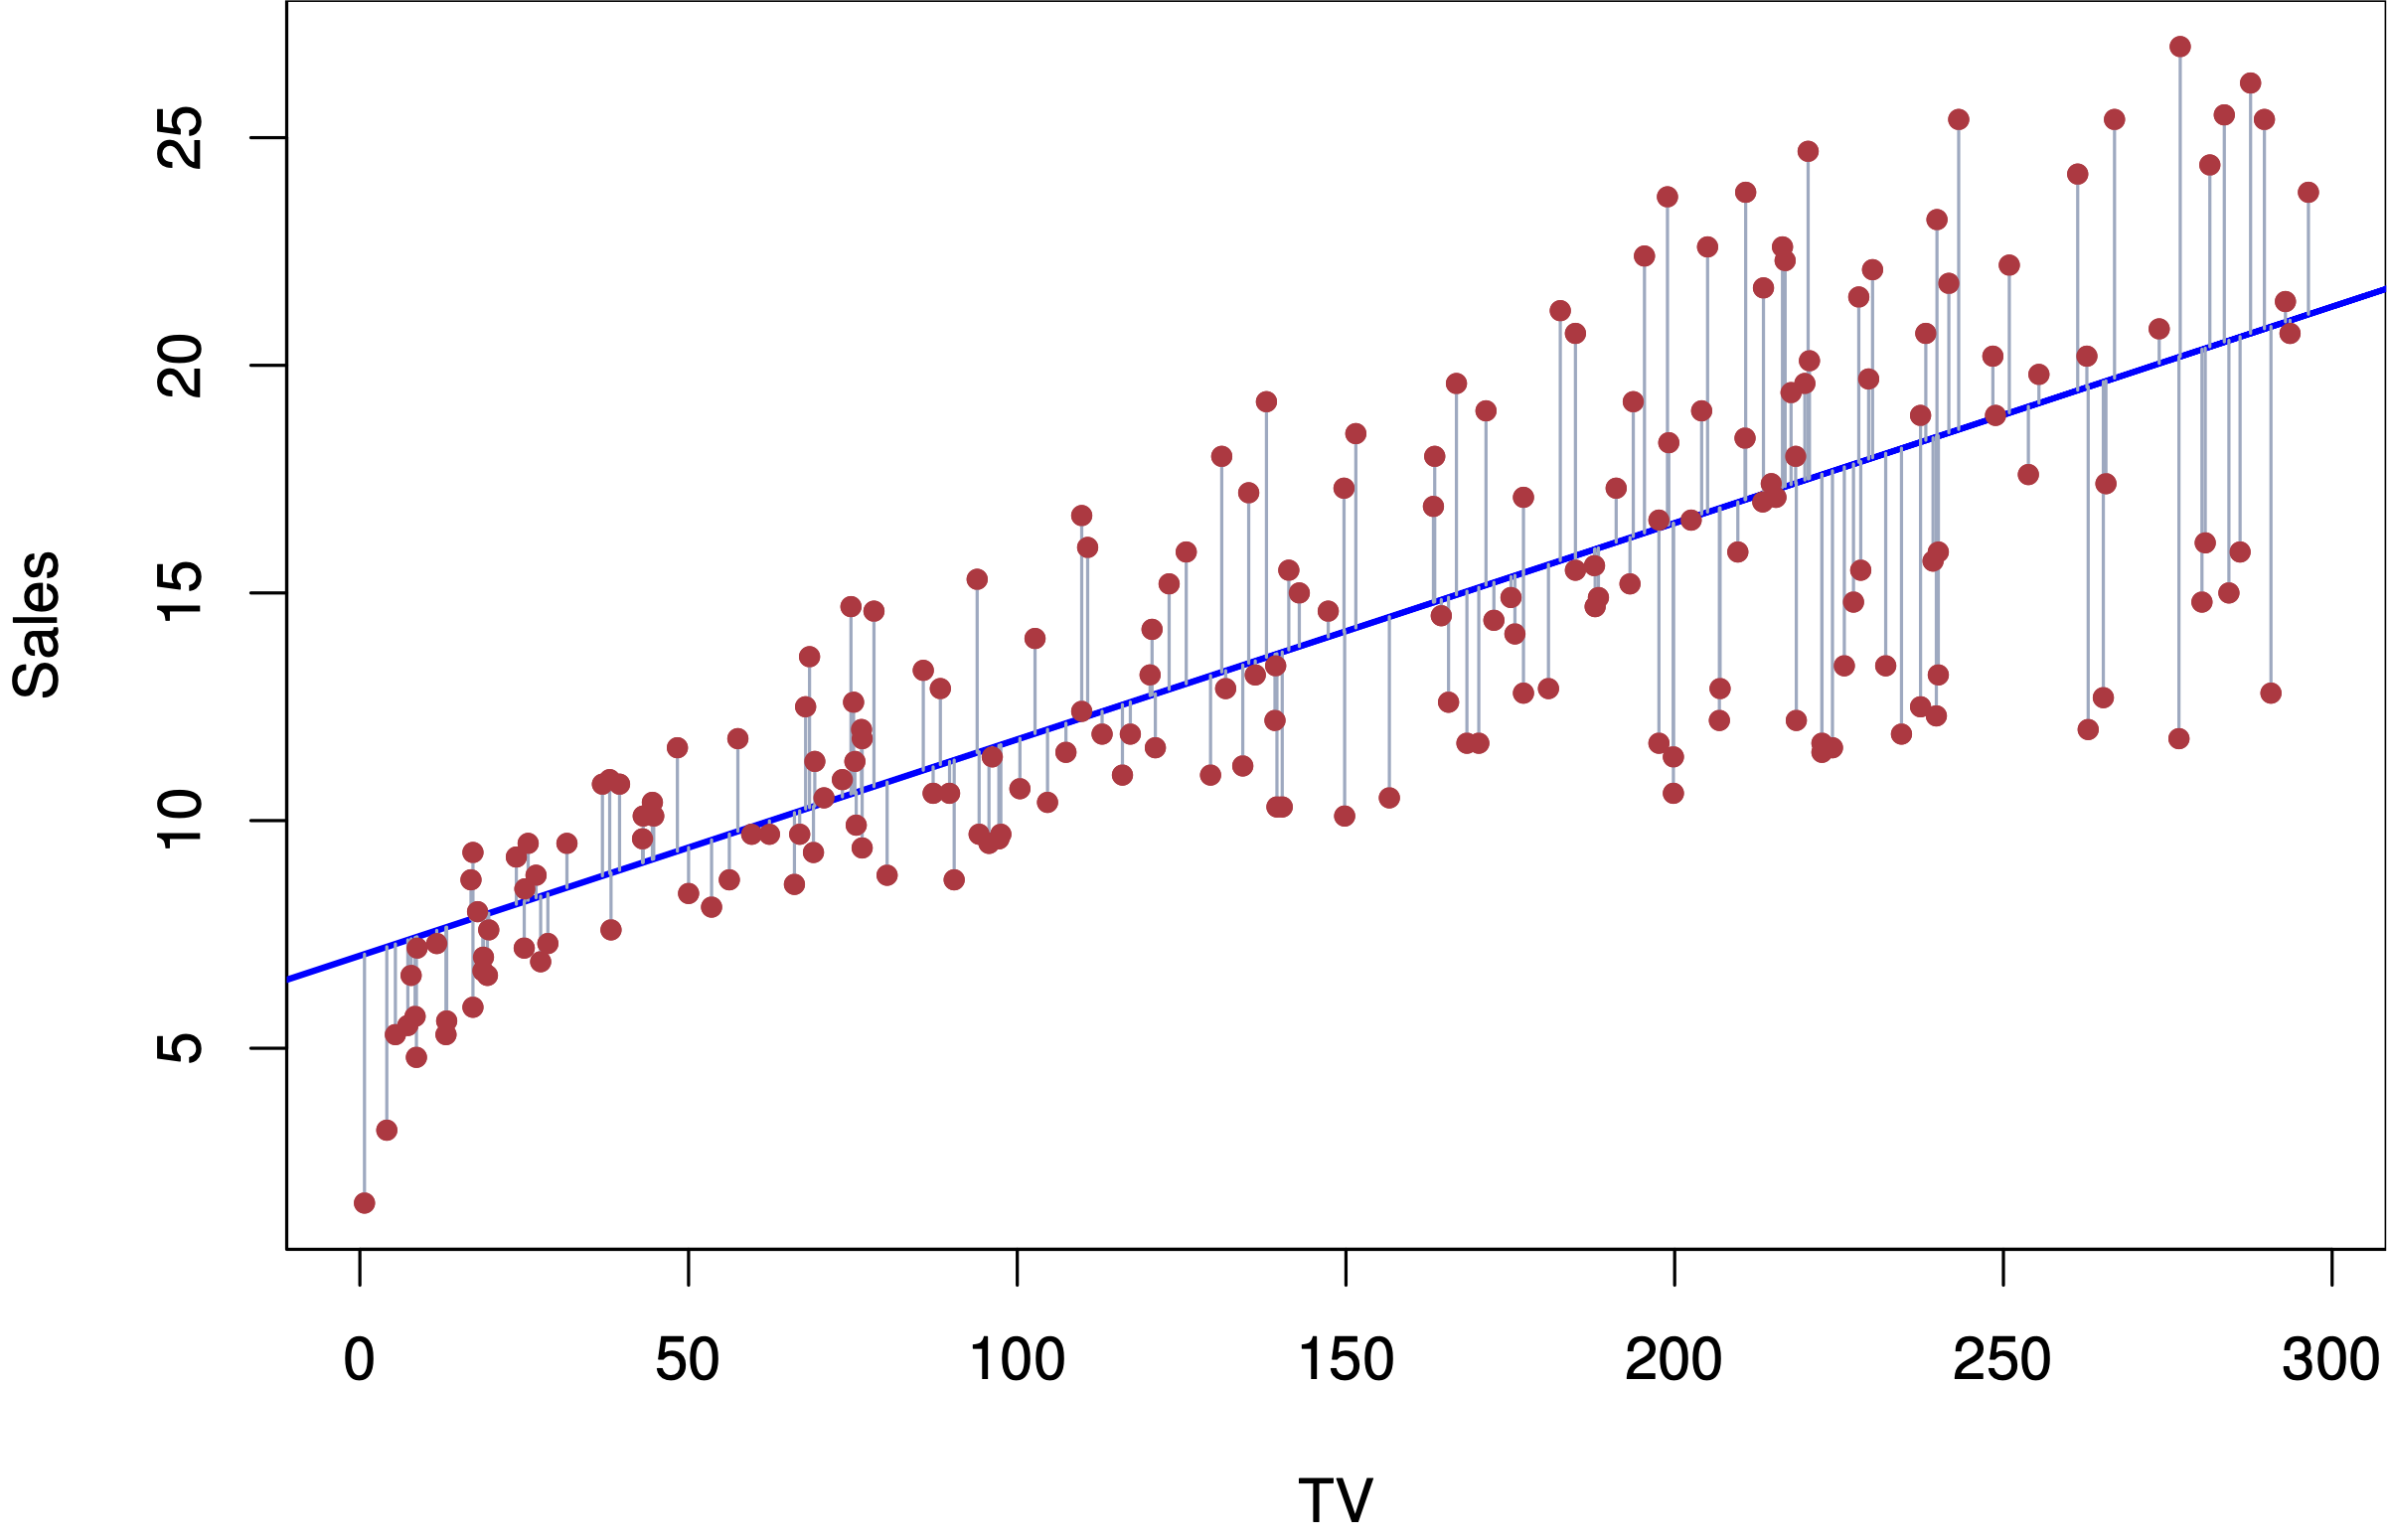
\includegraphics[scale=0.5]{notebooks/ML/img/linear_regression_diagram.png}
    \caption{Linear Regression Diagram}
\end{figure}

El problema a optimizar (mínimos errores cuadrados) queda entonces definido por 
$$\min_{\beta} \quad \frac{1}{N}\sum_{i=1}^N(y_i - f(\beta))^2$$
Cuya solución es cerrada en el caso de estimar una regresión y estimada a través del descenso de gradiente en el caso de una clasificación. 

\subsection{Regularization}

Para prevenir el overfitting y que la importancia de los parámetros quede mejor distribuida, es posible agregar a la función un término regularizador de la siguiente forma

\begin{equation*}
\begin{aligned}
\min_{\beta} \quad \frac{1}{N}\sum_{i=1}^N(y_i - f(\beta))^2 \\
\textrm{s.t.} \quad ||\beta||^{p}_{p} \leq t
\end{aligned}
\end{equation*}

De manera equivalente, por el método de \textit{Lagrange}, sin optimizar el valor de $\lambda$ y eliminando constantes que no dependen de $\beta$
$$\min_{\beta} \quad \frac{1}{N}\sum_{i=1}^N(y_i - f(\beta))^2 + \lambda ||\beta||^{p}_{p}$$
Cuando $p=1$ se le conoce como regresión \textbf{Lasso} y cuando $p=2$ una regresión \textbf{Ridge}. La combinación de ambas restricciones es conocida como \textbf{Elastic Net}. 

\begin{figure}[H]
    \center
    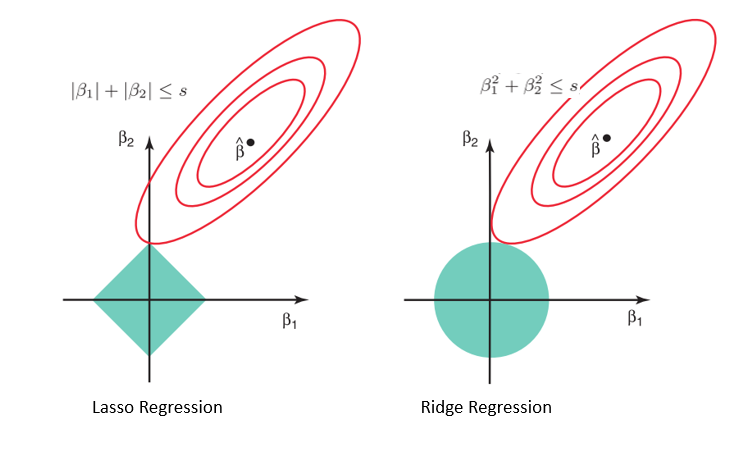
\includegraphics[scale=0.4]{notebooks/ML/img/lasso_and_ridge_diagram.png}
    \caption{Lasso and Ridge Diagram}
\end{figure}

Notar que la restricción para el caso \textit{Lasso} hace más probable que las curvas de nivel intersecten la restricción en una esquina (en mayor dimensión es incluso más probable) por lo que los parámetros que no son importantes para el modelo, serán llevados a 0. En el caso de la restricción \textit{Ridge}, la forma permite que los valores queden acotados pero ninguno será llevado a 0.

\begin{figure}[H]
    \center
    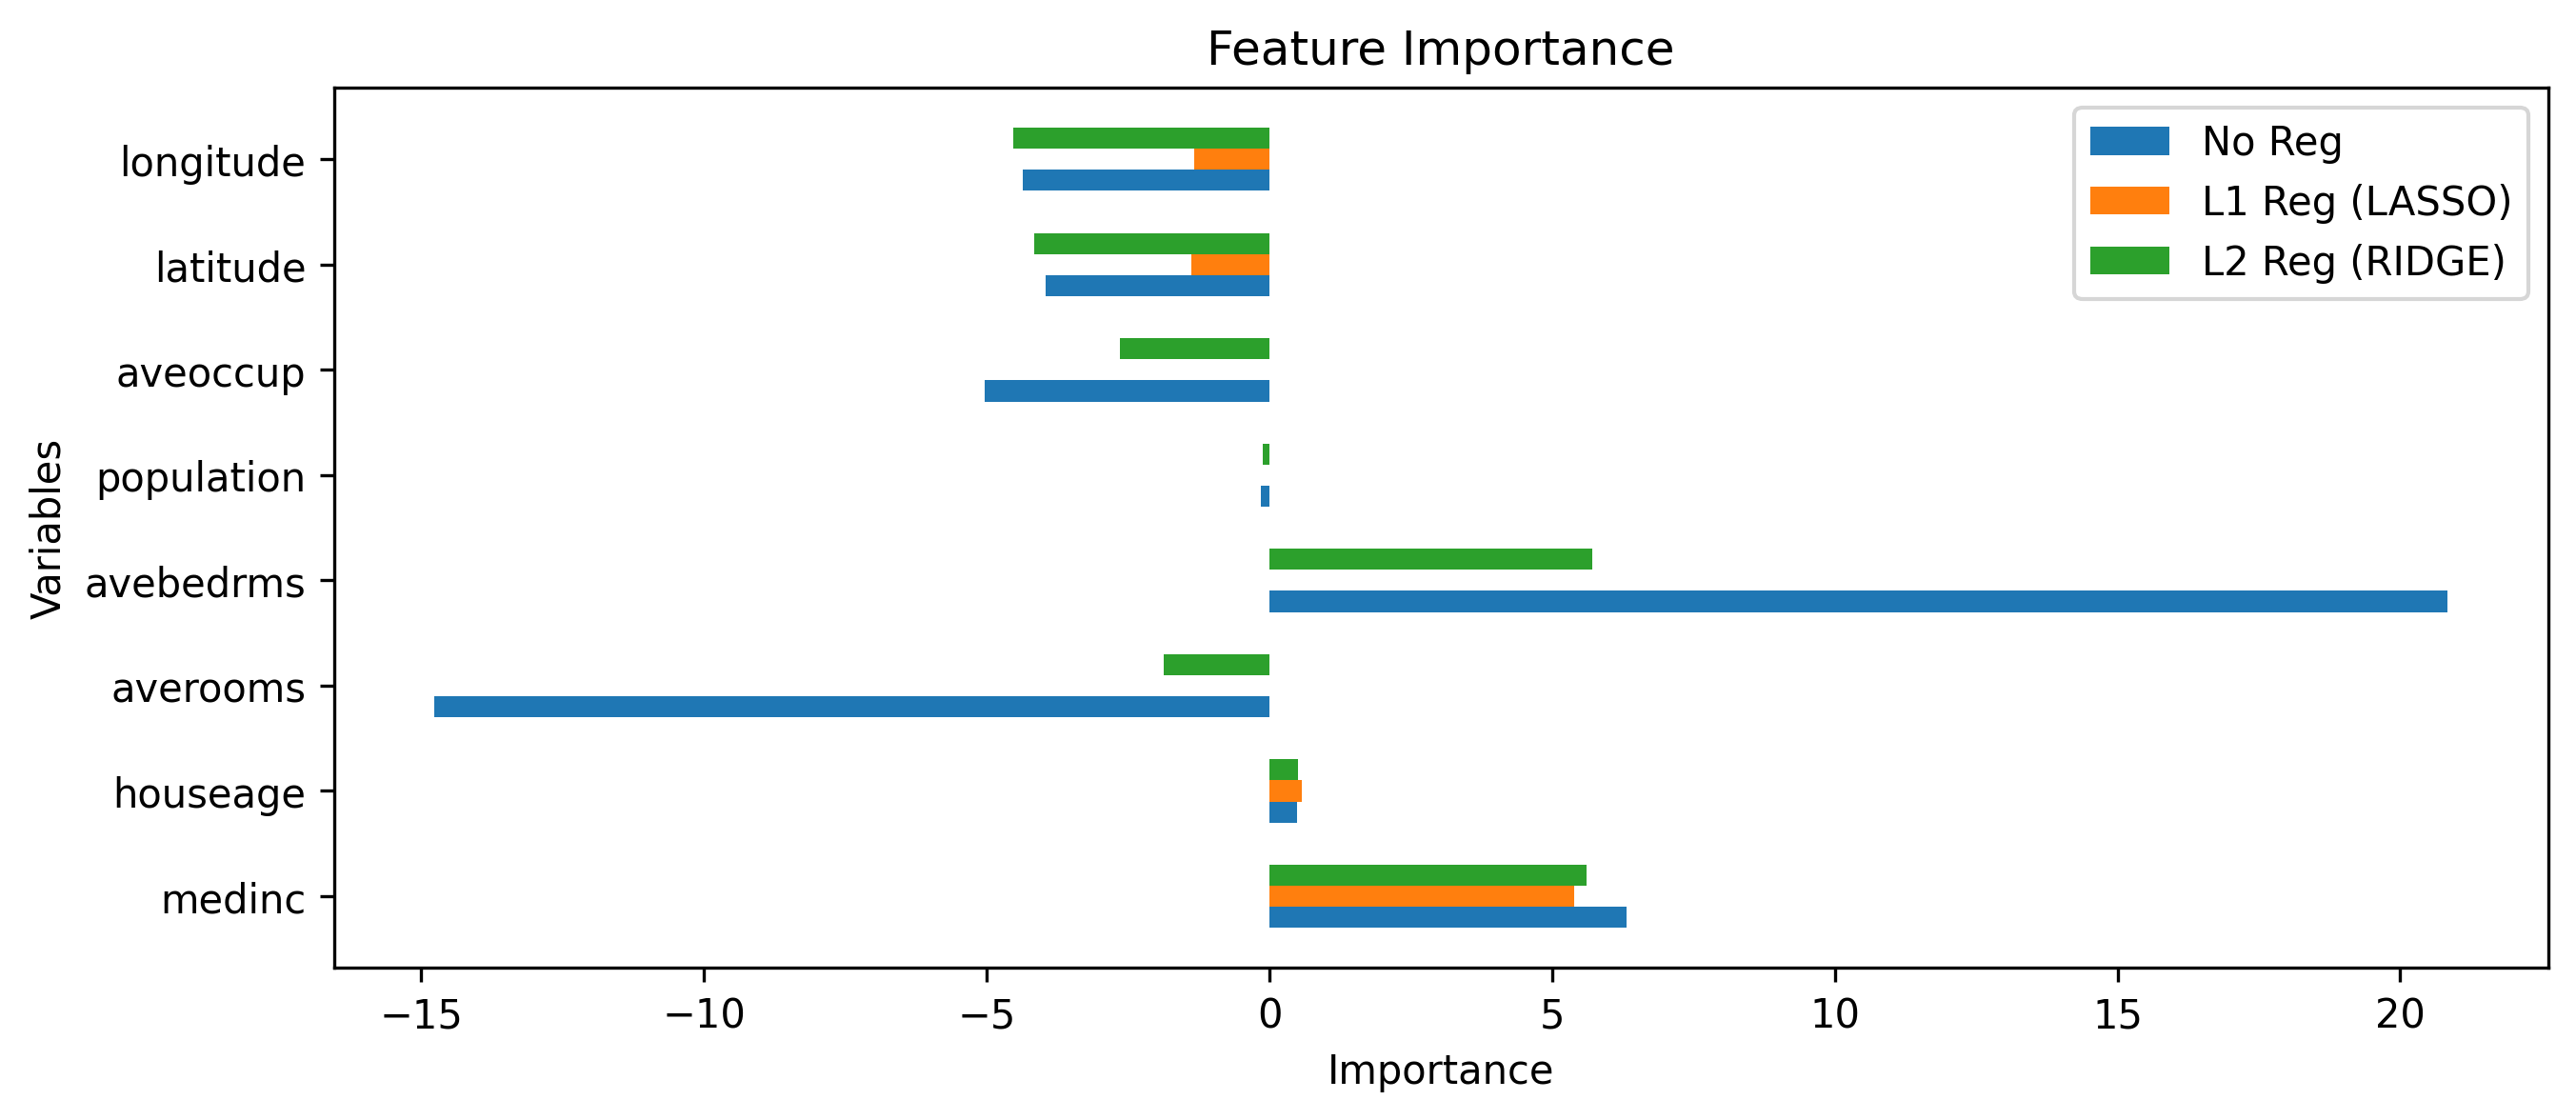
\includegraphics[scale=0.5]{notebooks/ML/img/regularization_feature_importance.png}
    \caption{Regularization Feature Importance}
\end{figure}


\section{Decision Trees}

Un árbol de decisión es un modelo de aprendizaje \textbf{supervisado} utilizado para problemas de \textbf{regresión} y \textbf{clasificación}. El objetivo es aprender simples reglas de decisión a partir de las features. 

\begin{figure}[H]
    \center
    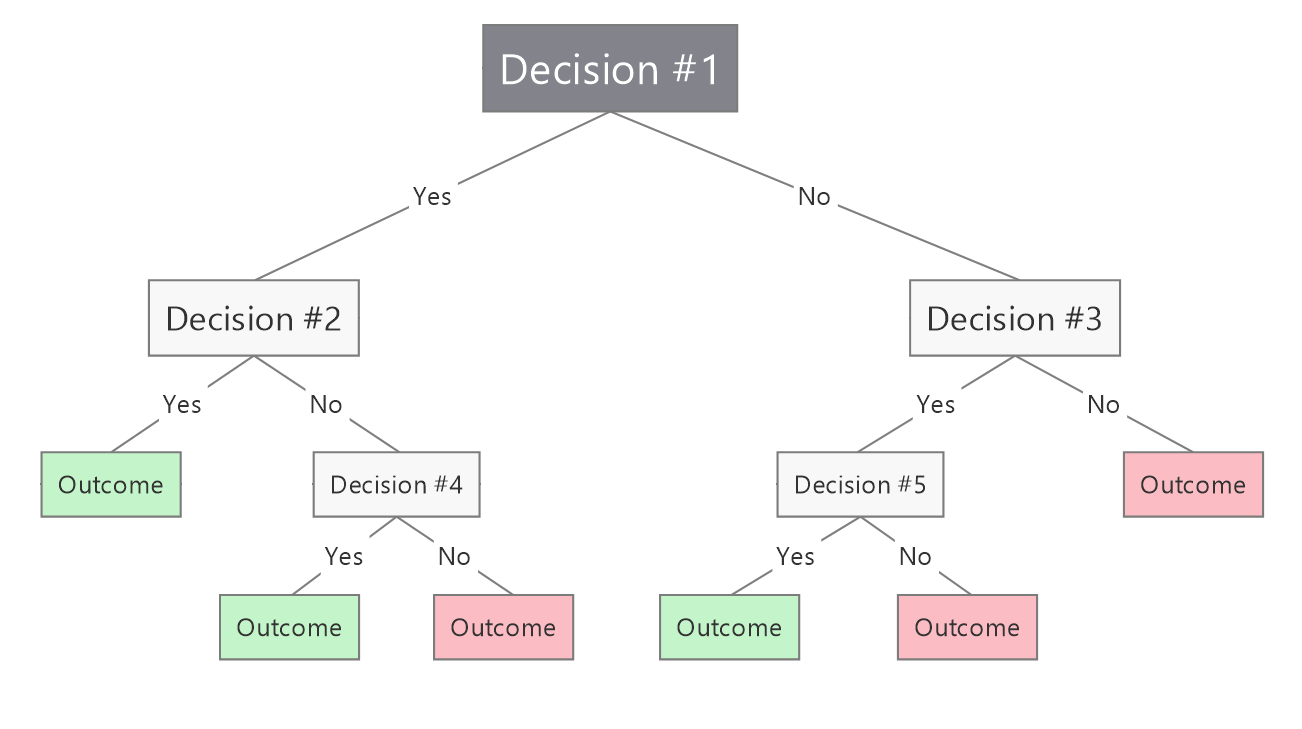
\includegraphics[scale=0.25]{notebooks/ML/img/decision_tree_diagram.png}
    \caption{Decision Tree Diagram}
\end{figure}

En el caso de un problema de clasificación, la variable a escoger y el corte correspondiente se puede elegir como aquel que minimice el desorden de los elementos. Definimos primero la \textbf{entropía} según 
$$H(p) = - \sum_{j=1}^{L}p_j\log_{2}p_j$$

donde $p_j$ es la frecuencia relativa del label $j$ en un grupo. Notar que la entropía es mínima cuando el grupo solo tiene elementos de la clase 0 o de la clase 1 ($p_j = 1$) y máxima cuando hay la misma cantidad de elementos de cada clase ($p_j = \frac{1}{2}$). 

\begin{figure}[H]
    \center
    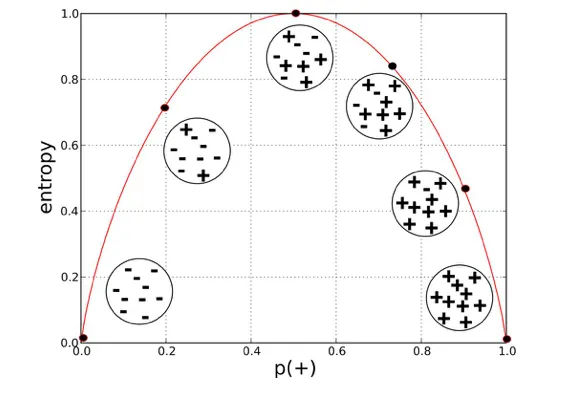
\includegraphics[scale=0.3]{notebooks/ML/img/entropy_diagram.png}
    \caption{Entropy Diagram}
\end{figure}

Con la entropía ya definida, definamos la \textbf{Information Gain} como 
$$IG(S,D) = H(S) - \sum_{V \in D}\frac{|V|}{|D|}H(V)$$

Donde el primer término es la entropía antes del split y el segundo término es la suma de las entropías después del split. Podemos iterar hasta que la \textit{Information Gain} no tenga modificaciones (es decir, llegar a los nodos puros) pero esto podría traer problemas de overfitting, en general esto se regula con la profundidad del árbol y escogiendo en cada iteración, la división que maximiza el IG. 

\begin{figure}[H]
\begin{subfigure}{.5\textwidth}
    \center
    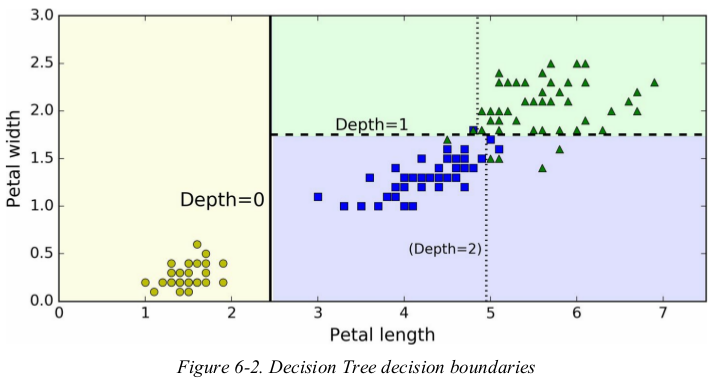
\includegraphics[scale=0.3]{notebooks/ML/img/decision_tree_data.png}
    \caption{Decision Tree Boundaries}
\end{subfigure}%
\begin{subfigure}{.5\textwidth}
    \center
    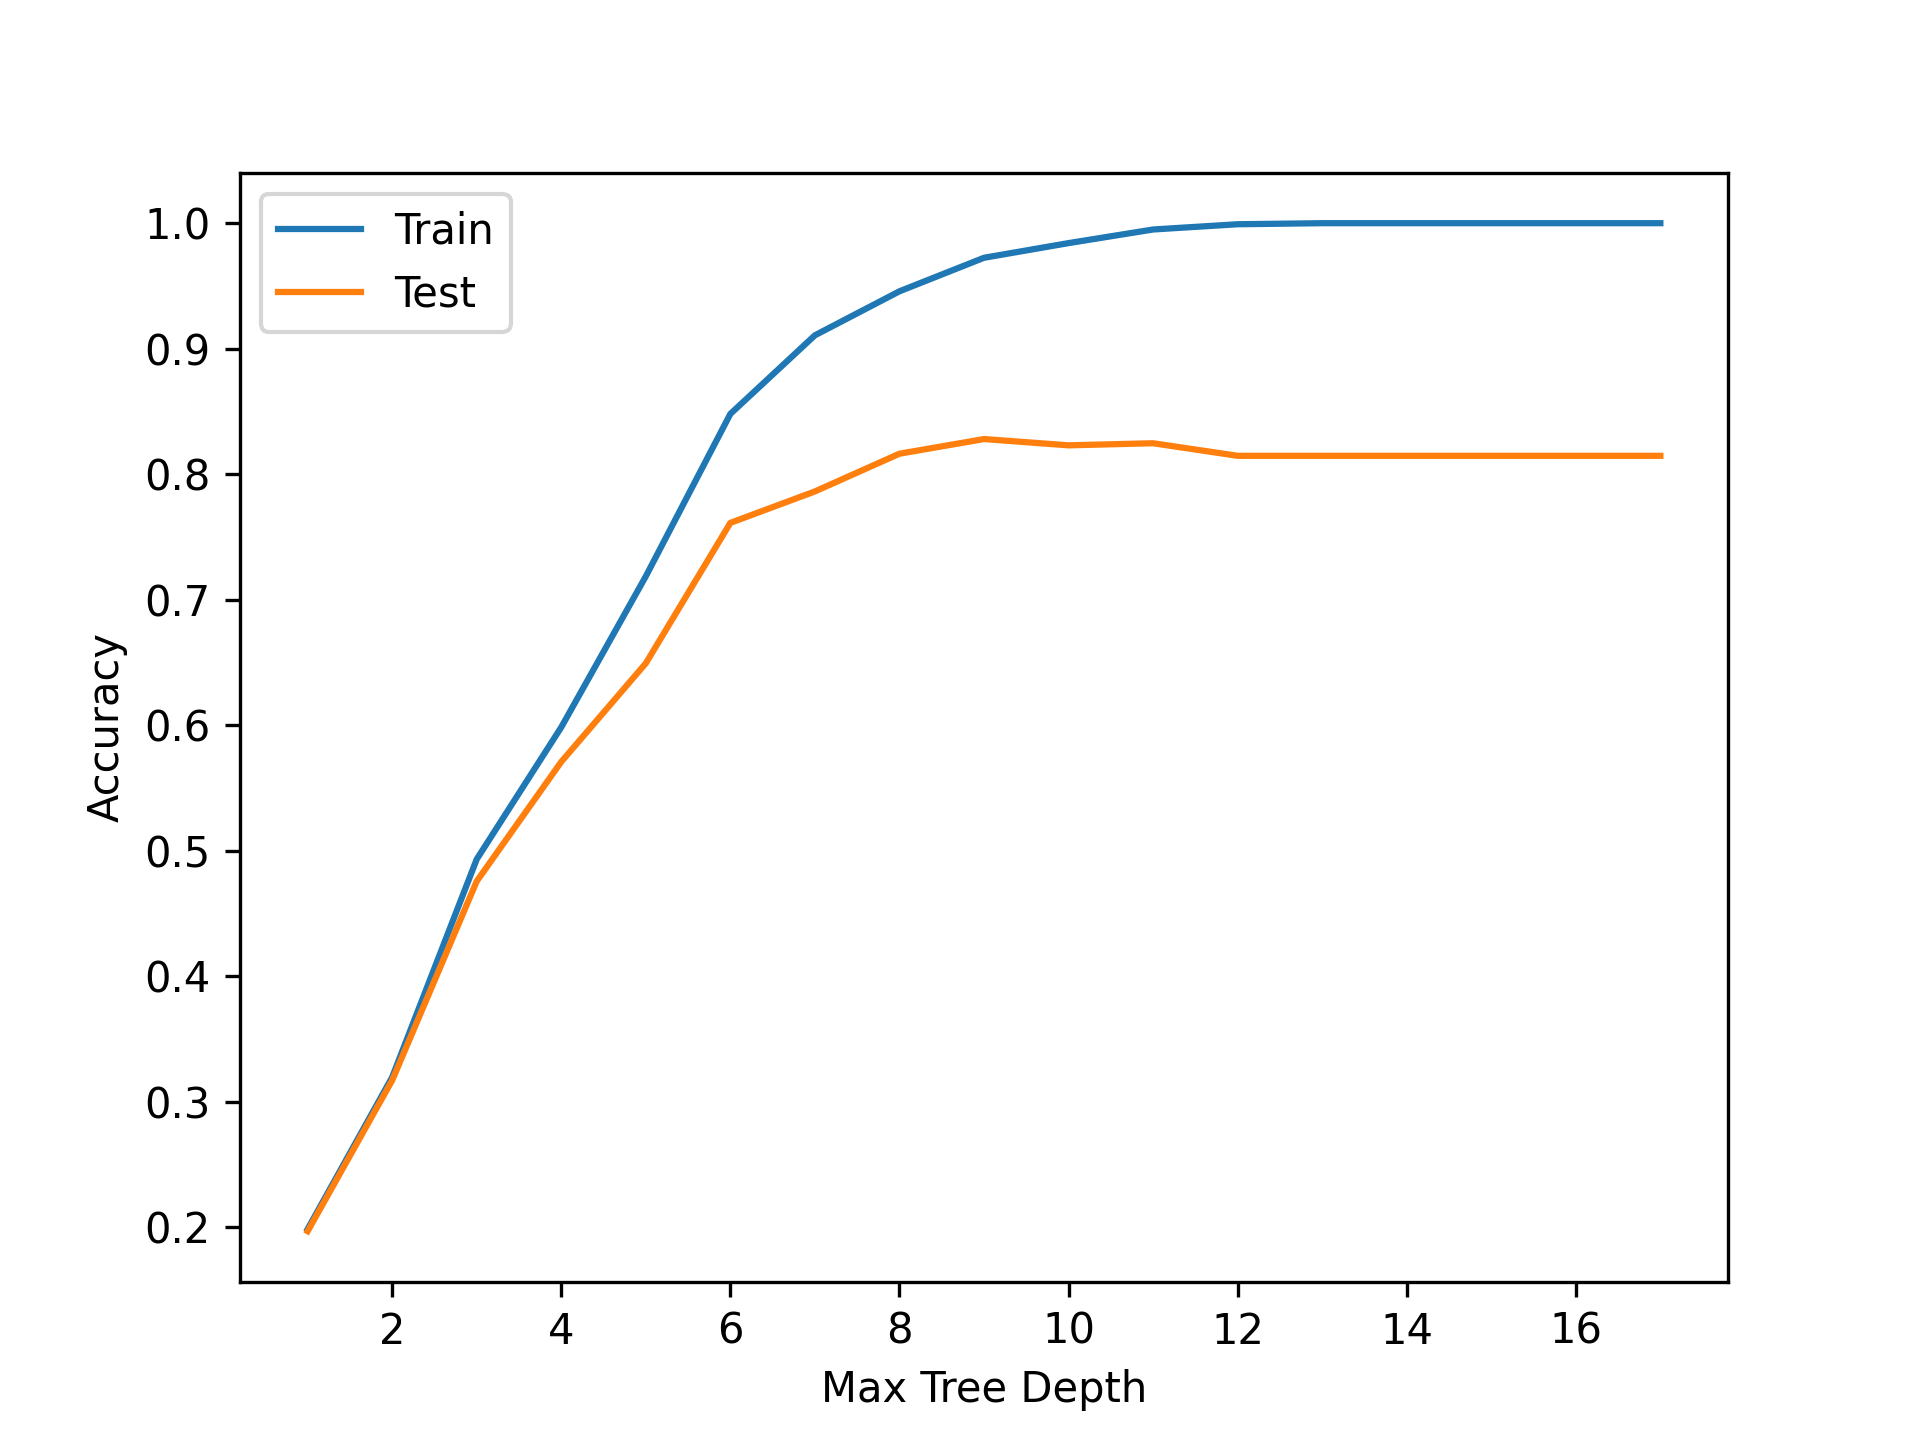
\includegraphics[scale=0.4]{notebooks/ML/img/max_depth_decision_tree.png}
    \caption{Max Depth and Accuracy}
\end{subfigure}
\caption{Decision Tree Implementation}
\label{fig:fig}
\end{figure}

En vez de la entropía, es posible usar otro indicador como el \textbf{Gini Index} definido como: 
$$G(p) = 1 - \sum_{j=1}^L p_j^2$$

\section{Random Forest}

\subsection{Ensemble Methods}

Los \textbf{métodos de ensamblaje} son aquellos en los que se combinan múltiples estimadores entrenados sobre los datos para generar una predicción más robusta (menor varianza) y generalizada. La predicción final se puede realizar por \textit{Majority Voting}, \textit{Simple Average} o \textit{Weighted Average}.

Existen 3 estrategias principales en los métodos de ensamblaje: 
\begin{enumerate}
    \item \textbf{Bagging}: Corresponde a una abreviación de \textit{Bootstrap Aggregating}, esta estrategia entrena cada estimador base con una \textbf{muestra con reemplazo} de ejemplos del conjunto de entrenamiento. (\textbf{Reduce la varianza})
    \item \textbf{Boosting}: Esta estrategia se basa en entrenar secuencialmente estimadores base débiles que \textbf{aprenden de los errores del anterior} para crear un estimador robusto. (\textbf{Reduce el bias})
    \item \textbf{Stacking}: Este método combina las predicciones de múltiples estimadores fuertes en una sola. 
\end{enumerate}

\begin{figure}[H]
    \center
    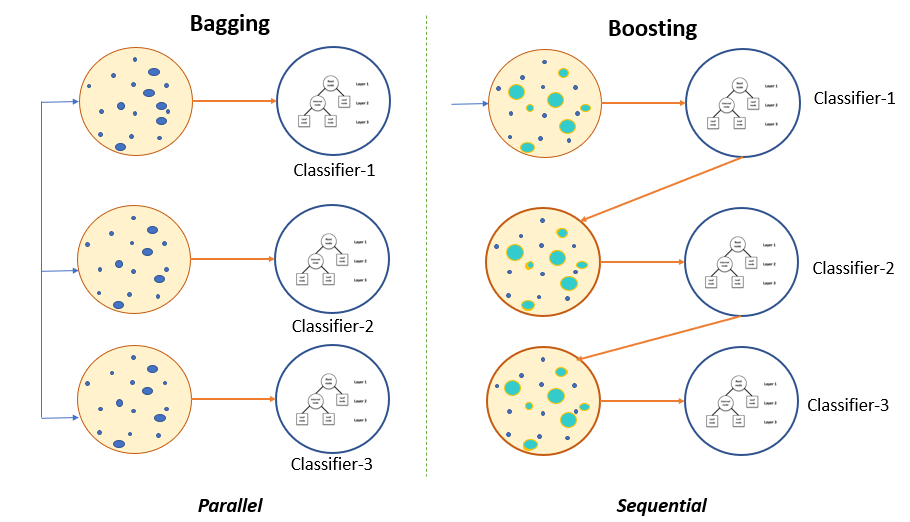
\includegraphics[scale=0.25]{notebooks/ML/img/bagging_and_boosting_diagram.png}
    \caption{Bagging and Boosting Diagram}
\end{figure}


El algoritmo de \textit{Random Forest} es un método \textbf{supervisado de ensamblaje} basado en \textit{Decision Trees}. Este, utiliza la estrategia de \textbf{bagging} para entrenar cada árbol de decisión sobre muestras con reemplazo del conjunto de entrenamiento y además, cada árbol es entrenado sobre un \textbf{subconjunto aleatorio de features} para asegurar que no haya similitud entre ellos. Ambas estrategias permiten mejorar la precisión del modelo y controlar el overfitting.

\begin{figure}[H]
    \center
    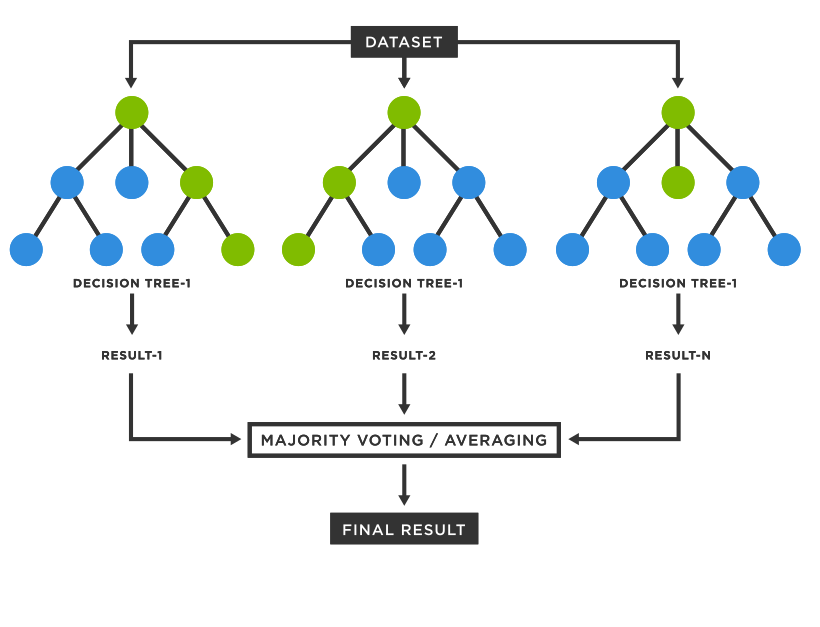
\includegraphics[scale=0.25]{notebooks/ML/img/random_forest_diagram.png}
    \caption{Random Forest Diagram}
\end{figure}

Para estimar la \textbf{feature importance} en modelos basados en árboles, se pueden mirar 3 posibles aspectos: 
\begin{enumerate}
    \item Suma de las \textit{information gain} con una variable determinada (o cuánto reduce la entropía, es equivalente). 
    \item Cantidad de nodos resultantes de la división con esa variable. 
    \item Profundidad promedio de un árbol en que su primera división es con esa variable. 
\end{enumerate}

Para extender esto a \textit{Random Forest}, se toma un promedio entre los distintos árboles de decisión que lo conforman. 

\section{Gradient Boosting Algorithm}

Los modelos de \textit{Gradient Boosting} son algoritmos basados en árboles que pueden ser utilizados para problemas de \textbf{clasificación y regresión}. 

\begin{figure}[H]
    \center
    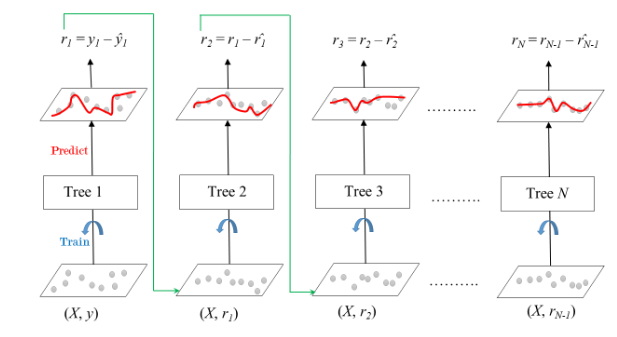
\includegraphics[scale=0.5]{notebooks/ML/img/gbc_diagram.png}
    \caption{Gradient Boosting Diagram}
\end{figure}

El entrenamiento consta en el aprendizaje secuencial de árboles de baja complejidad (\textit{weak learners}) que aprenden de los errores del anterior, vale decir, que aprenden en el conjunto de los \textbf{residuos} del modelo anterior. Sea $L(y , F(x))$ el error de la predicción del modelo $F(x)$ y el valor real $y$. 

El modelo $F(x)$ es el resultado de una combinación lineal de \textit{weak learners} tal que 
$$ 
F(x) = \sum_{k=1}^T \gamma_k h_k(x)
$$
Donde T es la cantidad de árboles (\textit{n estimators}), $h_k$ los  \textit{weak learners} y $\gamma_k$ su peso. Iniciando en un modelo inicial $F_0(x)$ entrenado sobre los datos, cada iteración se encarga de construir $F_{k}(x)$ según 
$$ 
F_{k} = F_{k-1} + \gamma_{k}h_{k}
$$
Para encontrar los valores $\gamma_{k} , h_{k}$ se siguen los siguientes pasos: 
\begin{enumerate}
    \item Calcular los residuos $i$ en la iteración $k$ como $r_{i,k} = - \left [ \frac{\partial L(y_i, F(x_i))}{\partial F(x_i)} \right ]_{F(x) = F_{k-1}(x)}$. En el caso de $L$ una función de error MSE, $r_{i,k} = 2(y_i - F_{k-1}(x_i)) \propto y_i - F_{k-1}(x_i)$
    \item Entrenar un \textit{weak learner} sobre $(X, r)$.
    \item Encontrar el valor de $\gamma_k$ como aquel que resuelve 
    $$ 
    \gamma_k = \argmin_{\gamma}\sum_{i=1}^N L(y_i , F_{k-1} + \gamma h_{k}(x_i))
    $$
    \item Hacer update al modelo según $F_{k} = F_{k-1} + \gamma_{k}h_{k}$
\end{enumerate}

La importancia de las variables es medida de manera similar a un \textit{Random Forest}, a través de la suma ponderada de las \textit{Information Gain} (o bien de la disminución de la entropía) que cada una de las features provoca en los distintos árboles. 

Existen otras formas de calcular la importancia de las variables, lo cual se discute en la sección \ref{subsec:shap_values}.

\section{Naive Bayes}

Este modelo de aprendizaje \textbf{supervisado} puede ser utilizado para problemas de clasificación. Este algoritmo es una aplicación del teorema de \textit{Bayes} en el que se asume (\textit{Naive}) la independencia condicional entre los pares de features $x^j$ dado el valor del label $y$

\begin{figure}[H]
    \center
    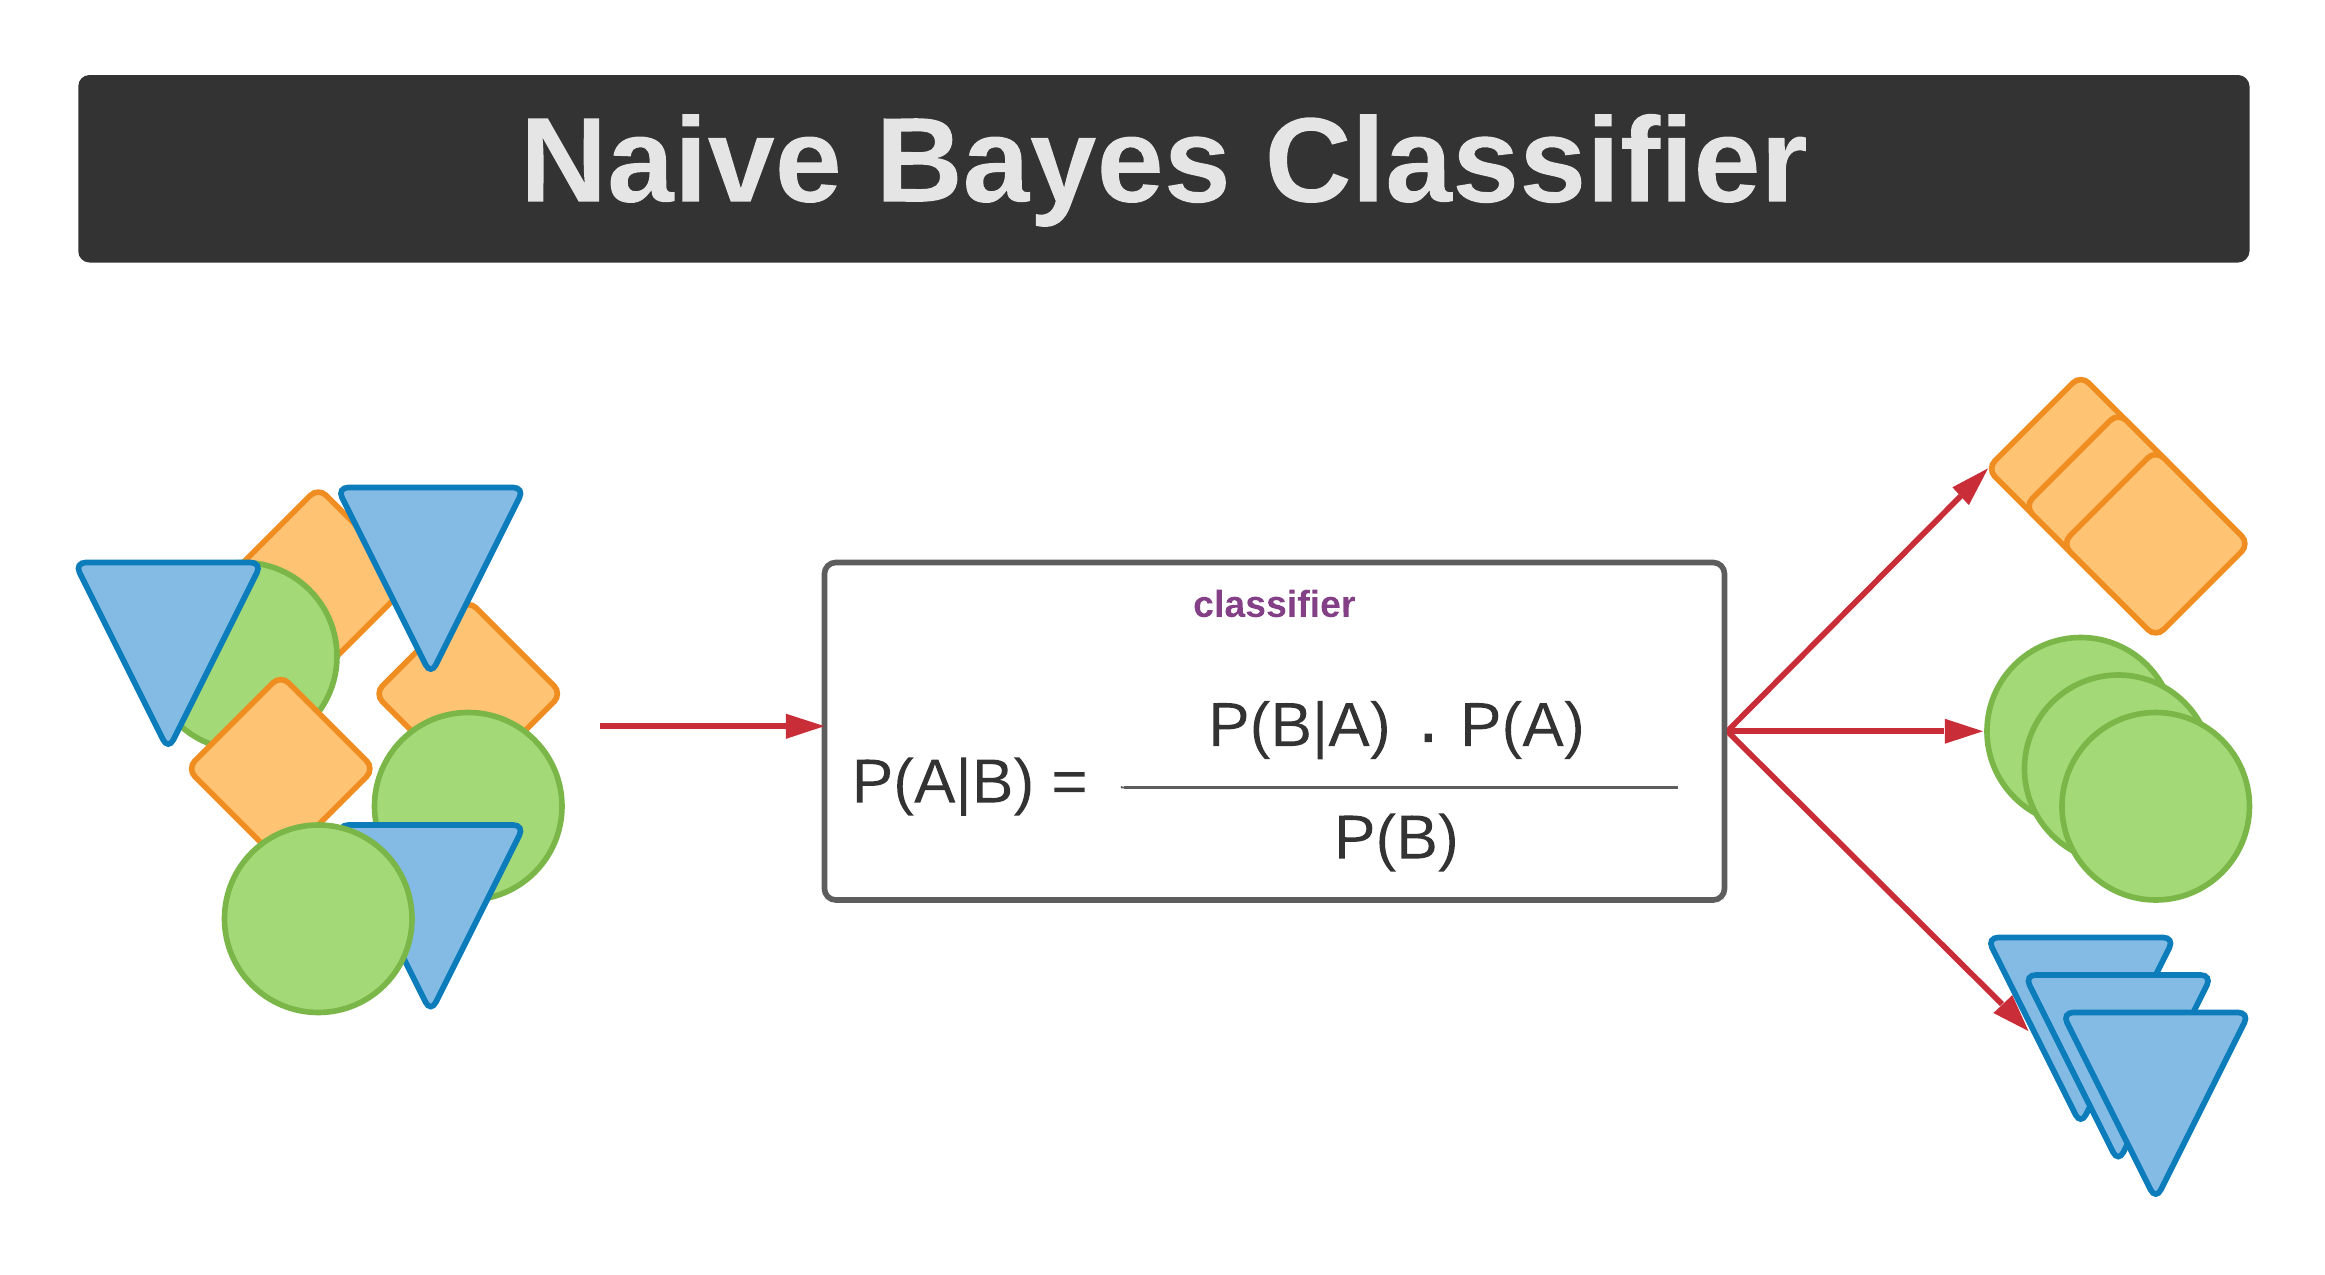
\includegraphics[scale=0.4]{notebooks/ML/img/naive_bayes_diagram.png}
    \caption{Naive Bayes Diagram}
\end{figure}

La formulación es la siguiente: 
$$
P(y | x^1 , \dots , x^M) = \frac{P(y)P(x^1 , \dots , x^M| y)}{P(x^1 , \dots , x^M)} = \frac{P(y)\prod_{j=1}^M P(x^j | y)}{P(x^1 , \dots , x^M)} \propto P(y)\prod_{j=1}^M  P(x^j | y)
$$
y la predicción se realiza según 
$$
\hat{y} = \text{argmax}_{y} P(y)\prod_{j=1}^M  P(x^j | y)
$$

\subsection{Gaussian Naive Bayes}

Aquí consideramos que $x^{j} | y \sim \mathcal{N}(\mu_j , \sigma_j^2)$ , es decir, cada feature sigue una distribución normal según:
$$
P(x^j | y) = \frac{1}{\sqrt{2\pi\sigma_j^2}}\exp \left(- \frac{(x^j - \mu_j)^2}{2\sigma_j^2} \right )
$$
donde la media y varianza $\mu_j$ y $\sigma_j$ respectivamente, son calculados a través de la máxima verosimilitud, es decir, si $x_{i} = (x^{1}_i, x^{2}_i, \dots x^{M}_i)$ con $i \in \{1, \dots, N\}$ los datos, entonces
$ \mu_{j} = \frac{1}{N}\sum_{i=1}^{N}x_{i}^{j}$ y $ \sigma_{j} = \frac{1}{N-1}\sum_{i=1}^{N}(x_{i}^{j}-\mu_{j})^2$. Notar que esto se debe calcular utilizando los datos de la clase respectiva $y$. 

La definición anterior funciona bien con tipos de data numéricos. 

\begin{figure}[H]
    \center
    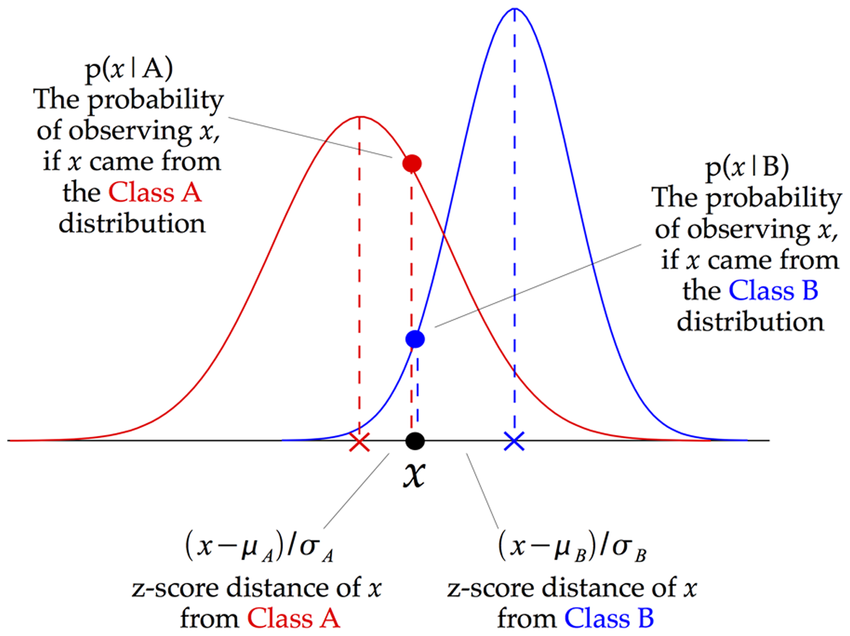
\includegraphics[scale=2]{notebooks/ML/img/gaussian_naive_bayes_diagram.png}
    \caption{Gaussian Naive Bayes Diagram}
\end{figure}

\subsection{Multinomial Naive Bayes}

Aquí consideramos que $x^j | y$ sigue una distribución multinomial donde los parámetros $(p_{j_1}, \dots , p_{j_k})$ de esta distribución son calculados según 
$$
p_{j_k} = \frac{N_{j_k} + \alpha}{N_j + \alpha}  
$$

Donde $N_{j_k}$ es la cantidad de veces que la categoría $k$ de la feature $j$ aparece en los datos con clase $y$ del conjunto de entrenamiento y $N_j = \sum_k N_{j_k}$. El parámetro $\alpha$ es un \textit{Smoothing Prior} para estabilidad numérica. 

La definición anterior funciona bien con tipos de datos categóricos. 

\section{Support Vector Machines}

Las \textit{Support Vector Machines} o SVM, son modelos de aprendizaje \textbf{supervisados} que pueden ser usados para problemas de clasificación y regresión. Se construyen a partir de la búsqueda de un hiper-plano separador y vectores de soporte que maximizan la distancia entre las clases. 

\begin{figure}[H]
    \center
    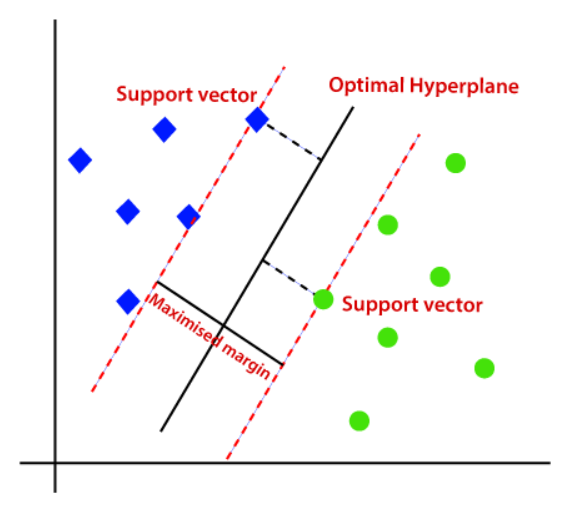
\includegraphics[scale=0.3]{notebooks/ML/img/svm_diagram.png}
    \caption{SVM Diagram}
\end{figure}

Consideremos el caso binario donde $Y \in \{0,1\}^n$ El hiper-plano separador está definido por 
$$ H = \{ x \in \mathbb{R}^n | w^{\top}x + b = 0 \} $$ 
Donde $w$ es el vector perpendicular al hiper-plano y $b$ un offset. 
De esta forma si $w^{\top}x + b > 0$ quiere decir que $x$ pertenece a la clase 1 y $w^{\top}x + b < 0$ que $x$ pertenece a la clase 0, escrito de otra forma 
$$y_i(w^{\top}x+b) \geq 1 \quad \forall i \in \{ 1 , \dots , N \}$$
En el caso de un problema de clasificación linealmente separable, existen infinitos hiper-planos que satisfacen las condiciones anteriores (basta con rotar ligeramente el hiper-plano) por lo que vamos a exigir además las siguientes condiciones sobre vectores de soporte $x_{-}$ y $x_{+}$. 

\begin{equation*}
\begin{split}
w^{\top}x_{+} + b = 1 \\
w^{\top}x_{-} + b = -1
\end{split}
\end{equation*} 

Notar entonces que con esta condición, es posible calcular el ancho $m$ de la separación entre el hiper-plano y el vector de soporte. Recordemos que la distancia $m$ de un vector $x$ a un hiperplano con vector normal $w$ viene dada por 
$$m = \frac{|\langle w, x \rangle|}{||w||}$$
Considerando la definición de los vectores de soporte, se tiene que 
$$2m = \frac{|\langle w, x_{+} \rangle|}{||w||} + \frac{|\langle w, x_{-} \rangle|}{||w||} = \frac{|1-b|}{||w||} + \frac{|-1-b|}{||w||}$$
Además el offset $b \in [0,1]$ por la definición anterior, así 
$$m = \frac{1}{||w||}$$
Finalmente, el problema de optimización quedaría de la siguiente forma 
\begin{equation*}
\begin{aligned}
\max_{\omega , b} \quad \frac{1}{||w||} \\
\textrm{s.t.} \quad y_i(w^{\top}x_i + b ) \geq 1 , \forall i \in \{ 1 , \dots N \}
\end{aligned}
\end{equation*}
Equivalente a 
\begin{equation*}
\begin{aligned}
\min_{\omega , b} \quad \frac{1}{2}||w||^2 \\
\textrm{s.t.} \quad y_i(w^{\top}x_i + b ) \geq 1 , \forall i \in \{ 1 , \dots N \}
\end{aligned}
\end{equation*}
Este problema se resuelve utilizando el \textbf{dual} (\textit{quadratic programming}) y es fundamental para la extensión no-lineal de la SVM (\textit{Kernel Trick}). 

\subsection{Soft Margin}

Los datos son usualmente no linealmente separables, por lo que hay que permitir un error en la clasificación de ciertos puntos (\textit{soft margin}). Este cambio en el problema de optimización se reduce a la siguiente regularización:

\begin{equation*}
\begin{aligned}
\min_{\omega , b} \quad \frac{1}{2}||w||^2 + C \sum_{i=1}^N \xi_i  \\
\textrm{s.t.} \quad y_i(w^{\top}x_i + b ) \geq 1  - \xi_i, \forall i \in \{ 1 , \dots N \} \hspace{0.1cm} ,\hspace{0.1cm} \xi_i \geq 0
\end{aligned}
\end{equation*}

\subsection{Kernel Trick}

En la formulación del problema dual, la función objetivo requiere el cómputo del producto interno entre todos los puntos del conjunto de entrenamiento. Si buscamos proyectar nuestra data a una dimensión mayor (aplicar algún mapeo $\phi$ para hacer la separación posible), esto se puede realizar calculando los productos $ \langle \phi(x_i) , \phi(x_j) \rangle $ para todo $i$ y $j$.

\begin{figure}[H]
    \center
    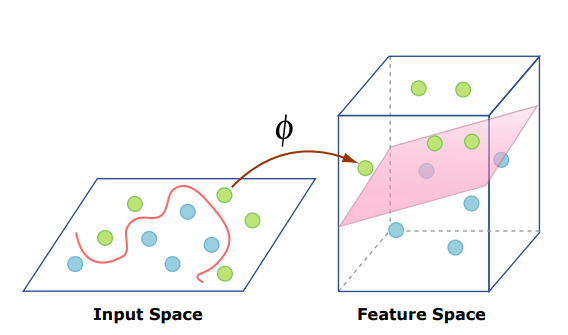
\includegraphics[scale=0.5]{notebooks/ML/img/kernel_trick.png}
    \caption{Kernel Trick}
\end{figure}

El paso fundamental del truco del kernel es que no es necesario conocer el mapeo $\phi$ explícitamente pues por el teorema de \textit{Mercer}
$$
K(x_i , x_j) = \langle \phi(x_i) , \phi(x_j) \rangle
$$
donde $K: X \times X \rightarrow \mathbb{R} $ es un kernel de \textit{Mercer} en un espacio de \textit{Hilbert} (posiblemente de dimensión infinita), por lo que solo basta que definamos $K$ para tener un posible mapeo de las características. 

\subsection{Kernels}

Para que un kernel pueda utilizarse en el contexto de las SVM, es importante que cumpla con las condiciones de \textit{Mercer}: 
\begin{itemize}
    \item Symmetry: $K(x,y) = K(y,x) \quad \forall x,y$ 
    \item Positive Semi-Definiteness: Para cualquier vector $c \in \mathbb{R}^n$, y $x_1 , \dots x_n$ una cantidad finita de puntos, se debe satisfacer que  
    $$\sum_{ij}c_ix_jK(x_i,x_j) \geq 0$$
\end{itemize}

Algunos ejemplos de \textit{kernels} que se pueden utilizar son: 

\begin{enumerate}
    \item \textbf{Linear Kernel}: $K(x,y) = \langle x , y \rangle$. 
    
    El más útil cuando la data es linealmente separable. 
    \item \textbf{Polynomial Kernel}: $K(x,y) = (x^{\top}y + c)^d$. 
    
    El parámetro $d$ controla el nivel de complejidad del kernel pero valores muy altos podrían llevar a overfitting.
    \item \textbf{Gaussian Radial Basis Function (RBF) Kernel}: $K(x,y) = e^{-\gamma||x-y||^2}$. 
    
    Este kernel es el más popular pues \textbf{mapea los datos a un espacio de dimensión infinita}. El parámetro $\gamma$ controla la complejidad de los \textit{decision boundaries} al agregar mayor o menor spread al kernel. 
    \item \textbf{Sigmoid Kernel}: $K(x,y) = \text{tanh}(ax^{\top}y + b)$
\end{enumerate}

\begin{figure}[H]
    \center
    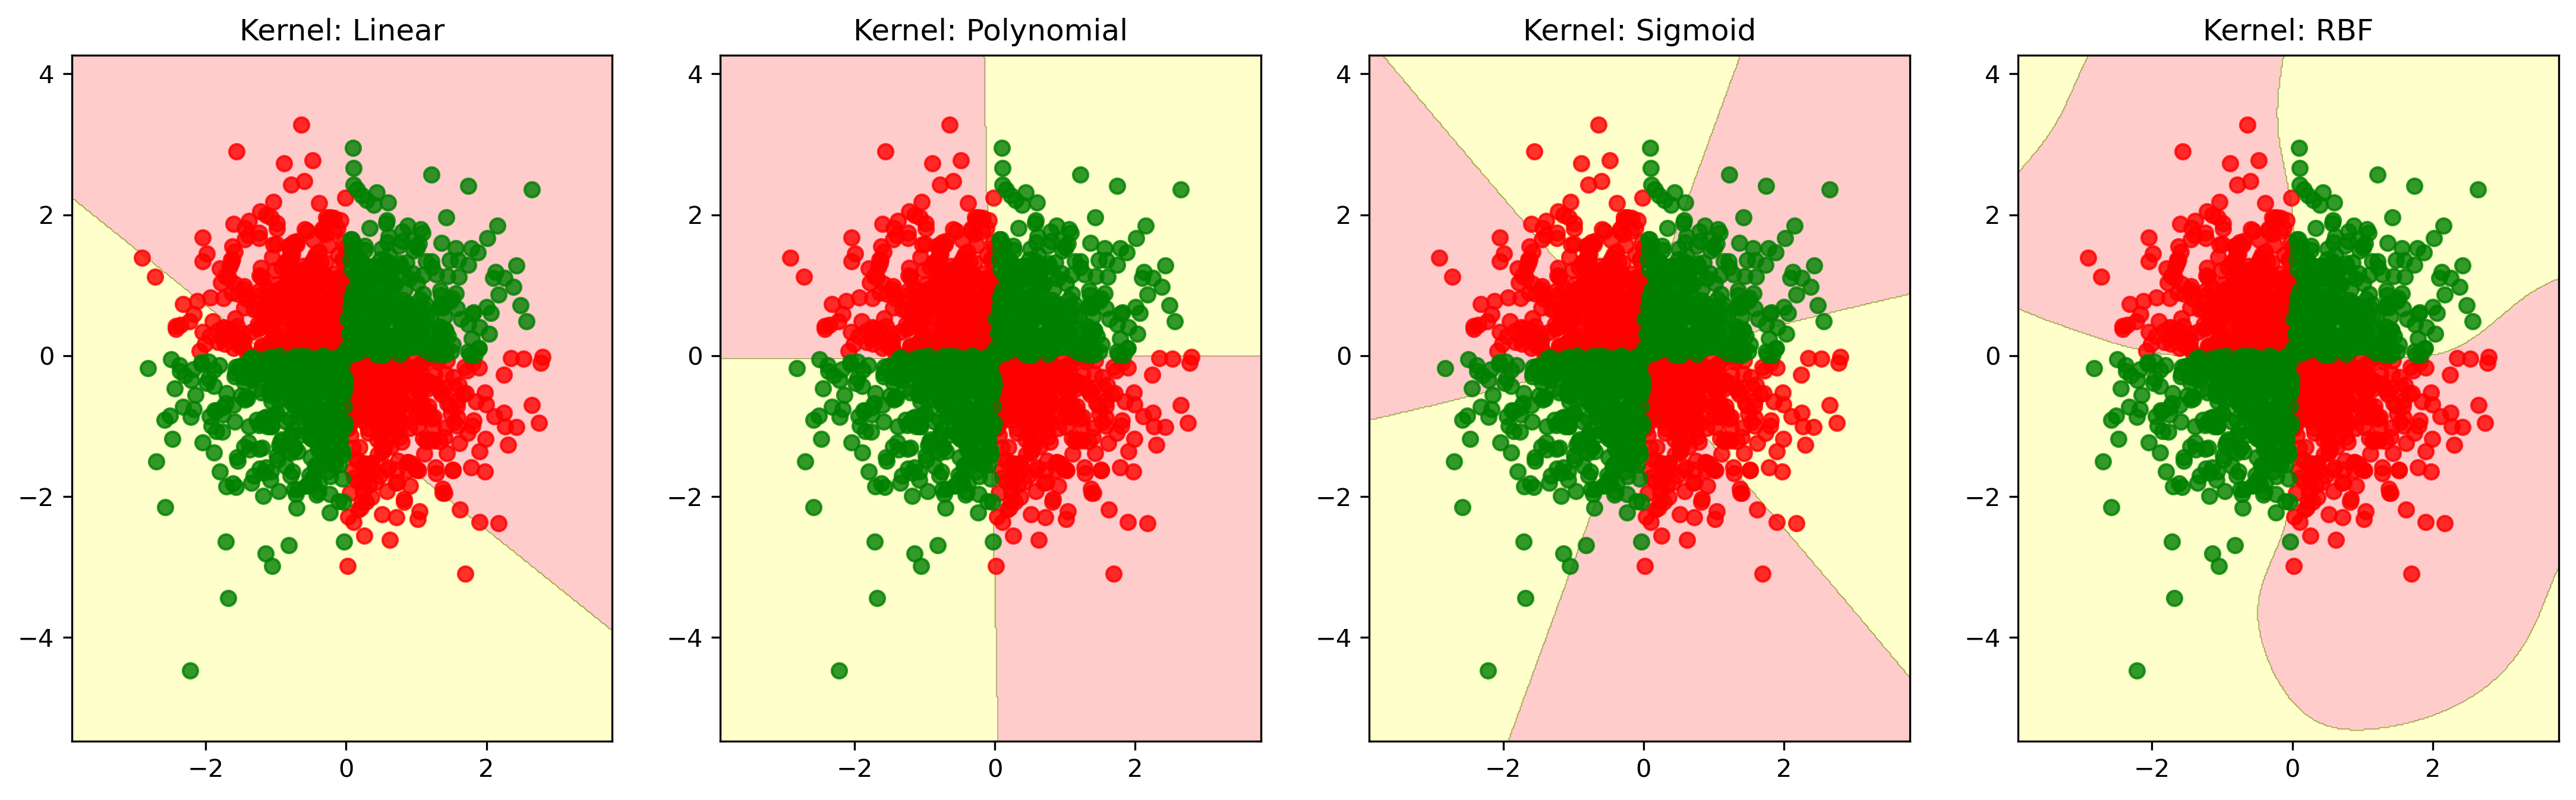
\includegraphics[scale=0.35]{notebooks/ML/img/kernel_decision_boundaries.png}
    \caption{Kernel Decision Boundaries}
\end{figure}

\section{ARIMA}

ARIMA es la abreviación de \textit{Auto-Regressive Integrated Moving Average} y es un método estadístico para realizar forecasting sobre series de tiempo que integra los siguientes conceptos:

\begin{enumerate}
    \item Toma en consideración patrones de crecimiento/decrecimiento en la serie de tiempo (\textit{Auto-Regressive}). 
    \item Estima tasa de crecimiento/decrecimiento (\textit{Integrated}).
    \item Controla el ruido entre datos consecutivos en el tiempo (\textit{Moving Average}).
\end{enumerate}

La fórmula general para este tipo de modelos viene dada por 
$$
Y_t = c + \phi_1y^d_{t-1} + \dots + \phi_py^d_{t-p} + \theta_1e_{t-1} + \dots + \theta_q e_{t-q} + e_t
$$
Aquí $c$ es una constante y $e$ es un término de error. Los modelos de este tipo son escritos como ARIMA($p,d,q$) donde: 

\begin{itemize}
    \item $p$ es la cantidad de tiempos en que la variable es mirada al pasado (Lag).
    \item $d$ es la cantidad de veces que la variable es diferenciada para producir una señal estacionaria. $d=0$ refiere a que la señal ya es estacionaria, $d=1$ es que la señal crece/decrece linealmente y $d=2$ es que la señal crece exponencialmente. 
    \item $q$ representa la cantidad de lag para el término de error $e$, esto captura el \textit{Moving Average}.
\end{itemize}

\subsection{P Value}

En la práctica, es posible determinar el valor de $p$ a través del \textit{Partial Autocorrelation Plot}. Este gráfico muestra la relación de un valor en la serie de tiempo con \textbf{un solo lag} (eliminando relaciones de tiempos intermedios ajustando una regresión lineal y quedándose sólo con el parámetro correspondiente).
\begin{figure}[H]
    \center
    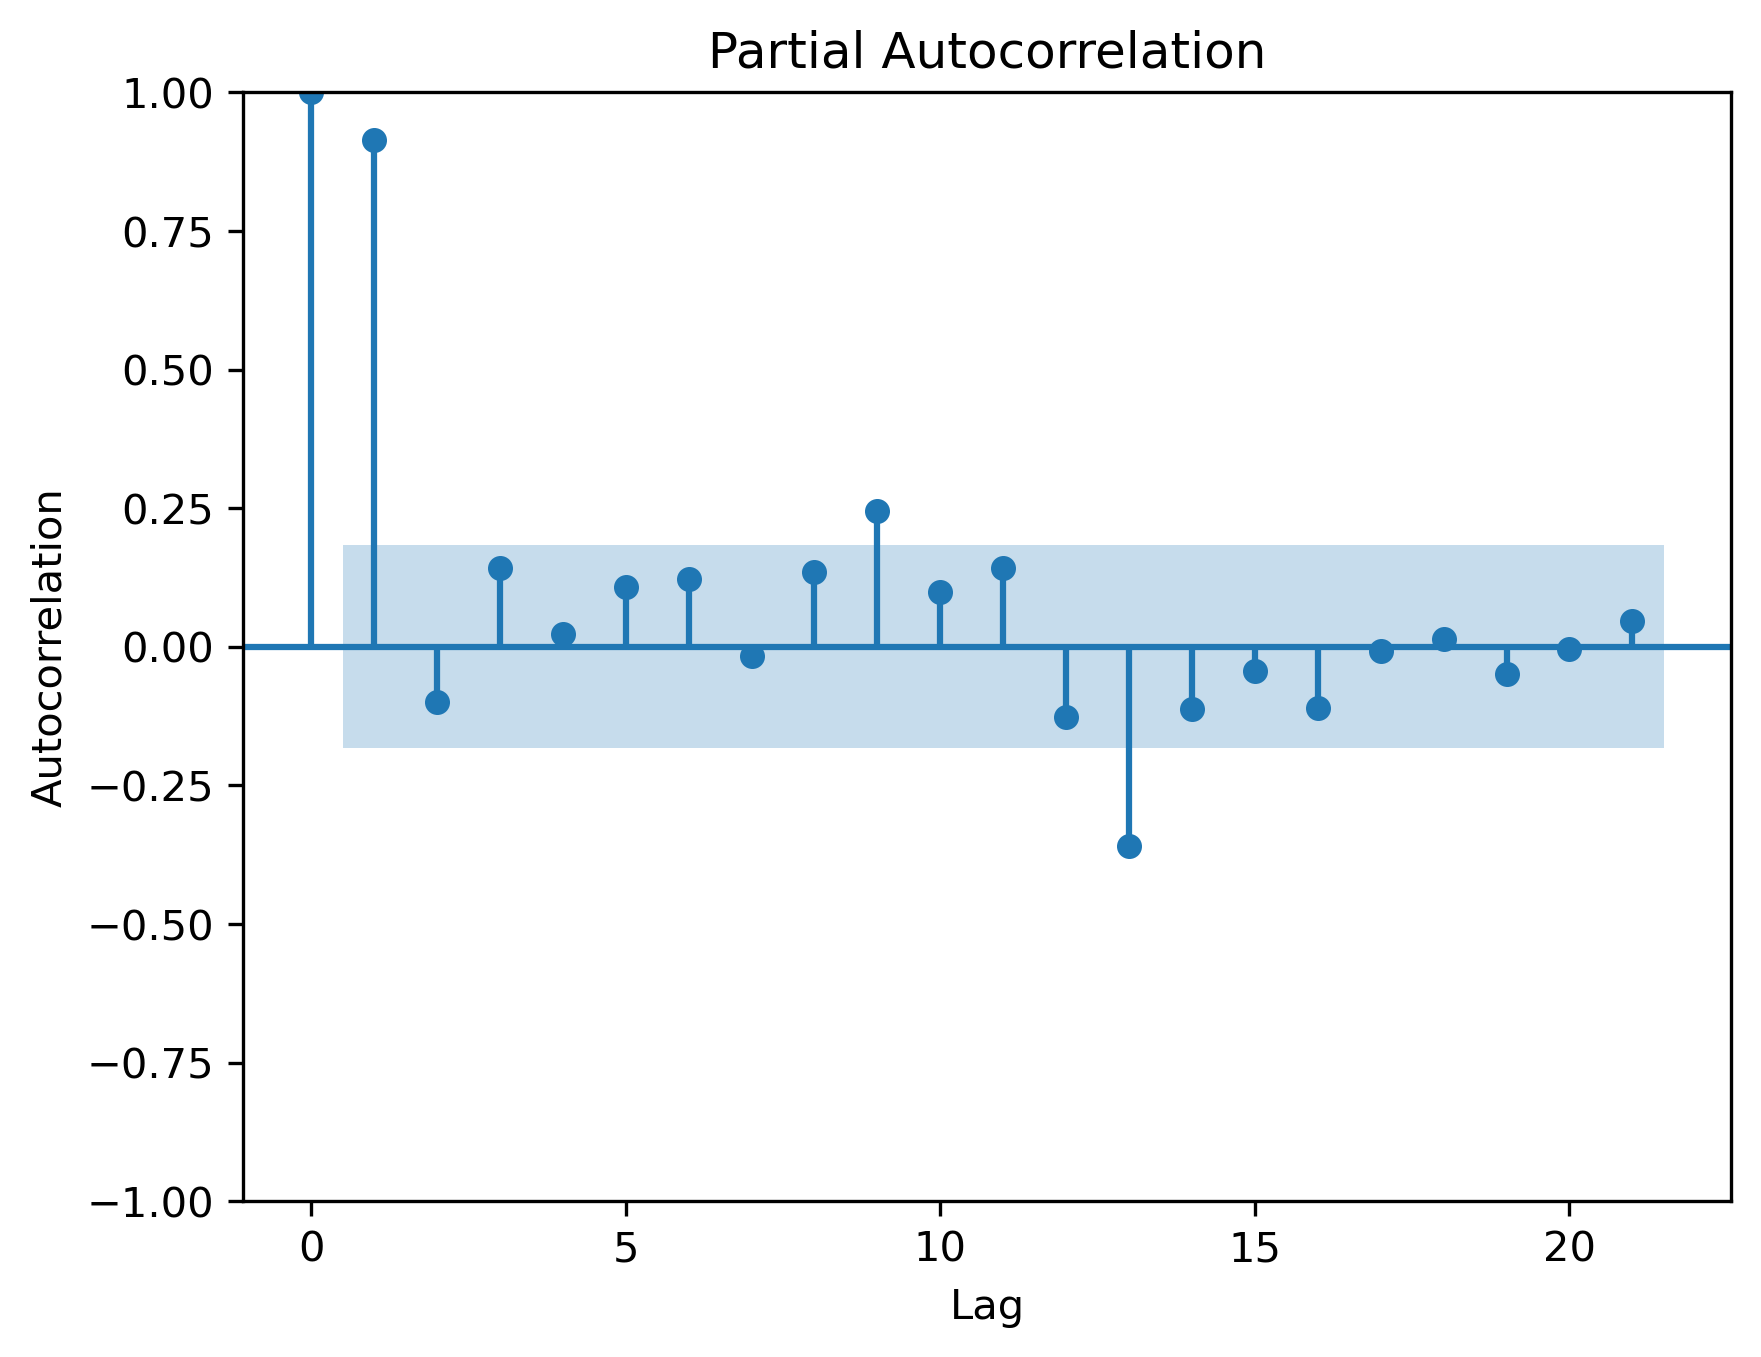
\includegraphics[scale=0.5]{notebooks/TS/img/partial_autocorrelation.png}
    \caption{Partial Autocorrelation Plot}
\end{figure}
El valor óptimo es el último punto después del cual todos los lags están dentro de las bandas azules (intervalos de confianza), en este caso $p=13$. 

\subsection{D Value}

El valor de $d$ se puede calcular diferenciando la serie de tiempo hasta encontrar una serie estacionaria. Esto lo podemos medir con un test estadístico de estacionalidad (\textit{Augmented Dickey Fuller Test}).

\begin{figure}[H]
    \center
    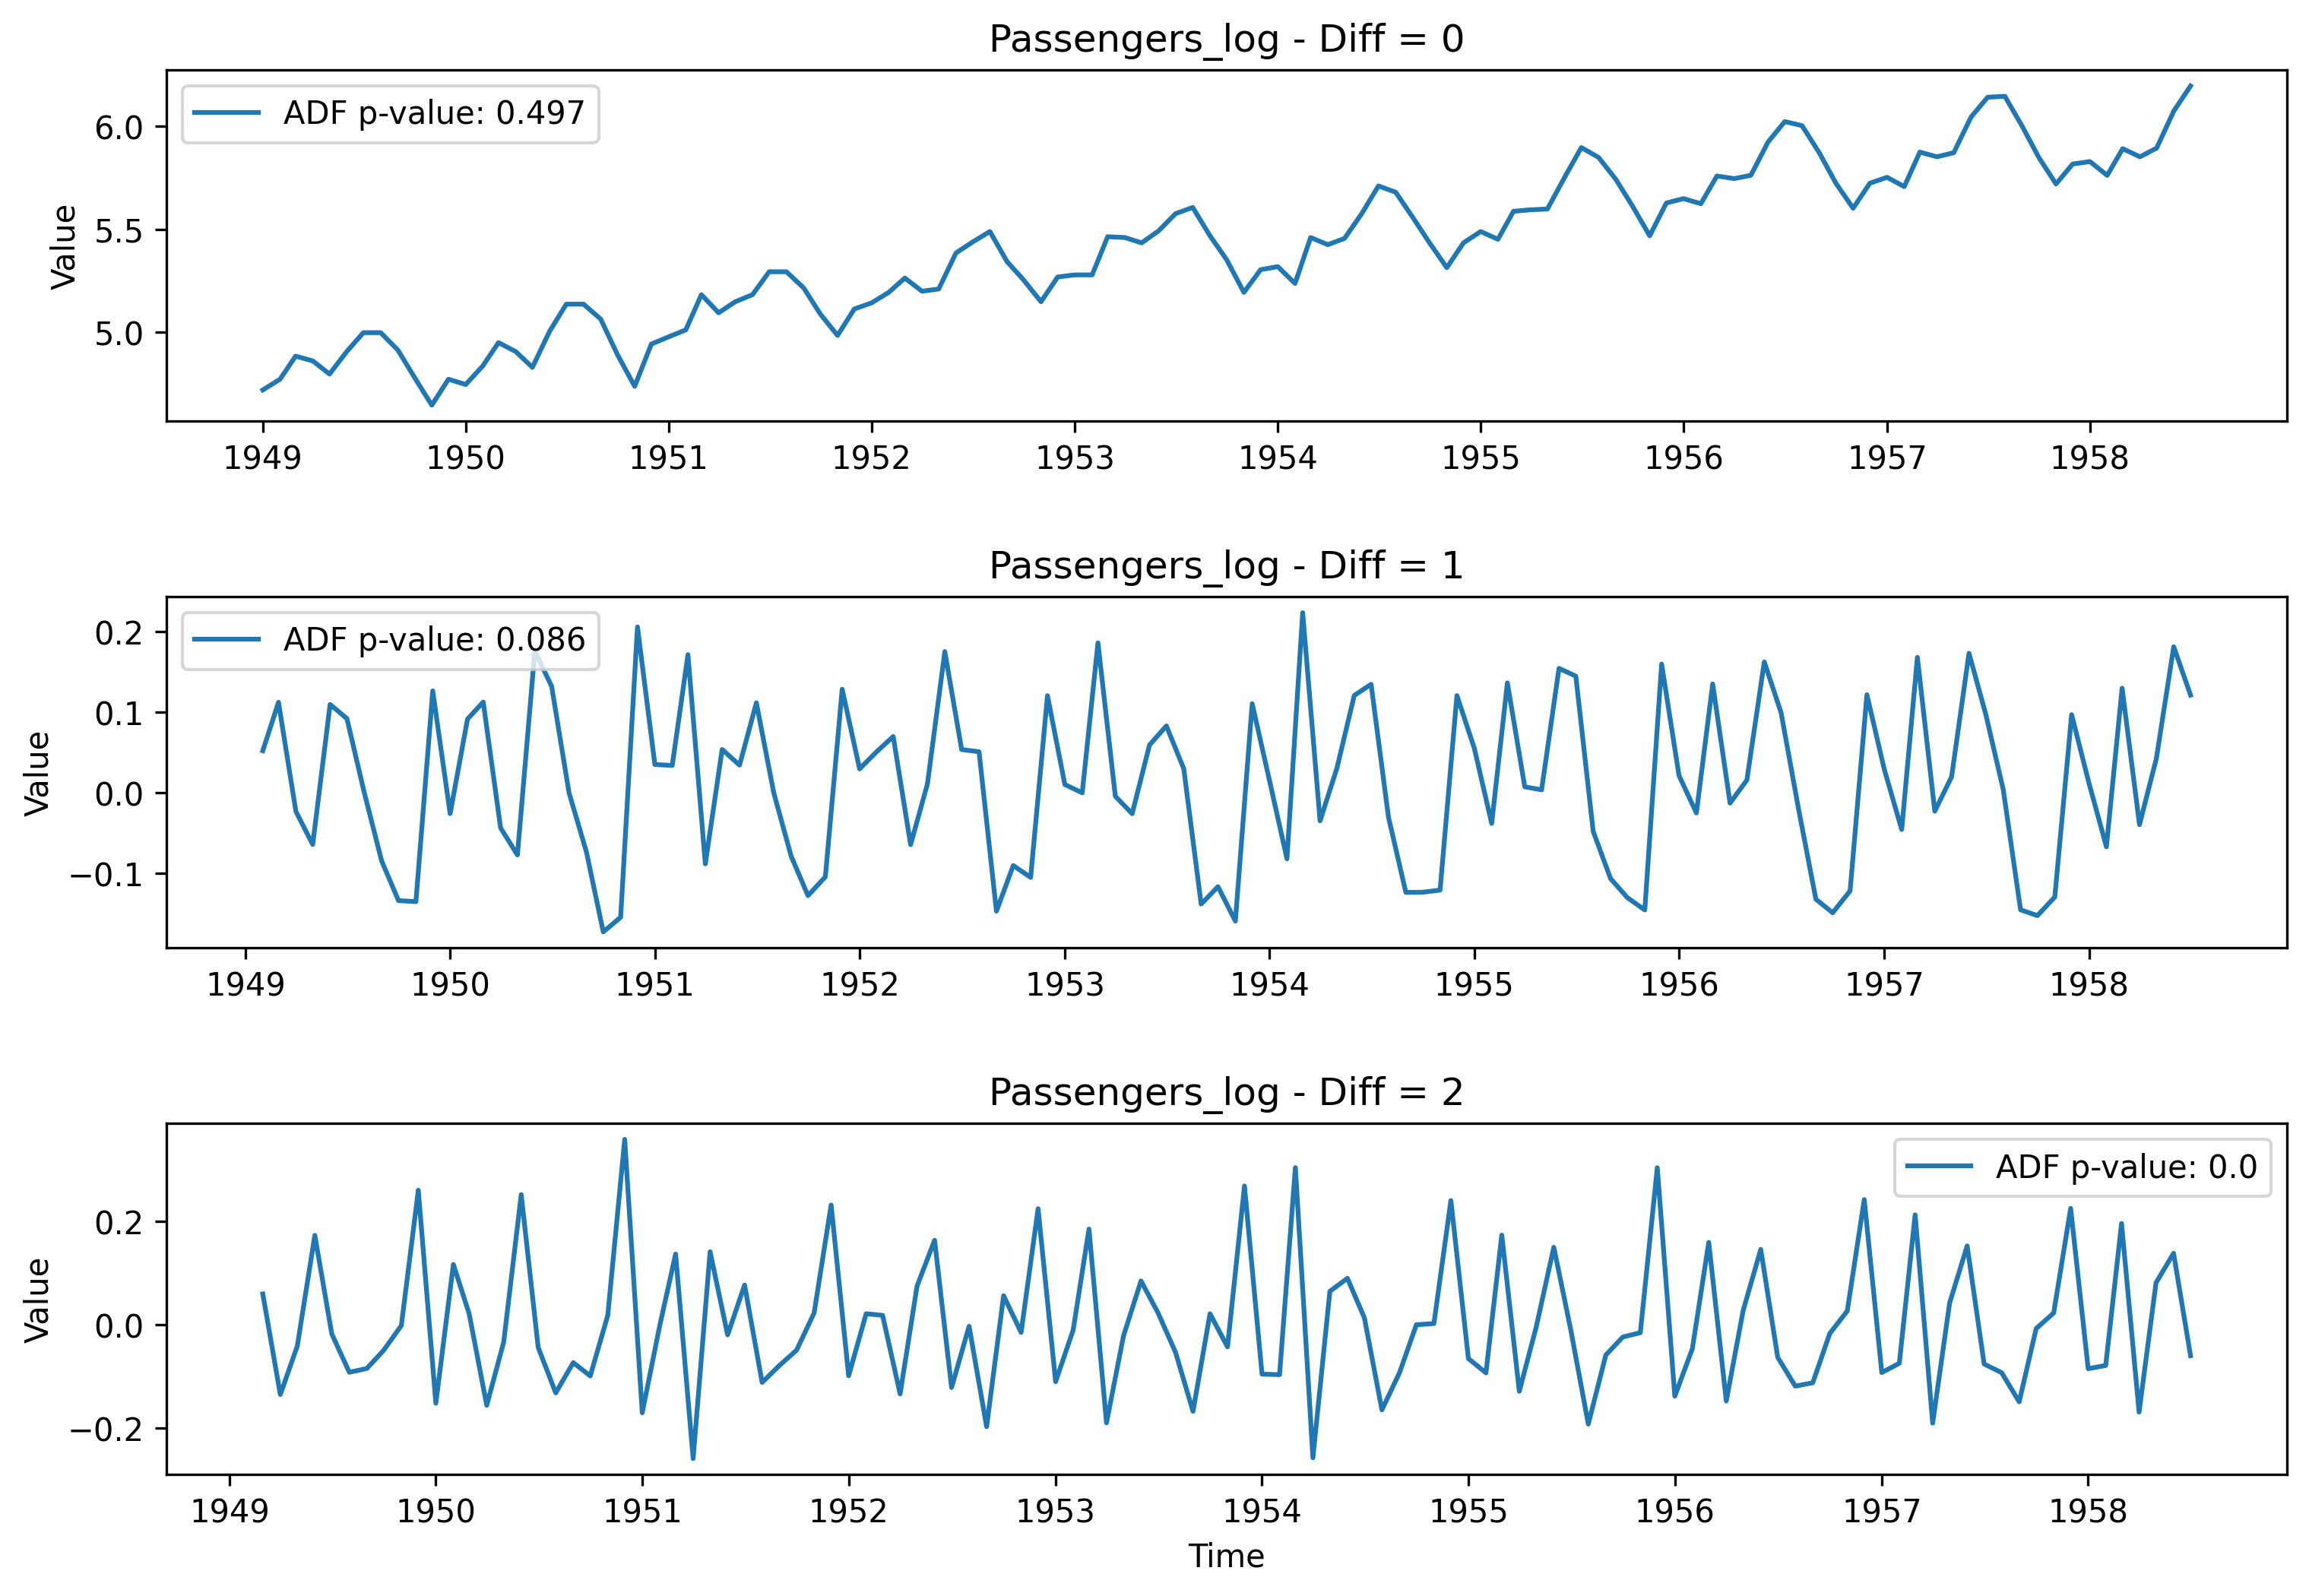
\includegraphics[scale=0.5]{notebooks/TS/img/time_series_differentiation.png}
    \caption{Time Series Differentiation Plot}
\end{figure}

Vemos que el $p$-valor en la segunda diferenciación ya es lo suficientemente pequeño para asumir estacionalidad en la serie de tiempo, así $d=2$. 

\subsection{Q Value}
Finalmente, para determinar el valor $q$ es posible ver el \textit{Autocorrelation Plot} que muestra la relación de un valor en la serie de tiempo con \textbf{todos los $p$ lags} anteriores. 
\begin{figure}[H]
    \center
    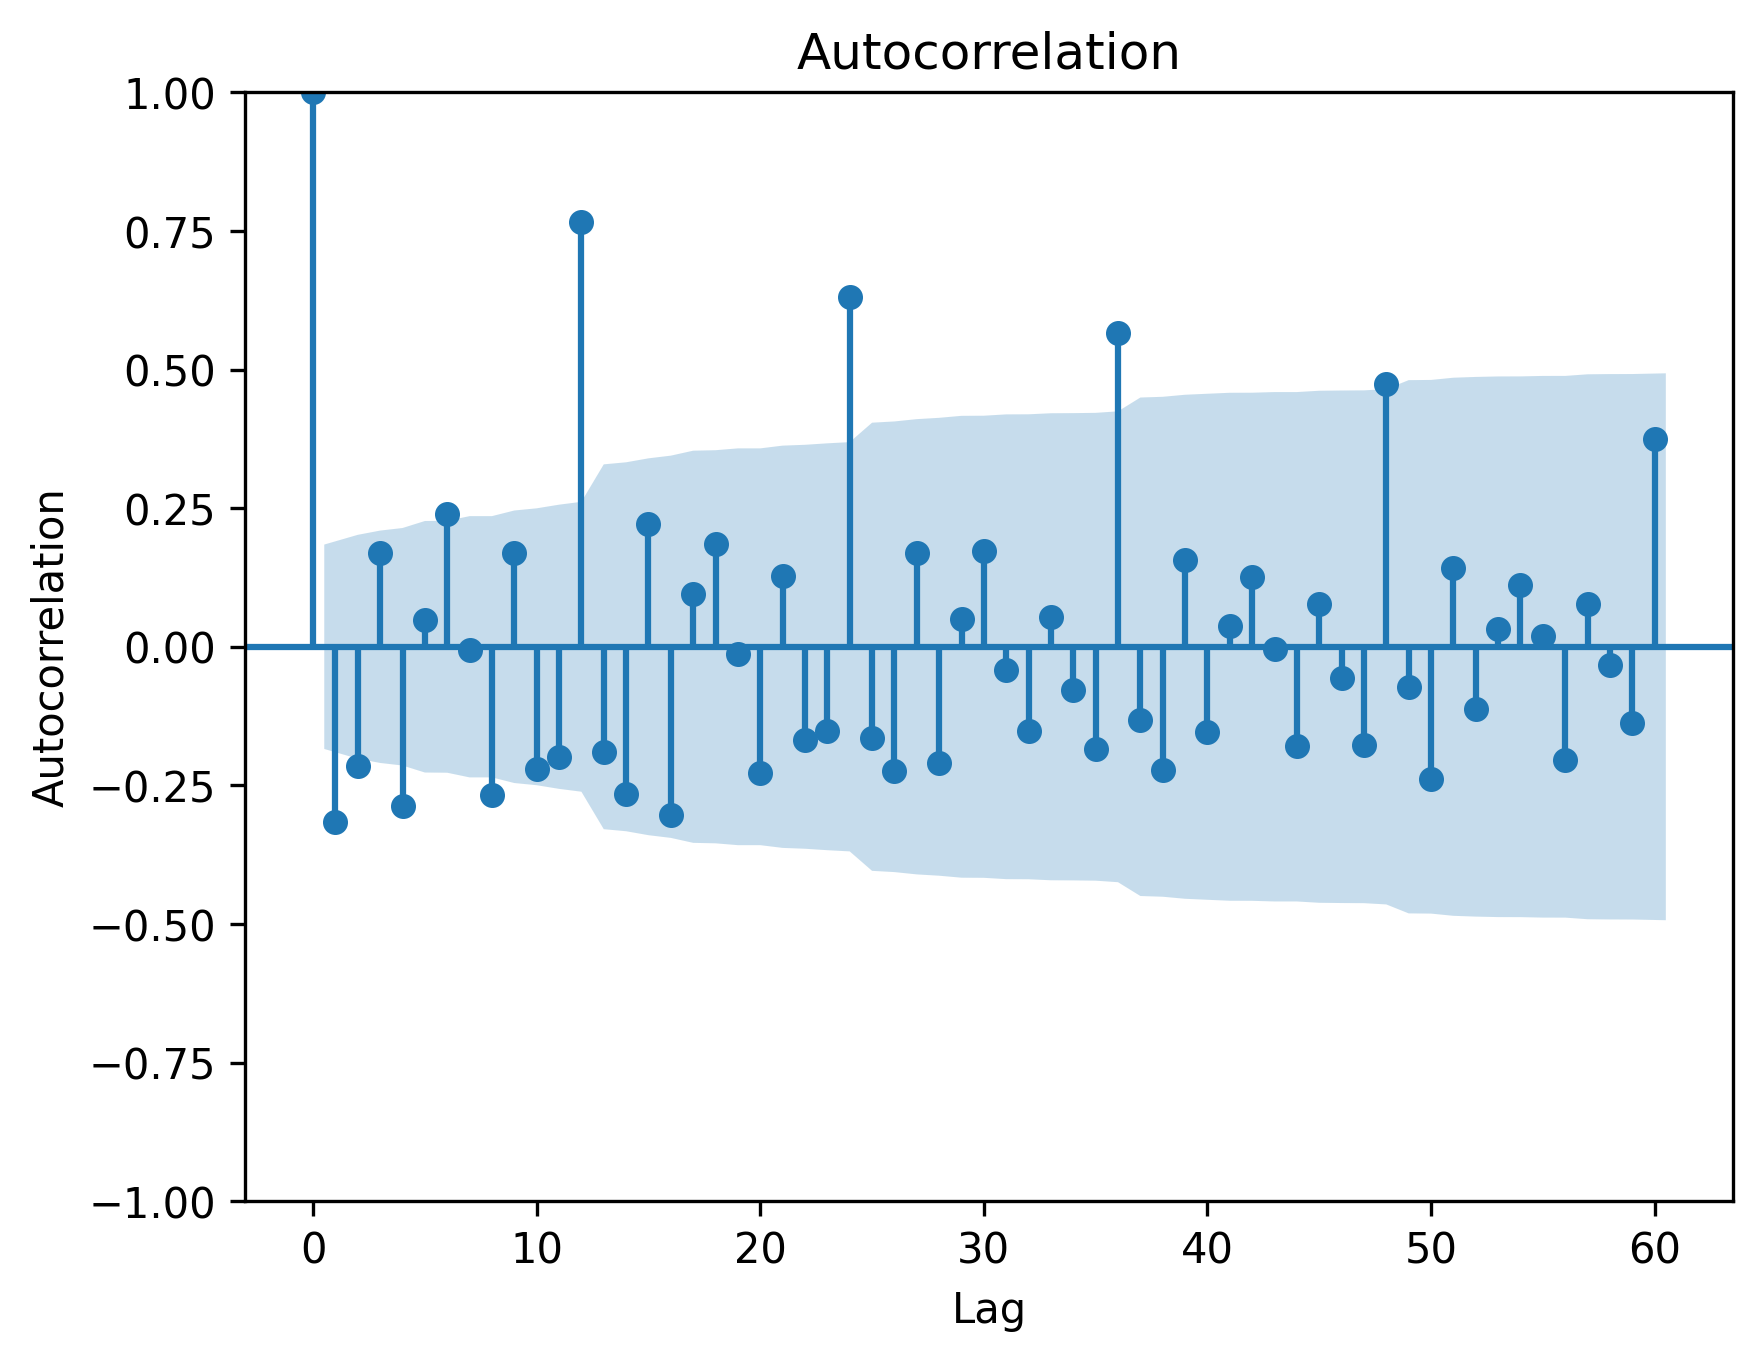
\includegraphics[scale=0.5]{notebooks/TS/img/autocorrelation.png}
    \caption{Autocorrelation Plot}
\end{figure}
En este caso, el último valor anterior a que todos los lag caigan en la zona azul, es $q=12$.
\begin{figure}[H]
    \center
    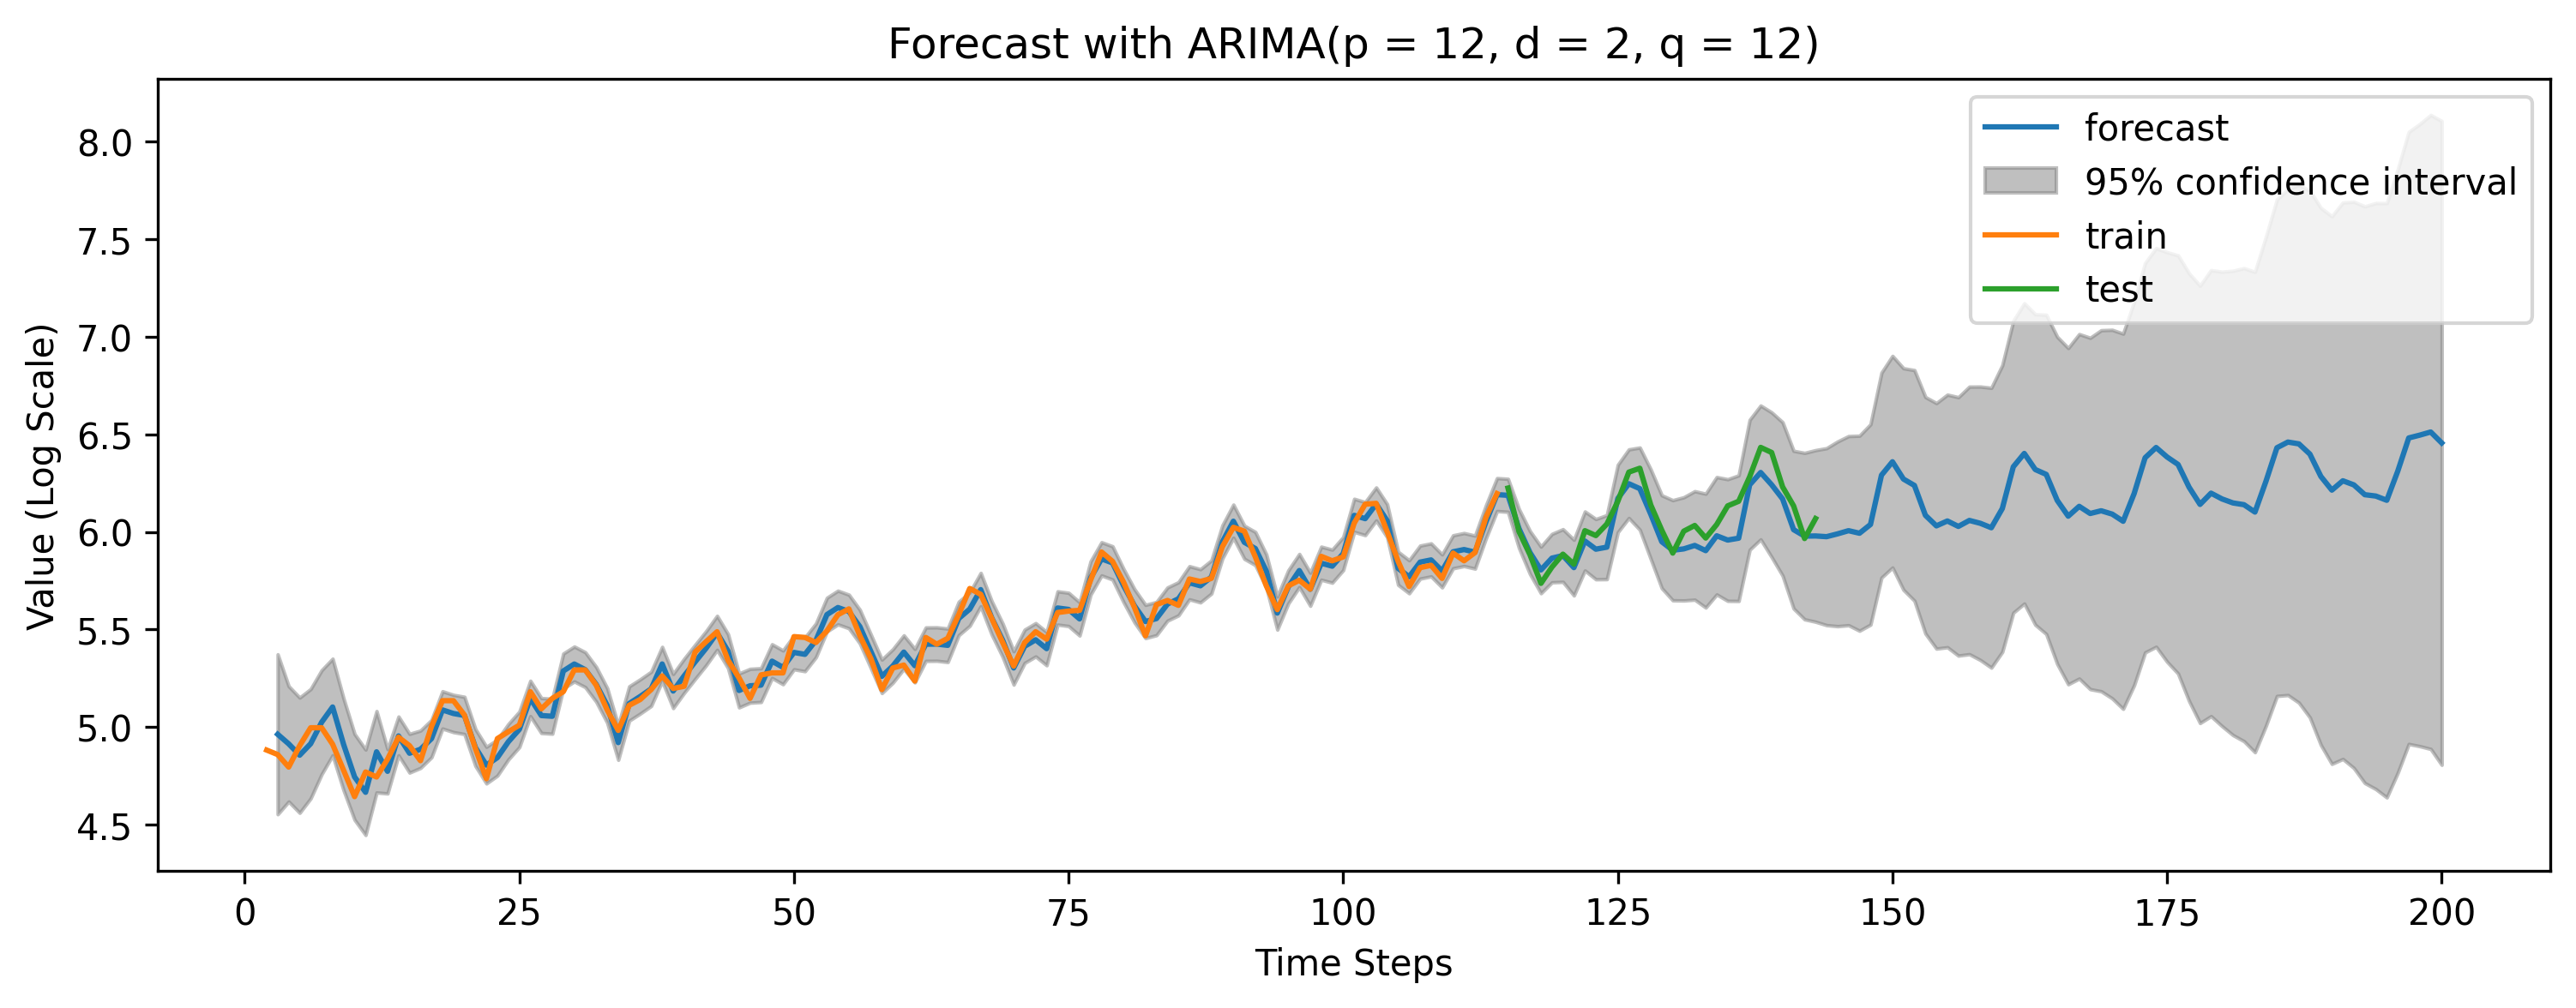
\includegraphics[scale=0.5]{notebooks/TS/img/arima_results.png}
    \caption{ARIMA over Flight Passengers Forecasting}
\end{figure}

\section{K-Means}

El algoritmo de \textit{K-Means} es un algoritmo \textbf{no supervisado de clustering}. 
El objetivo es agrupar los datos alrededor de \textbf{centroides} de tal forma en que se minimice la suma de alguna medida de distancia. Vale decir, encontrar el conjunto $ S = \{ S_1 , \dots, S_k \} $ de clusters ($k$ hiperparámetro) tal que

\begin{equation*}
\begin{aligned}
S = \argmin_{S} \sum_{i=1}^{k}\sum_{x \in S_i}||x- \mu_i||_{2}^2
\end{aligned}
\end{equation*}

Notar que $\mu_i = \frac{1}{|S_i|}\sum_{x \in S_i}x_i$ es el centroide del cluster $S_i$ para todo $i$. El algoritmo que realiza esta búsqueda es el siguiente: 
\begin{enumerate}
    \item Seleccionar $k$ centroides aleatorios del conjunto de datos. 
    \item Asignar cada punto del conjunto de datos al centroide más cercano. 
    \item Actualizar el nuevo centroide del cluster $S_i$ según $\mu_i = \frac{1}{|S_i|}\sum_{x \in S_i}x_i$. Iterar los pasos 2 y 3 hasta que la asignación no cambie.
\end{enumerate}

\begin{figure}[H]
    \center
    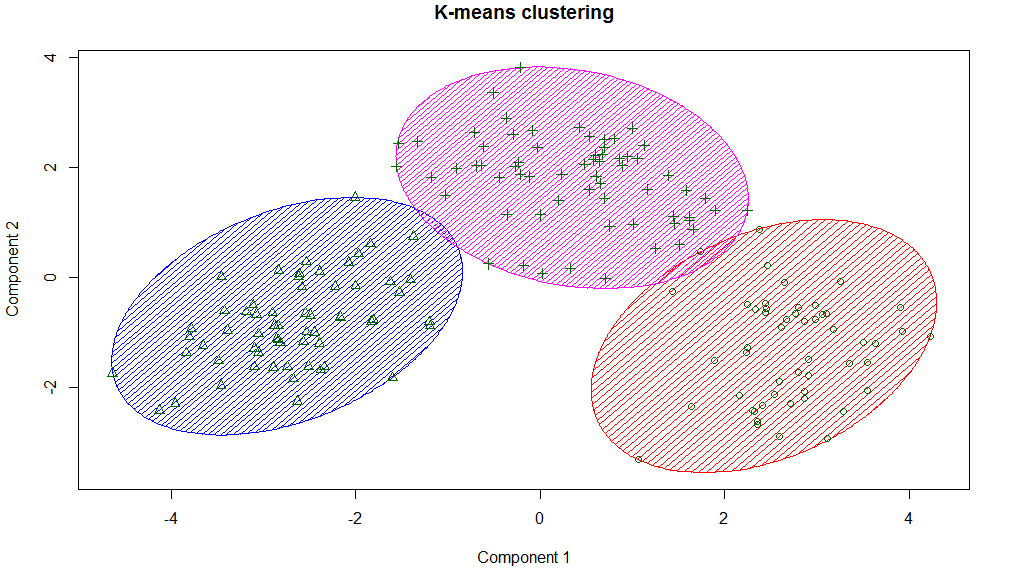
\includegraphics[scale=0.25]{notebooks/ML/img/k_means_diagram.png}
    \caption{K-Means Diagram}
\end{figure}

\textbf{Este algoritmo siempre converge pero no asegura el óptimo global}. Además, la distancia euclidiana asume que los clusters tienen \textbf{forma esférica}. Por último, es muy \textbf{sensible a outliers}

La selección del hiper-parámetro $k$ se puede hacer utilizando el método del codo (\textit{Elbow Method}). Es decir, calcular el error de la función objetivo para distintos valores de $k$ y seleccionar el menor valor de $k$ tal que la función objetivo no cambie en gran magnitud con los valores siguientes. 

\begin{figure}[H]
    \center
    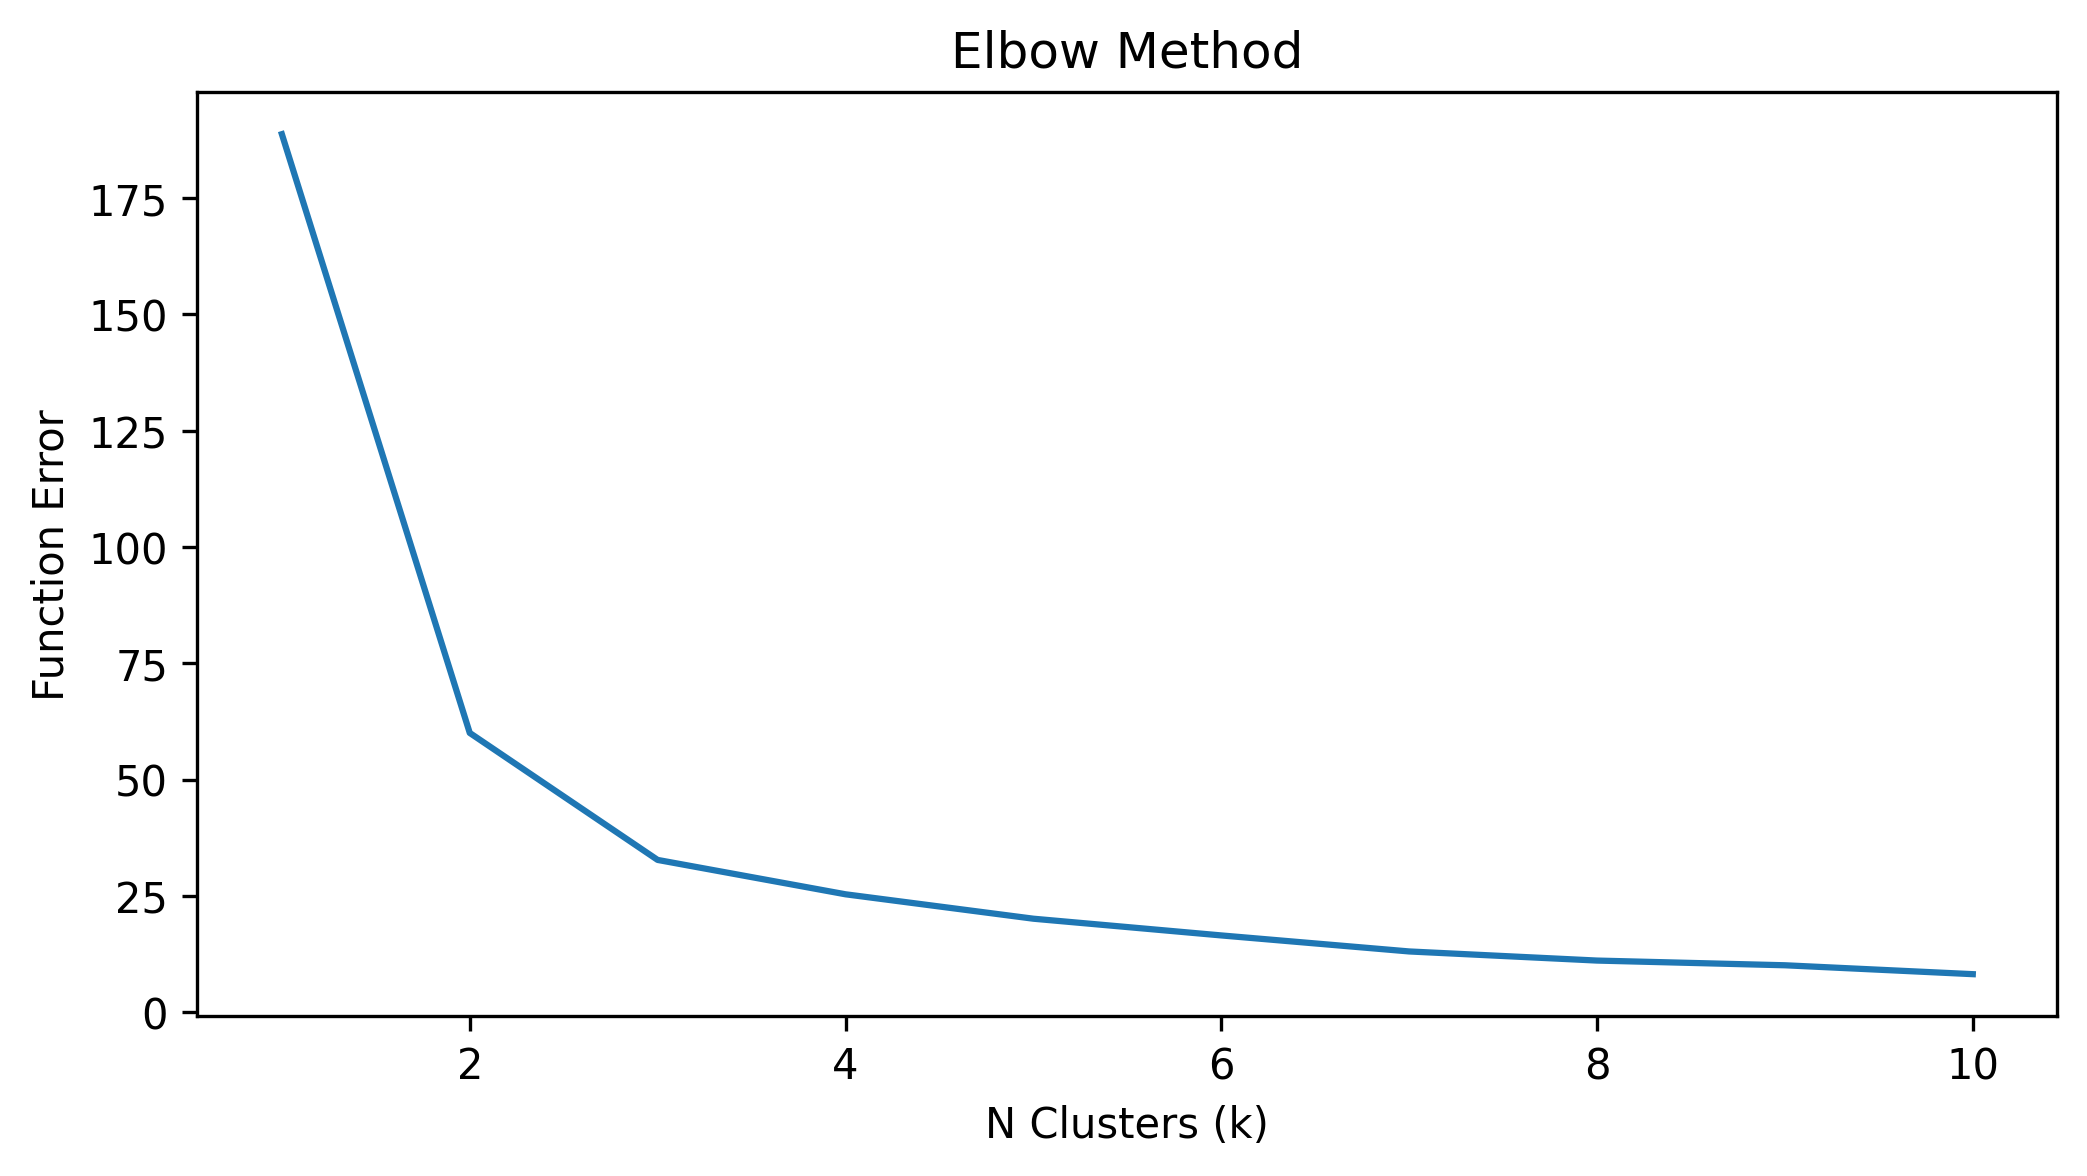
\includegraphics[scale=0.45]{notebooks/ML/img/elbow_method_k_means.png}
    \caption{Elbow Method}
\end{figure}

En este ejemplo, el valor óptimo de clusters con el \textit{Elbow Method} es $k=3$.  

\section{Hierarchical Clustering}

Los algoritmos de \textit{Hierarchical Clustering} buscan crear jerarquías de grupos conformados por elementos del dataset. Estos pueden ser de 2 categorías: 

\begin{enumerate}
    \item \textbf{Agglomerative}: Cada observación comienza en un grupo y comienzan a juntarse. 
    \item \textbf{Divisive}: Comenzar de un grupo y empezar a dividir.
\end{enumerate}

\begin{figure}[H]
    \center
    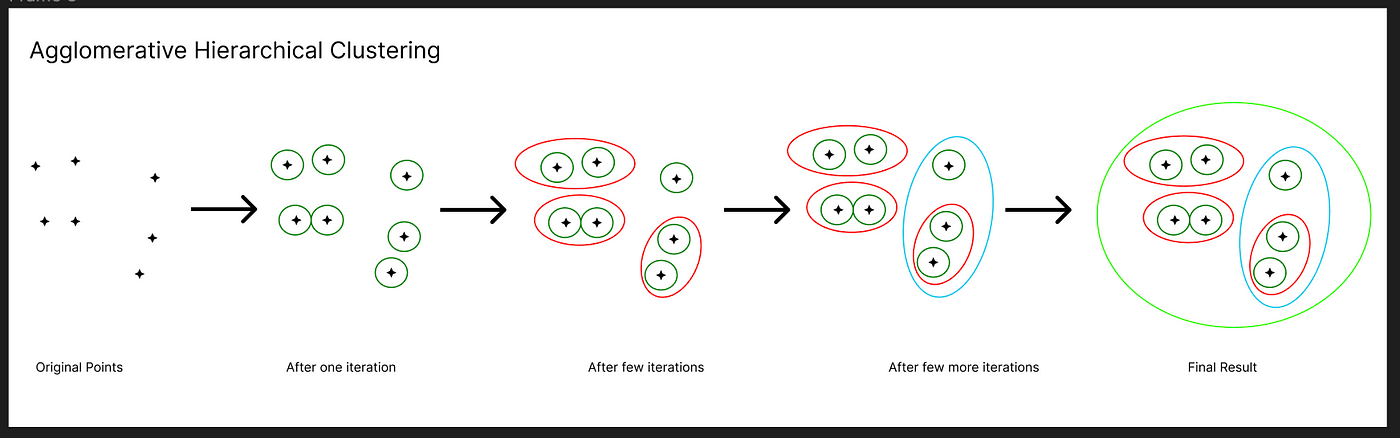
\includegraphics[scale=0.25]{notebooks/ML/img/agg_clustering.png}
    \caption{Agglomerative Clustering Example}
\end{figure}

En el caso aglomerativo, los clusters más cercanos se juntan para formar un nuevo grupo. Existen distintos criterios para definir cercanía: 

\begin{itemize}
    \item \textbf{Single}: Los elementos más cercanos entre clusters. $$\min_{a \in A, b \in B} d(a,b)$$
    \item \textbf{Complete}: Los elementos más alejados entre clusters.  $$\max_{a \in A, b \in B} d(a,b)$$
    \item \textbf{Average}: La distancia promedio entre todos los puntos de ambos clusters. $$\frac{1}{|A| \cdot |B|}\sum_{a \in A} \sum_{b \in B} d(a,b)$$
    \item \textbf{Ward}: Minimizar la varianza entre clusters luego de la unión. 
    $$\frac{|A|\cdot|B|}{|A \cup B|}||\mu_A - \mu_B||^2 = \sum_{x \in A \cup B}||x - \mu_{A \cup B}||^2 - \sum_{x \in A}||x - \mu_{A}||^2 - \sum_{x \in B}||x - \mu_{B}||^2$$
\end{itemize}

Estas divisiones se pueden visualizar a través de \textbf{Dendogramas} y cada criterio cambiará la forma de definir los clusters.

\begin{figure}[H]
    \center
    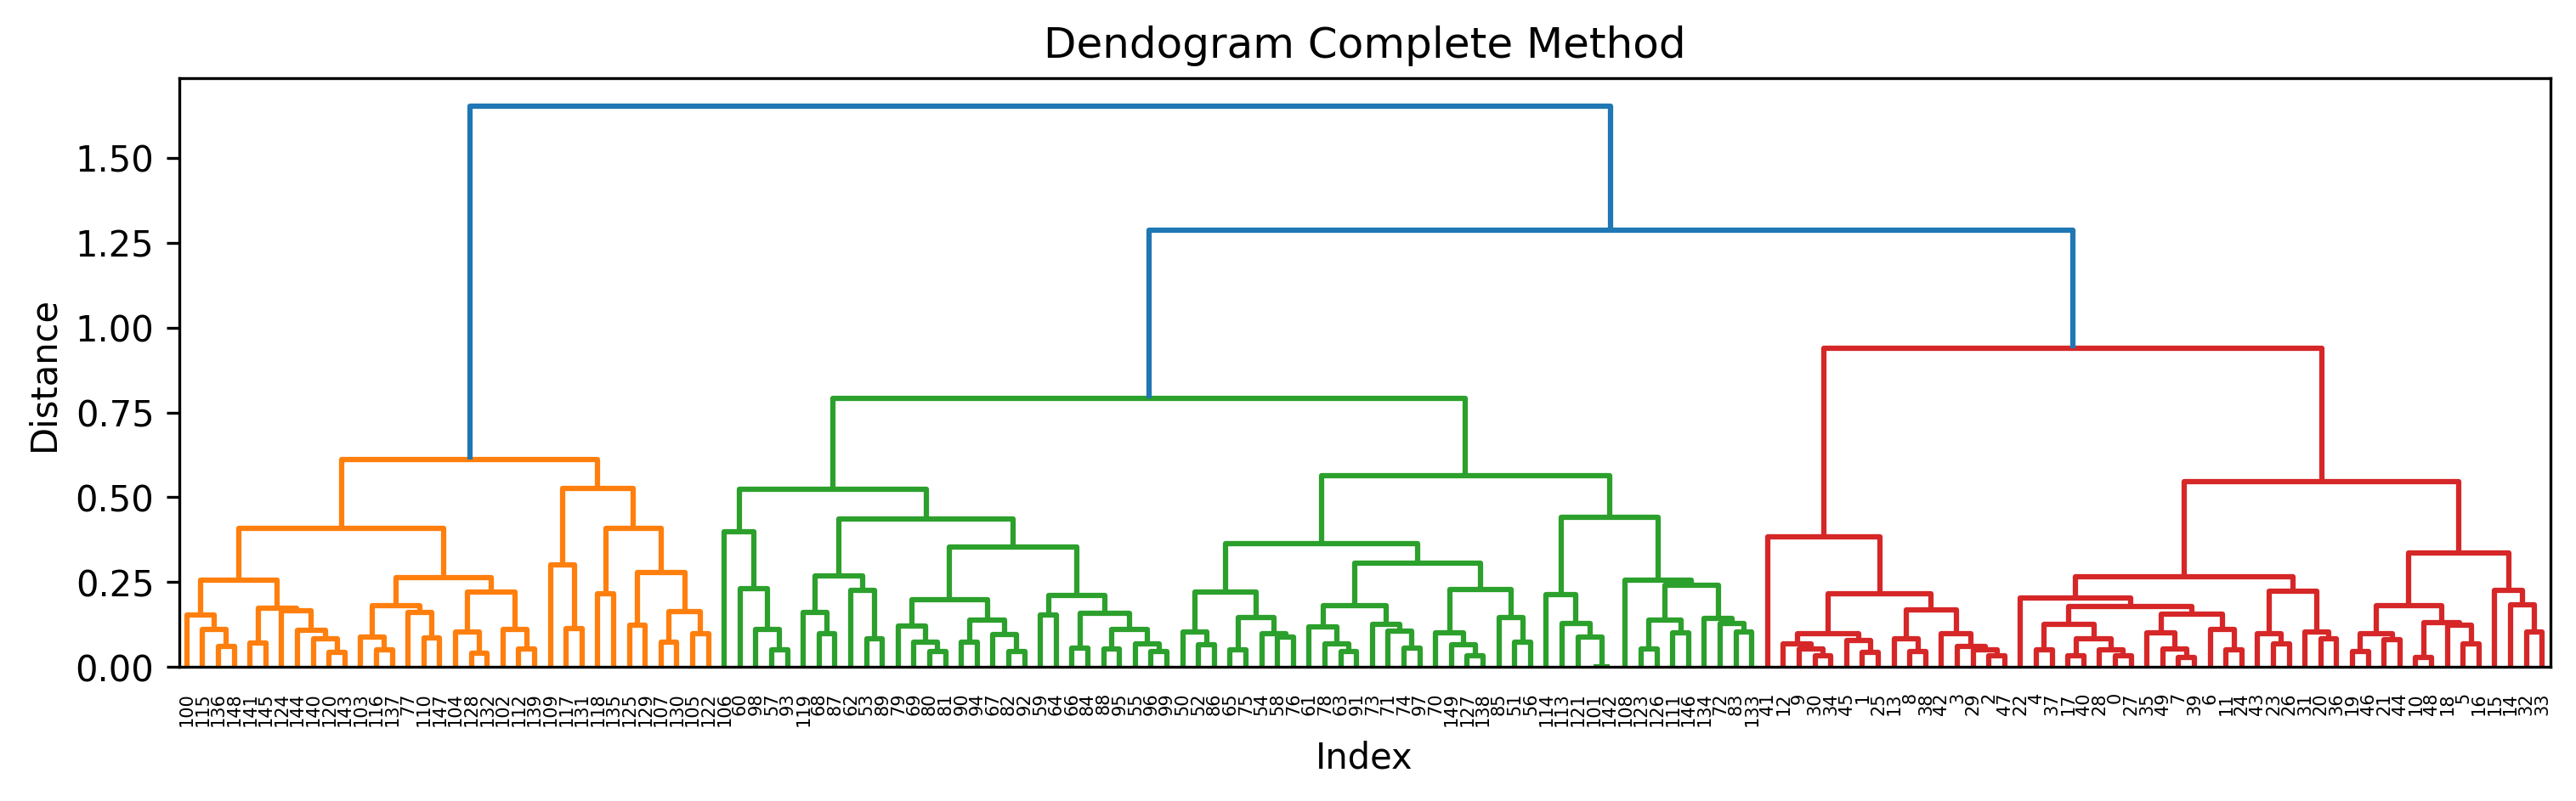
\includegraphics[scale=0.5]{notebooks/ML/img/complete_dendogram_iris.png}
    \caption{Complete Dendogram over Iris Dataset}
\end{figure}

\begin{figure}[H]
    \center
    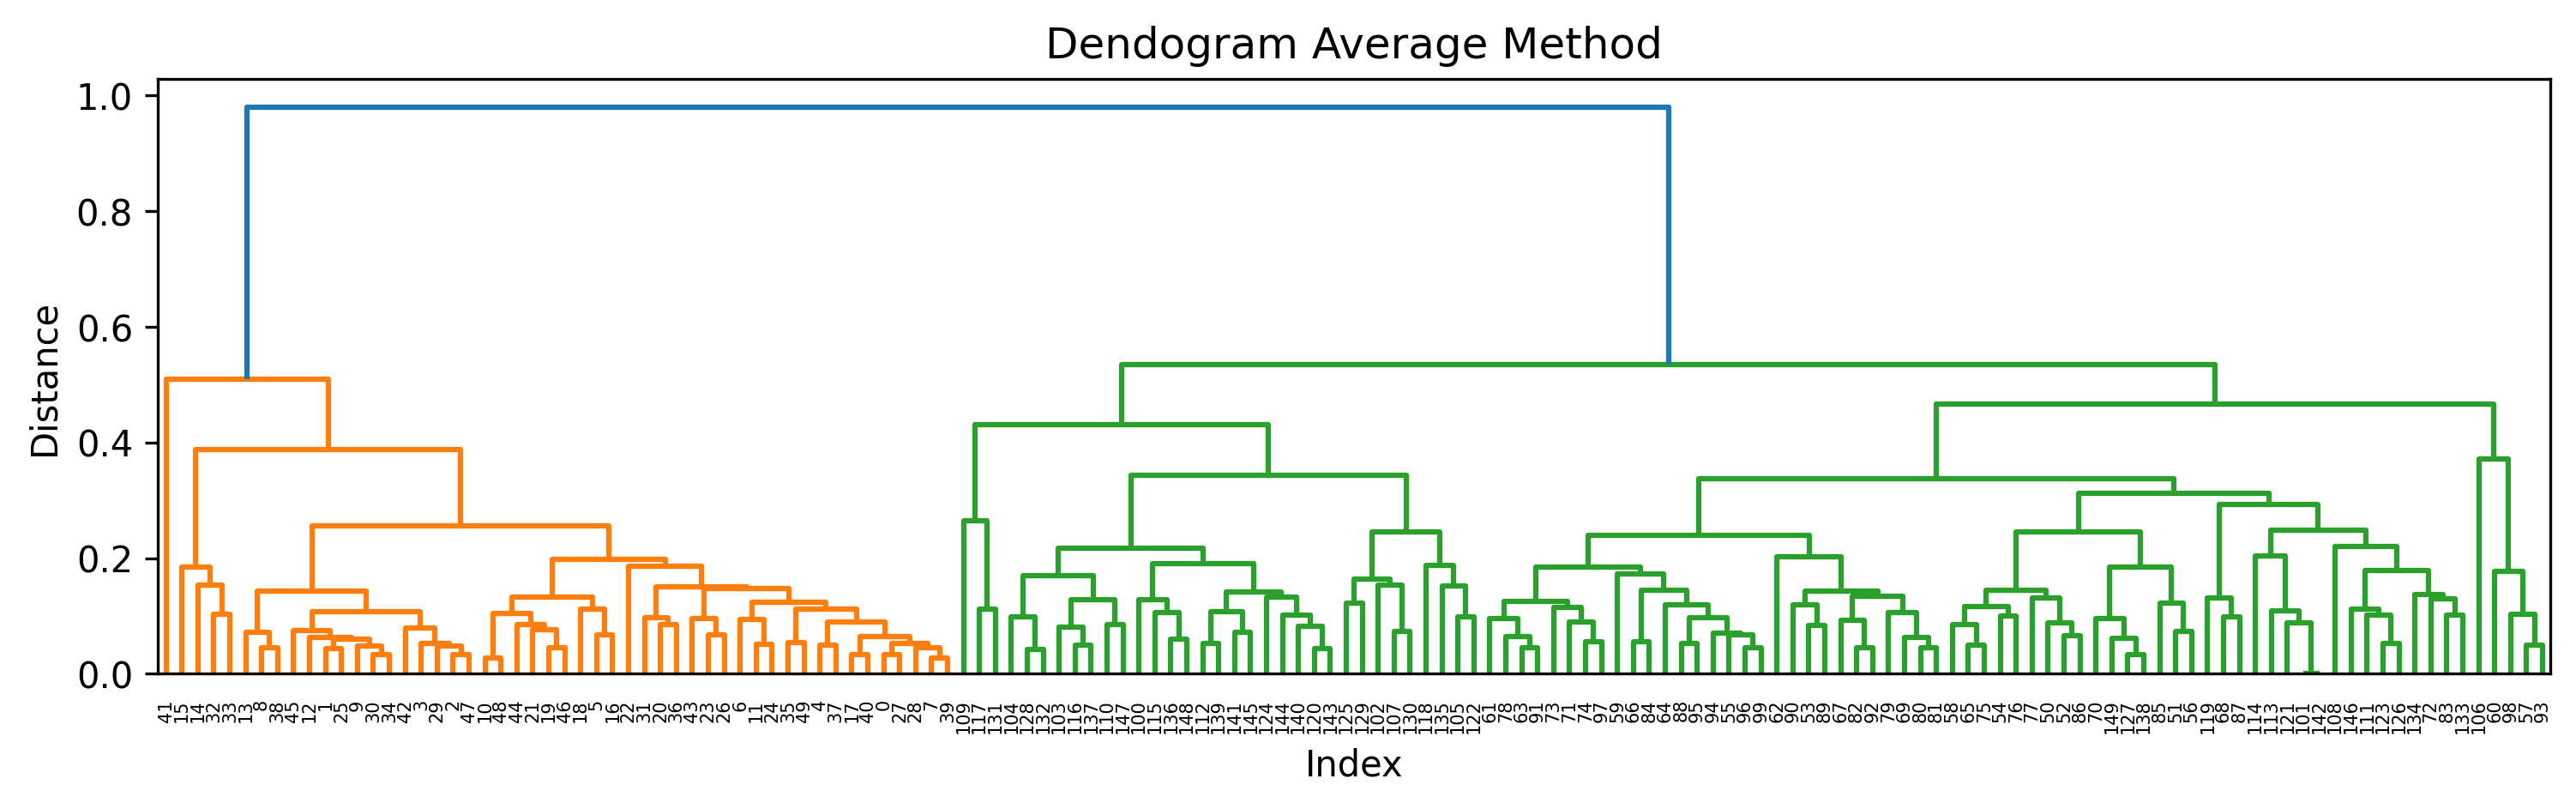
\includegraphics[scale=0.5]{notebooks/ML/img/average_dendogram_iris.png}
    \caption{Average Dendogram over Iris Dataset}
\end{figure}

\section{DBSCAN}

El algoritmo DBSCAN (\textit{Density-based spatial clustering of applications with noise}) es un algoritmo basado en densidad que permite resolver problemas de \textbf{clustering} y realizar \textbf{outlier detection}. 

\begin{figure}[H]
    \center
    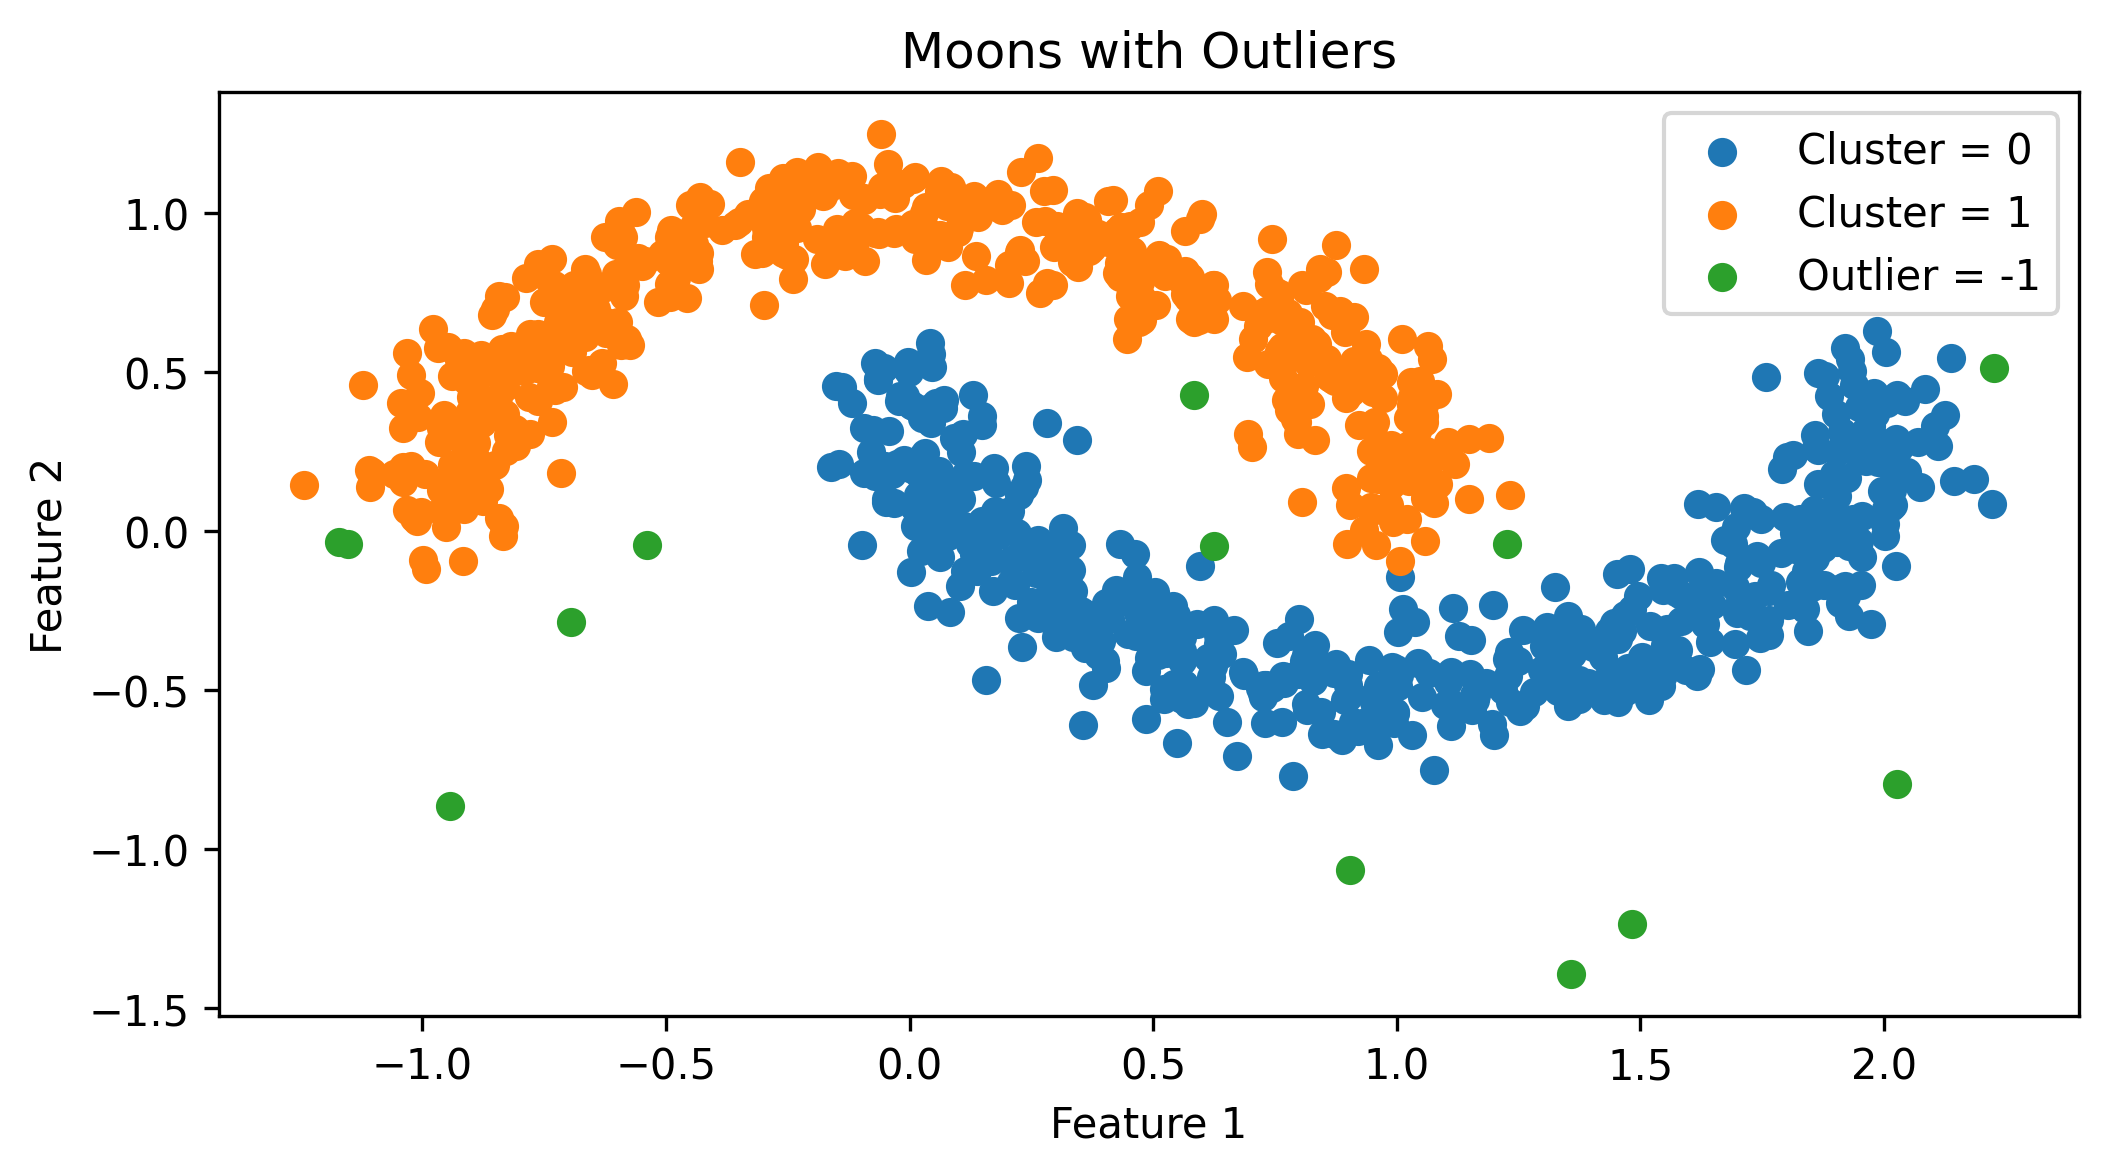
\includegraphics[scale=0.5]{notebooks/ML/img/dbscan_on_moons.png}
    \caption{DBSCAN Example}
\end{figure}

Para realizar esto, se siguen los siguientes pasos: 

\begin{enumerate}
    \item Encontrar todos aquellos puntos (\textit{core points}) que tengan más de \textit{MinNeighbor} vecinos a distancia menor de $\epsilon$. 
    \item Todos los \textit{core points} conexos serán asignados a un cluster. 
    \item Todos los \textit{non core points} serán asignados al cluster del \textit{core point} más cercano. El resto será considerado como \textit{outliers}. 
\end{enumerate}

Sea $C = \{ C_1 , \dots , C_{k} \}$ el número de clusters generados, el algoritmo anterior asegura la optimalidad del siguiente problema de optimización: 

\begin{equation*}
\begin{aligned}
\min_{C} \quad &|C| \\
\textrm{s.t.} \quad d(p,q) \leq \epsilon \hspace{0.5em} \forall &p,q \in C_i, \hspace{0.5em} \forall C_i \in C
\end{aligned}
\end{equation*}

\section{Principal Component Analysis (PCA)}

El análisis de componentes principales (PCA) es un método no supervisado de \textbf{reducción de dimensionalidad lineal}. Consideremos la matriz con los datos $X \in \mathcal{M}_{N \times M}$, es decir, el dataset con $N$ filas y $M$ columnas. Se define la matriz de covarianza $K = (K_{ij})_{ij} \in \mathcal{M}_{M \times M}$ donde  
$$K_{ij} = \text{Cov}(X_i, X_j) = \mathbb{E}((X_i - \mathbb{E}(X_i))(X_j - \mathbb{E}(X_i)) = \mathbb{E}(X_iX_j) - \mathbb{E}(X_i)\mathbb{E}(X_j)$$

Cuando las features $i,j$ son linealmente independientes, entonces $K_{ij} = 0$. Si ambas crecen conjuntamente, entonces su covarianza será positiva y de caso contrario, será negativa. A continuación, se calculan los \textbf{valores y vectores propios}, es decir, los valores $(\lambda_i)_i$ y $(v_i)_i$ que cumplen para todo $i$ la relación 
$$
K v_i = \lambda v_i 
$$
Los componentes principales serán aquellos vectores propios $(v_i)_i$ cuyo valor propio asociado $(\lambda_i)_i$ es mayor, es decir, la \textbf{dirección de máxima varianza}. Para obtener la transformación de los datos a $k$ dimensiones, basta juntar los $k$ vectores propios con mayor valor propio en una matriz $V \in \mathcal{M}_{M \times k}$ y calcular 
$$ 
\hat{X} = XV \in \mathcal{M}_{N \times k}
$$
\begin{figure}[H]
    \center
    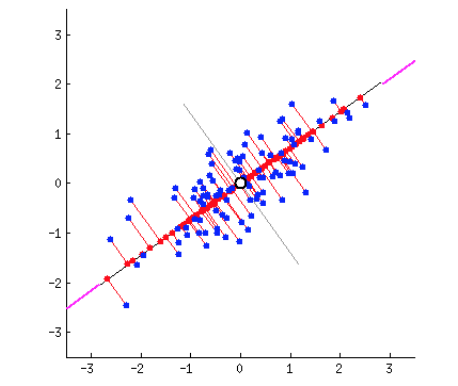
\includegraphics[scale=0.9]{notebooks/ML/img/pca_diagram.png}
    \caption{PCA Diagram}
\end{figure}
En problemas de clasificación o clustering, este enfoque puede ser útil para \textbf{visualizar etiquetas/clusters} en un gráfico de 2 o 3 dimensiones, o bien, puede ser utilizado para disminuir y condensar la información de un dataframe (\textit{feature extraction}). 

\begin{figure}[H]
\begin{subfigure}{.5\textwidth}
    \center
    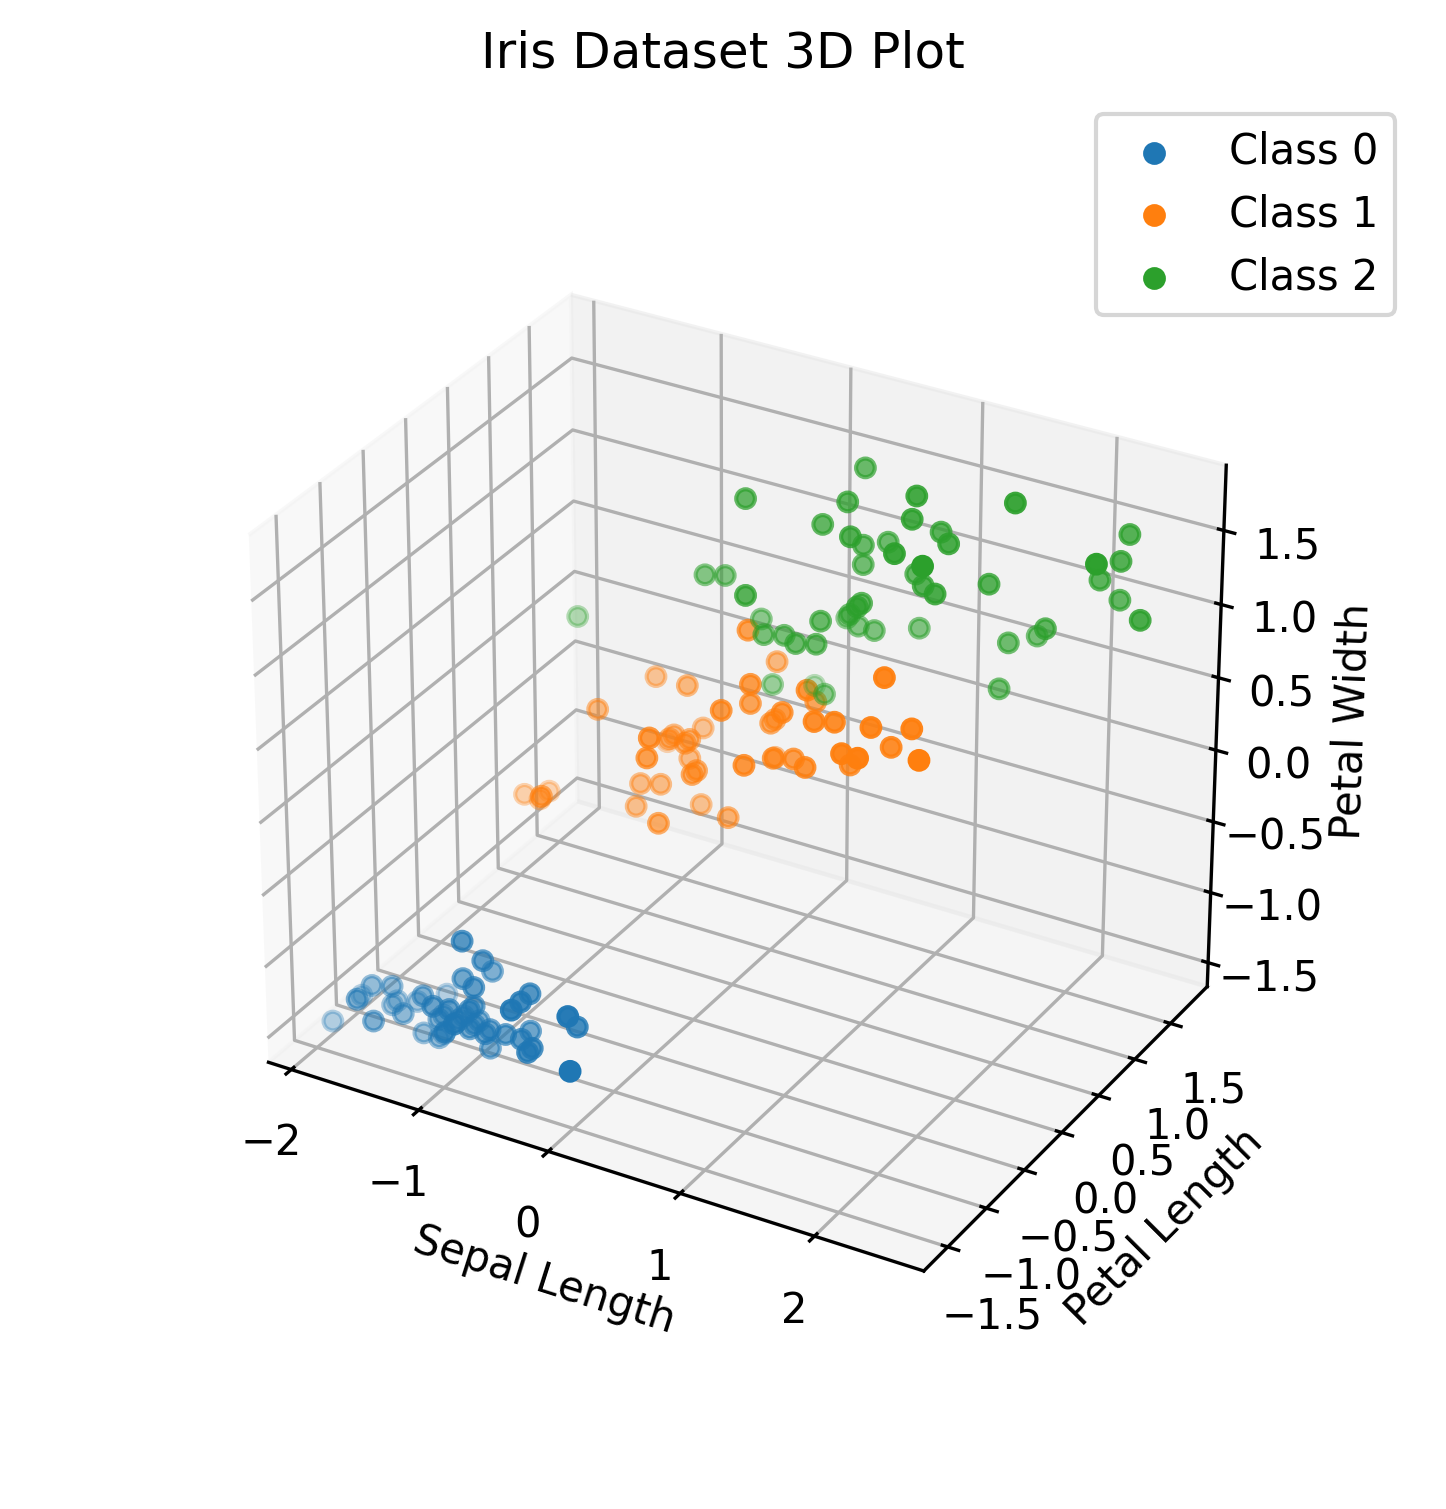
\includegraphics[scale=0.45]{notebooks/ML/img/3d_iris.png}
    \caption{3D Plot}
\end{subfigure}%
\begin{subfigure}{.5\textwidth}
    \center
    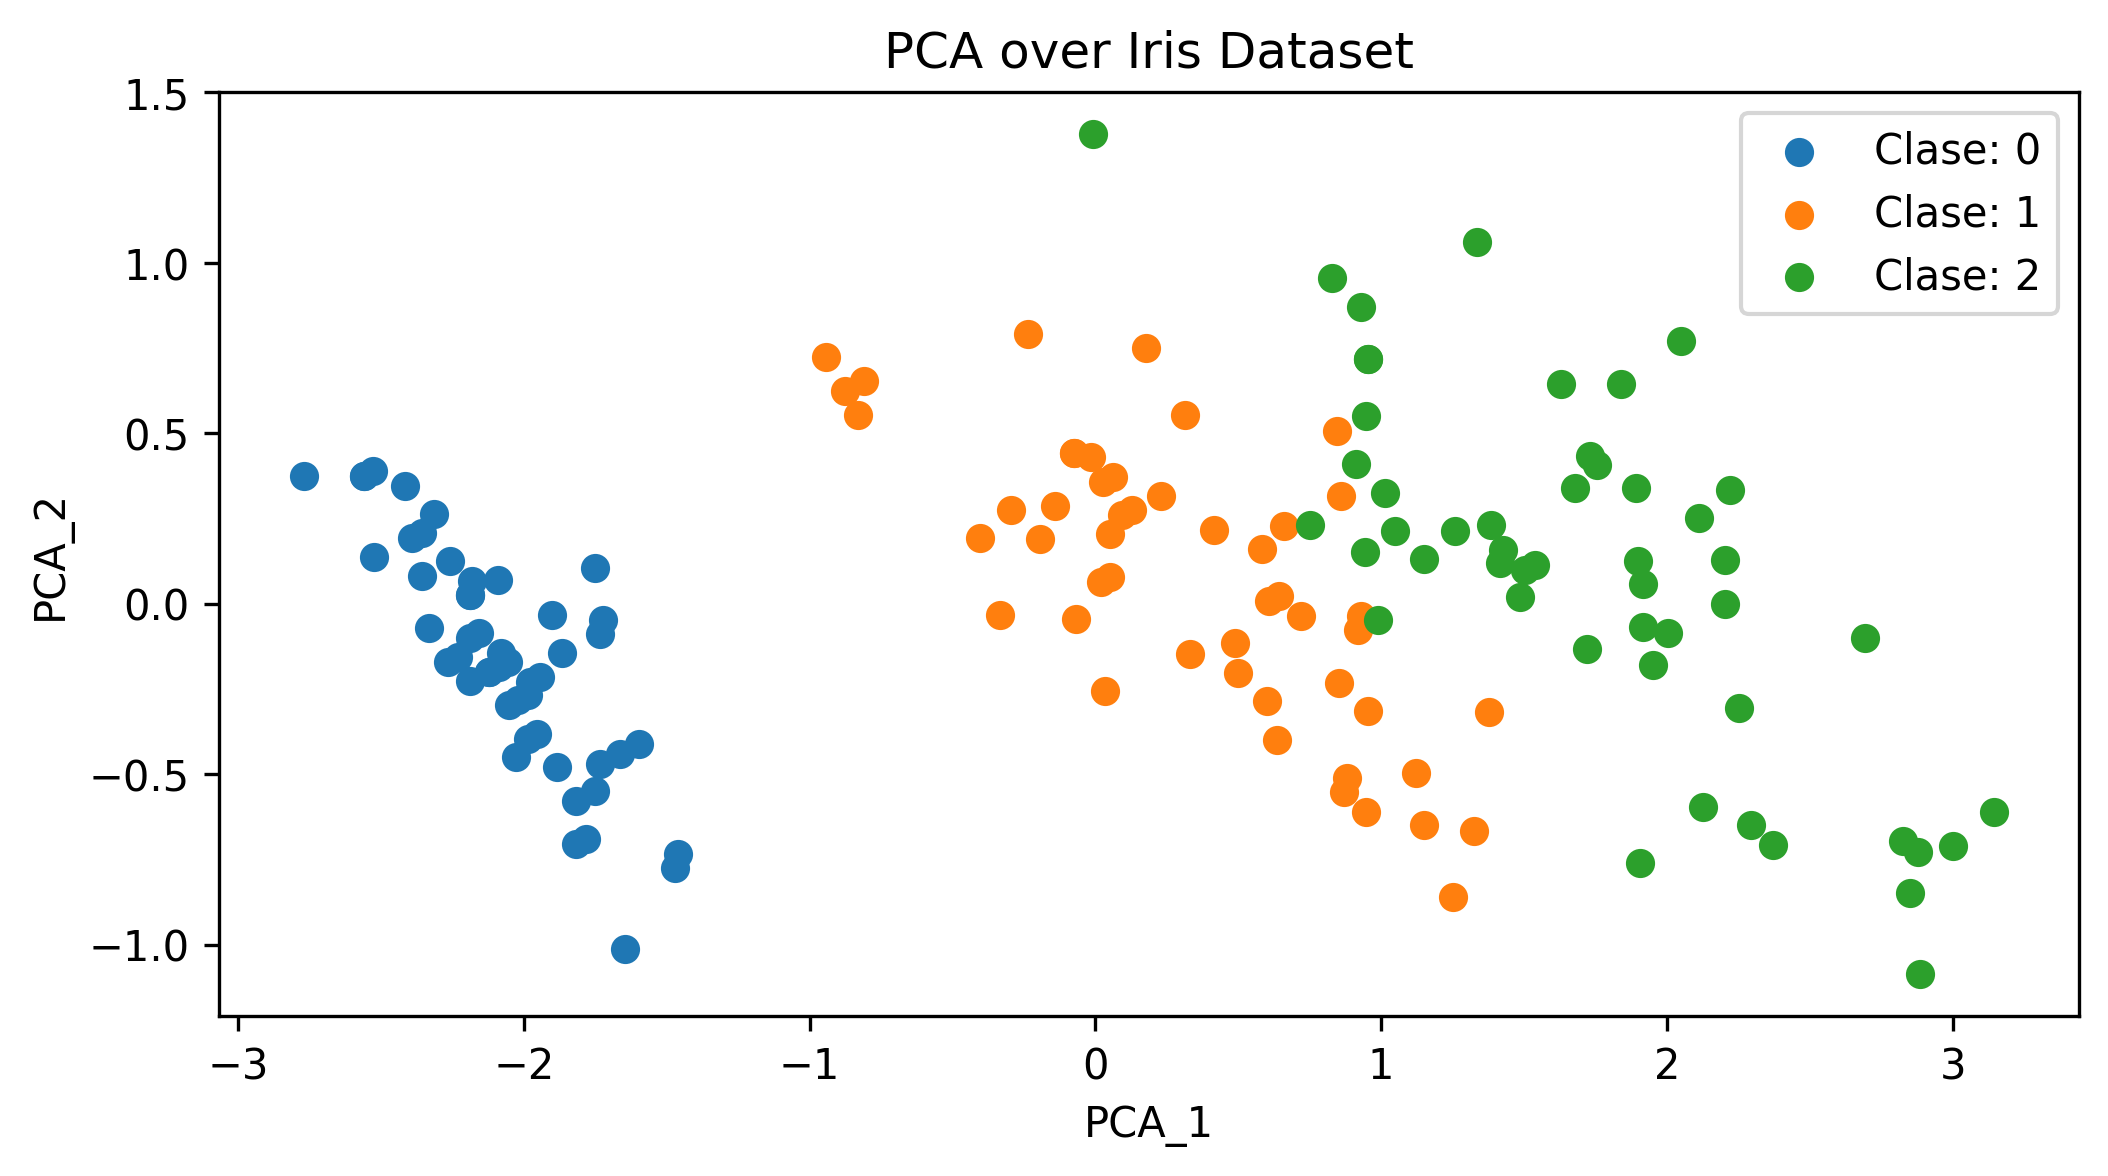
\includegraphics[scale=0.4]{notebooks/ML/img/pca_over_iris.png}
    \caption{2D PCA Plot}
\end{subfigure}
\caption{Iris Dataset}
\end{figure}

\section{t-Distributed Stochastic Neighbor Embedding (t-SNE)}

El algoritmo de t-SNE permite realizar una \textbf{reducción de dimensionalidad no lineal} de los datos para su simplificación y visualización. A diferencia del algoritmo de PCA, este no permite reducir la dimensión de nuevos datos pues \textbf{no aprende un mapping de espacios} en concreto, más bien, optimiza sobre los datos entregados. Por tanto, no es recomendable su uso para \textit{feature extraction}.

Para realizar esta reducción, en primer lugar se calcula la probabilidad $p_{ij}$ proporcional a la similitud entre los elementos $x_i$, $x_j$ según 

$$
p_{j|i} = \frac{\exp(-||x_i - x_j||^2 / 2\sigma_i^2)}{\sum_{k \neq i} \exp(-||x_i - x_k||^2 / 2\sigma_i^2)}
$$

Con $p_{i|i} = 0$. Notar que así $\sum_{j}p_{j|i} = 1$ para todo $i$, es decir, lo anterior define una distribución de probabilidad. Como la similitud entre $i$ y $j$ no es simétrica, definimos 
$$
p_{ij} = \frac{p_{i|j} + p_{j|i}}{2N}
$$

Ahora el objetivo es construir una distribución en una menor dimensionalidad, para este algoritmo, la distribución queda definida para los nuevos puntos $y_i$ según 

$$ 
q_{ij} = \frac{(1 + ||y_i - y_j||^2)^{-1}}{\sum_k \sum_{l \neq k} (1 + ||y_k - y_j||^2)^{-1}}
$$

Que resulta en una distribución $t-Student$ con 1 grado de libertad (esta forma de modelar la similitud es conveniente para alejar elementos poco similares). Para finalizar, los valores de $y_i$ son determinados minimizando la K-L divergencia mediante descenso de gradiente estocástico.

$$
KL(P || Q) = \sum_{i \neq j}p_{ij}\log \frac{p_{ij}}{q_{ij}}
$$

\begin{figure}[H]
    \center
    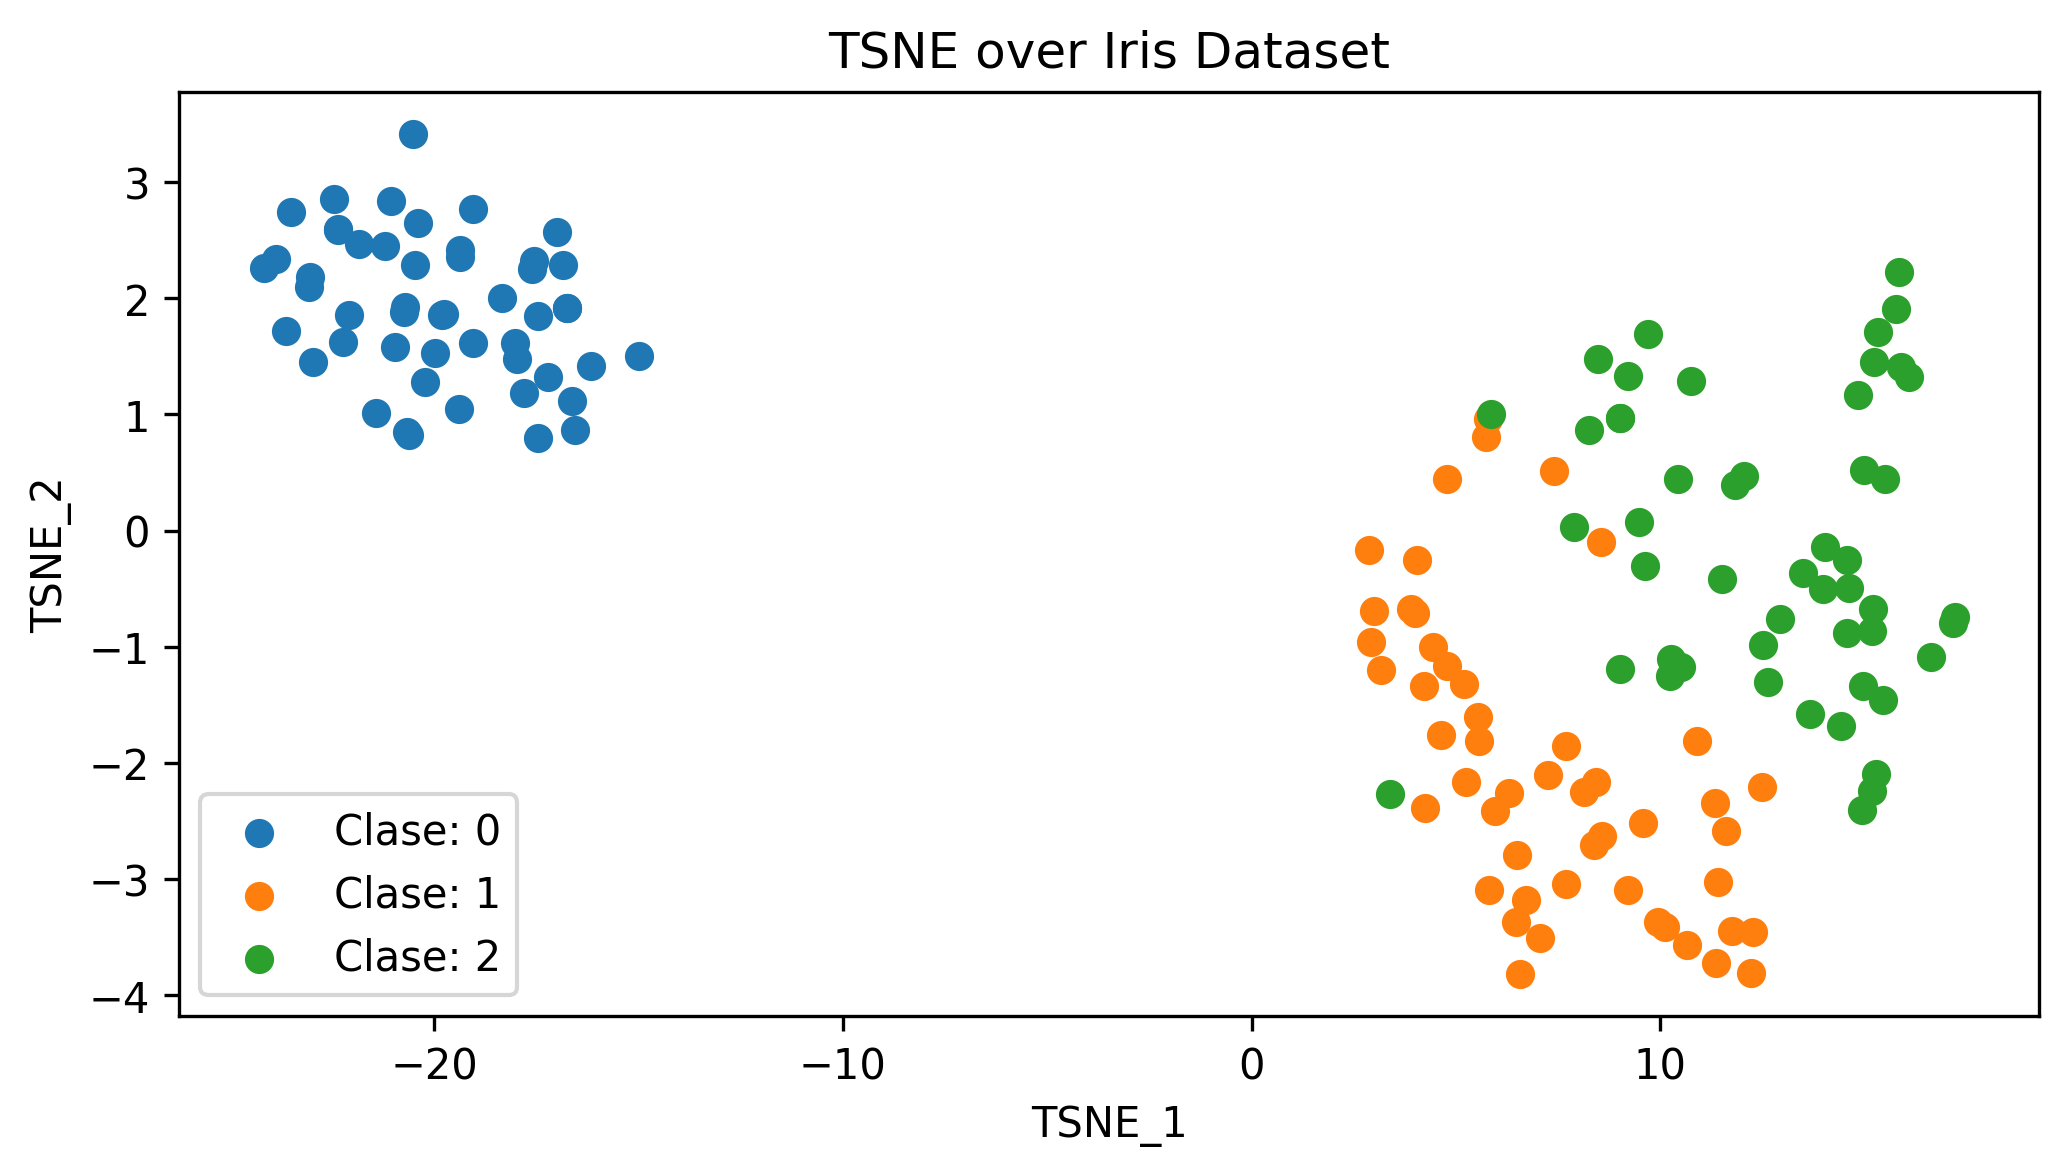
\includegraphics[scale=0.5]{notebooks/ML/img/tsne_over_iris.png}
    \caption{2D TSNE over Iris Dataset}
\end{figure}









\newpage

\chapter{Deep Learning}

\section{Gradient Descent}

\subsection{Algorithm}

El algoritmo de descenso de gradiente es un algoritmo de optimización sobre funciones de costo diferenciables. La ventaja de este algoritmo es que reduce enormemente la carga computacional en problemas de alta dimensión pero no asegura la convergencia global en funciones de costo no convexas. 

Consideremos una función de costo $J: \mathbb{R}^n \rightarrow \mathbb{R}$ diferenciable. En cada iteración del algoritmo, el parámetro $\theta$ se mueve en contra de la dirección del gradiente (problema de minimización) según
$$ 
\theta_{n+1} = \theta_n - \lambda \nabla J(\theta_n)
$$
Donde $\lambda > 0$ es un parámetro conocido como \textit{learning rate}. Notemos que, por expansión en serie de Taylor  centrada en $\theta_{n}$
$$ 
J(\theta_{n+1}) = J(\theta_{n}) + (\theta_{n+1} - \theta_{n})^{\top}\nabla J(\theta_n) + O(||\theta_{n+1} - \theta_{n}||^2)
$$
Aplicando la regla de descenso de gradiente 
$$ 
J(\theta_{n+1}) =  J(\theta_{n}) - \lambda \nabla J(\theta_n)^{\top}\nabla J(\theta_n) + O(||\lambda||^2) 
$$
Así 
$$
J(\theta_{n}) - J(\theta_{n+1}) = \underbrace{\lambda\nabla J(\theta_n)^{\top}\nabla J(\theta_n)}_{\geq 0} - O(||\lambda||^2)  \geq 0 
$$
Para $\lambda$ suficientemente pequeño. Así, $J(\theta_{n+1}) \leq J(\theta_n)$ y se demuestra la correctitud del algoritmo. 

\begin{figure}[H]
\begin{subfigure}{.5\textwidth}
    \center
    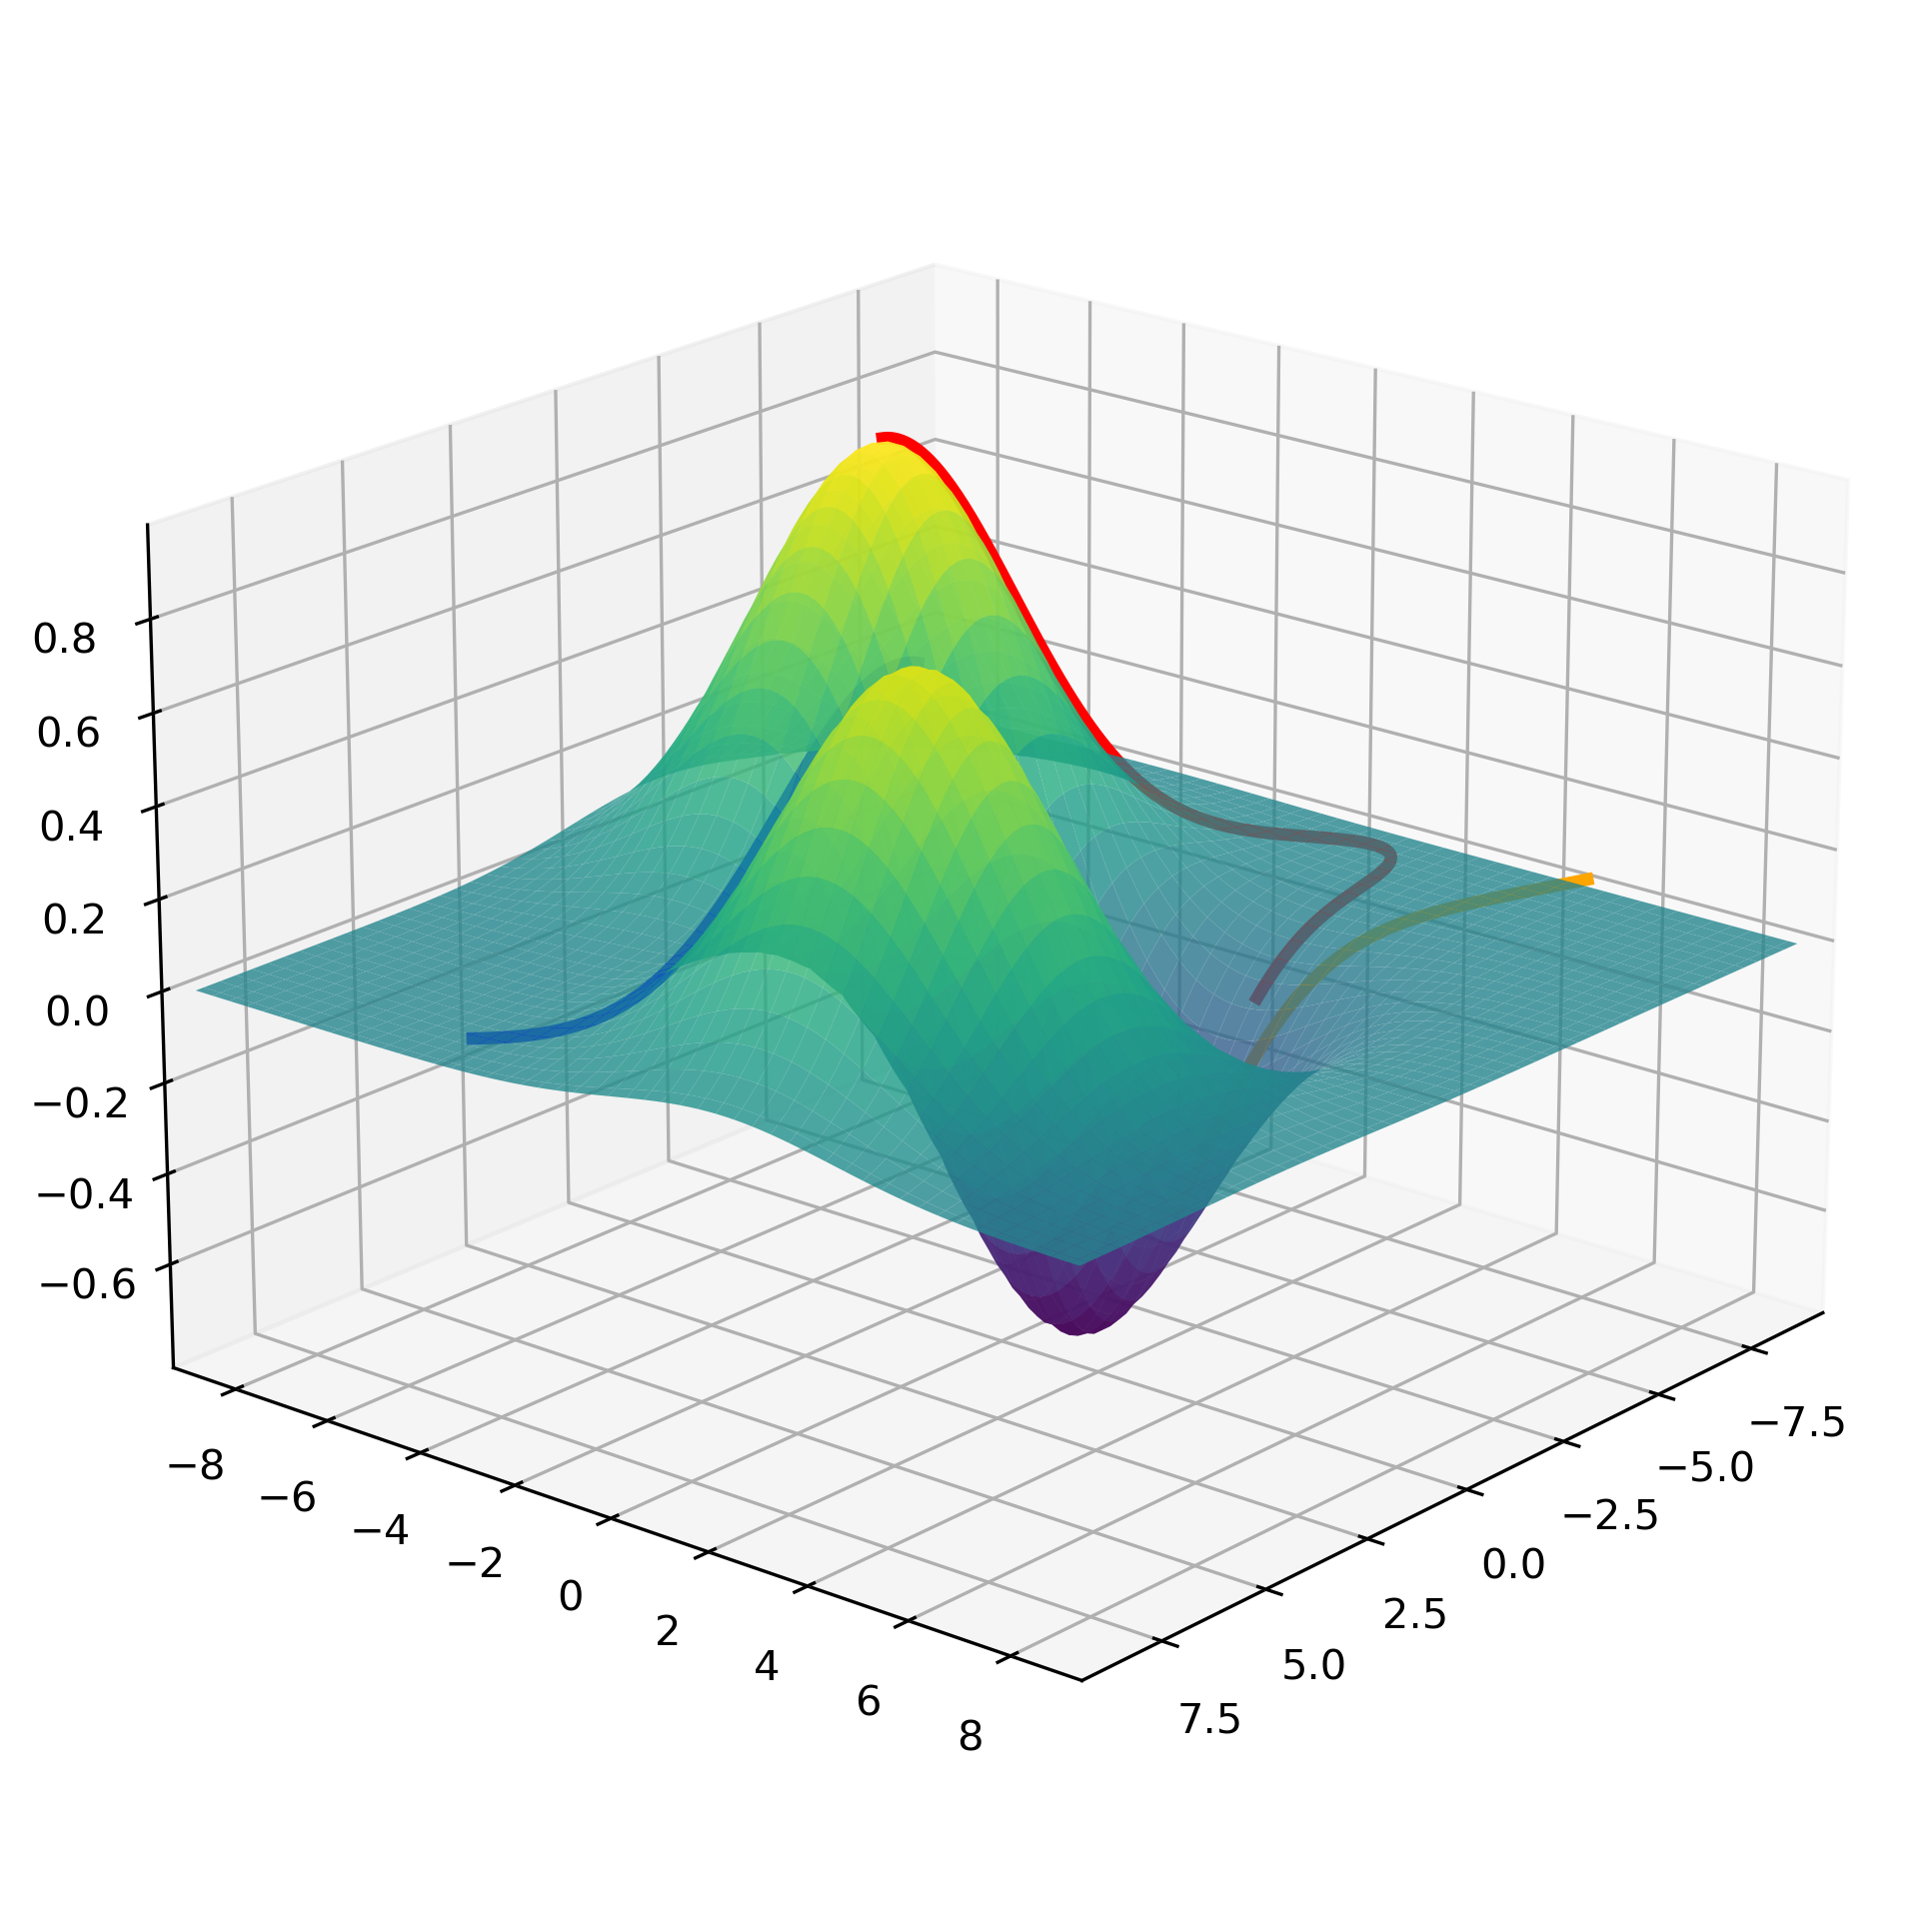
\includegraphics[scale=0.4]{notebooks/DL/img/3d_sgd.png}
    \caption{3D Plot}
\end{subfigure}%
\begin{subfigure}{.5\textwidth}
    \center
    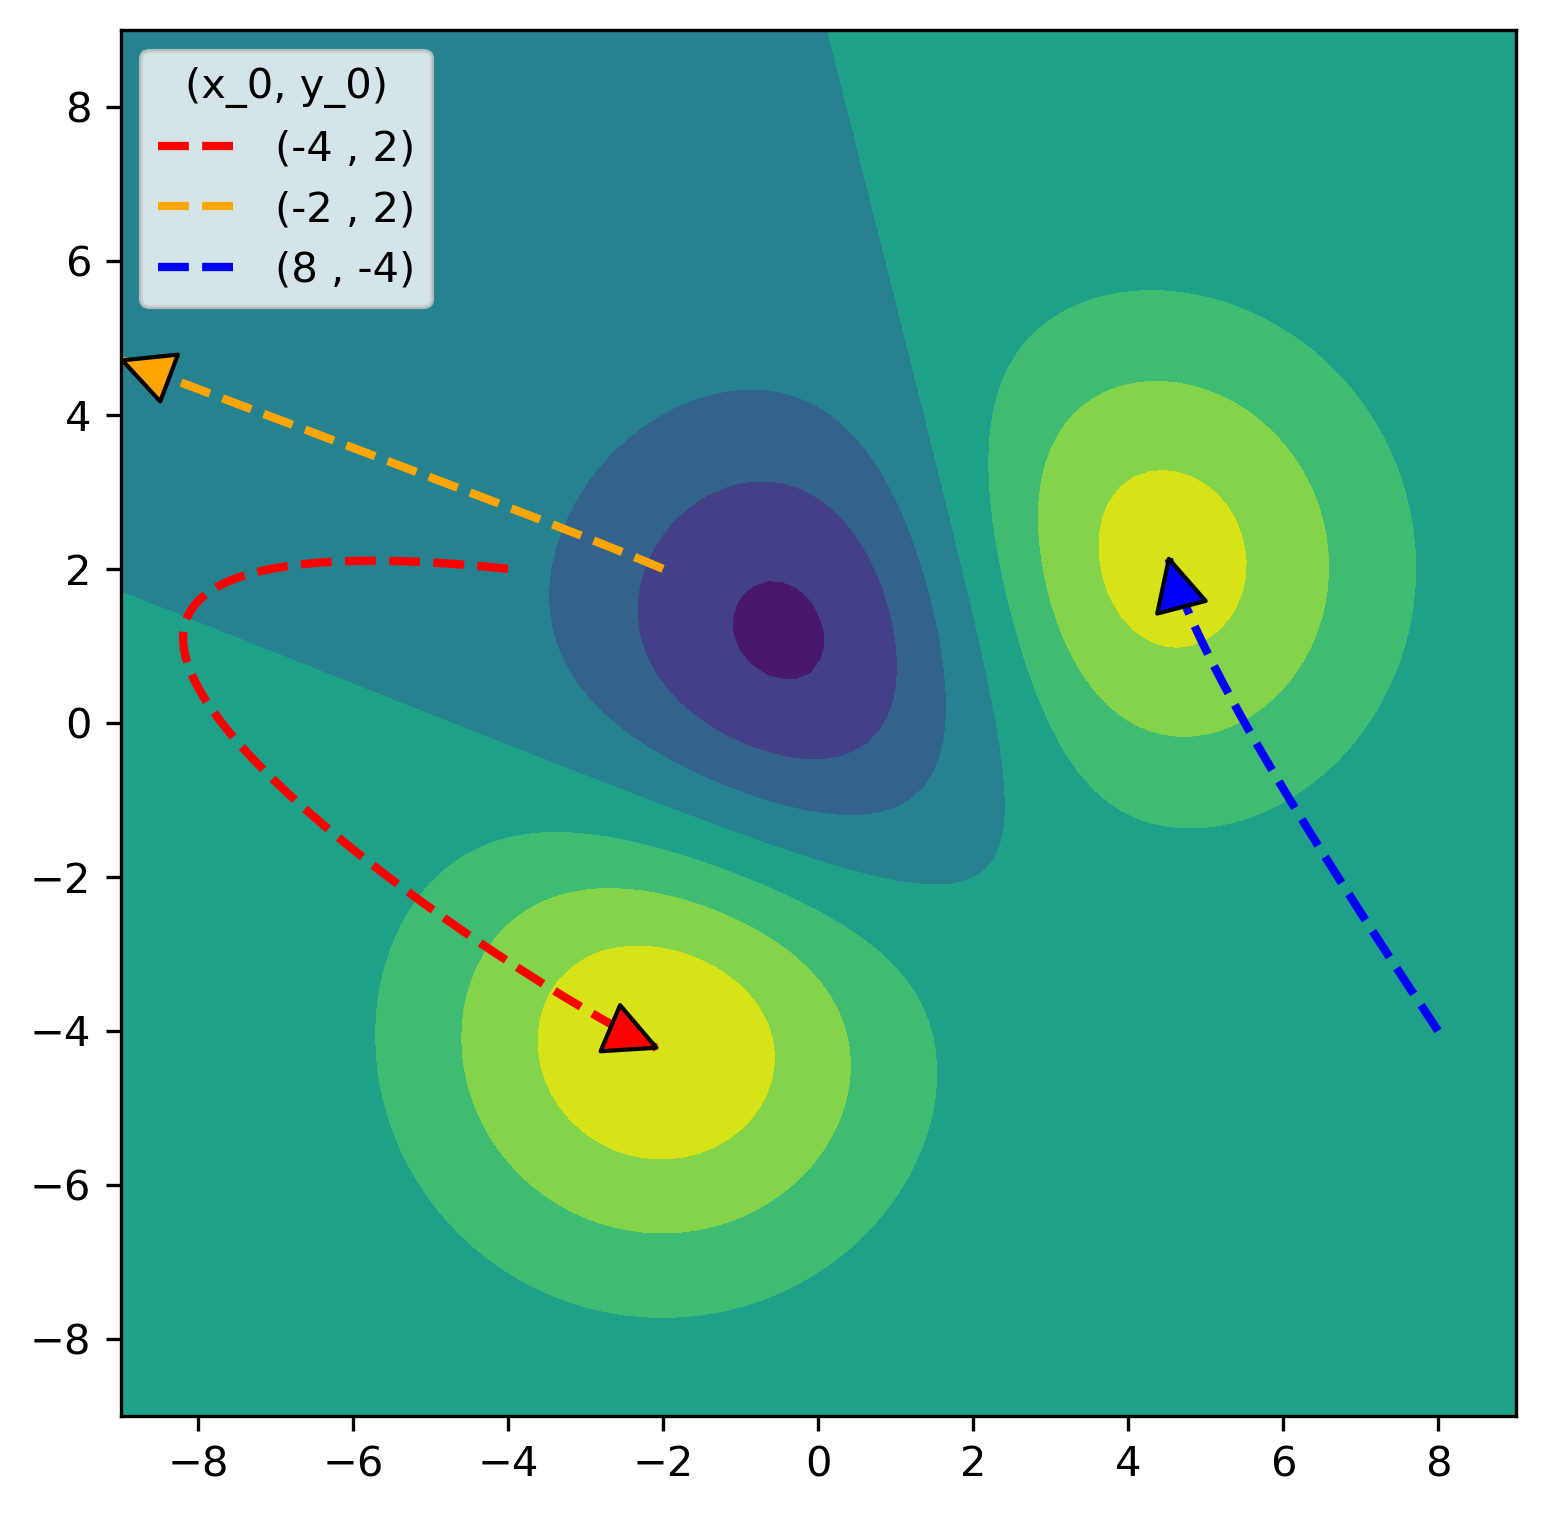
\includegraphics[scale=0.4]{notebooks/DL/img/contourf_sgd.png}
    \caption{Contour Plot}
\end{subfigure}
\caption{SGD Optimization for sum of Gaussian Distributions}
\end{figure}

\subsection{Stochastic Gradient Descent}

En problemas de Deep Learning, la función a minimizar $J$ dada una medida de desempeño $l(\hat{y},y) = l(f(x , \theta),y)$ se describe según 
$$ 
J^{*}(\theta) = \mathbb{E}_{(x,y) \sim p_{\text{data}}} l(f(x , \theta),y) .
$$
Que podemos aproximar por 
$$
J(\theta) = \mathbb{E}_{(x,y) \sim \hat{p}_{\text{data}}} l(f(x , \theta),y) = \frac{1}{k}\sum_{i=1}^{k}l(f(x_i , \theta),y_i)
$$
Con $k$ la cantidad de datos que consideremos en cada \textit{batch}. Entre menor sea el tamaño del batch, mayor será el ruido en la convergencia pero menor el costo computacional.

\begin{figure}[H]
    \center
    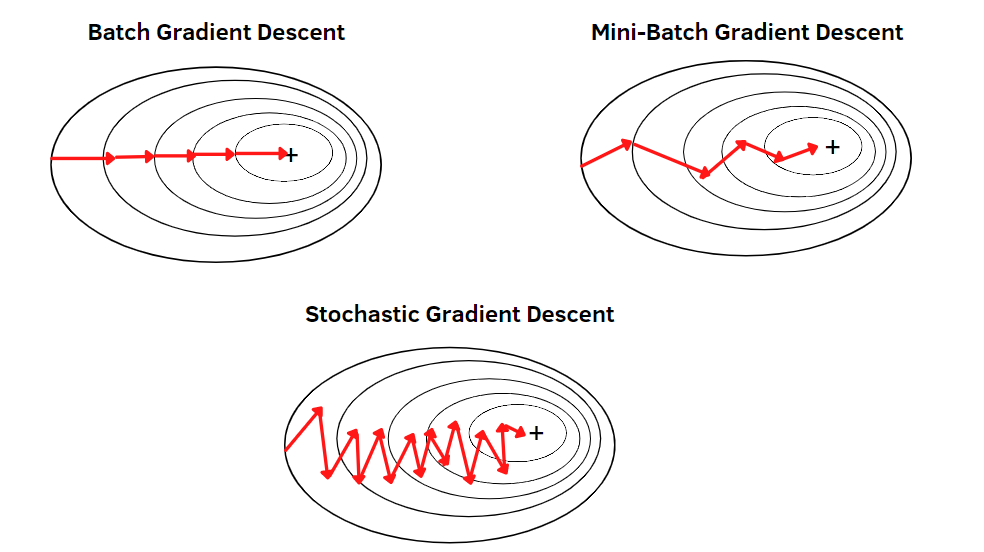
\includegraphics[scale=0.25]{notebooks/DL/img/sgd_diagram.png}
    \caption{SGD Diagram}
\end{figure}


\newpage

\section{Statistics}

\subsection{Causal Inference}

La inferencia causal es el proceso de determinar el \textbf{efecto independiente de una variable} en un sistema más complejo. En general, este proceso es necesario cuando buscamos obtener conclusiones de datos pasados y en los que no es posible realizar un \textit{A/B testing}.

Existen 3 desafíos al realizar este proceso: 
\begin{itemize}
    \item \textbf{Cofounders}: Son aquellas variables que tienen un impacto en el \textit{outcome} y que incluso podrían tener un impacto en otras variables. 
    \item \textbf{Selection Bias}: Selección no representativa del grupo de control y tratamiento.
    \item \textbf{Counterfactuals}: Imputar valores en el grupo de control y tratamiento en base a \textit{Machine Learning} o algoritmos de \textit{Matching}. 
\end{itemize}

\begin{figure}[H]
    \center
    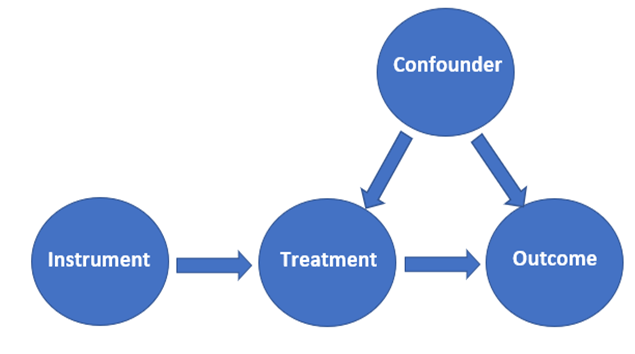
\includegraphics[scale=0.3]{notebooks/STATS/img/causal_inference_diagram.png}
    \caption{Casual Inference - DAG Diagram}
\end{figure}

Para resolver este problema, es necesario tomar algunos supuestos: 
\begin{enumerate}
    \item \textbf{Causal Markov Condition}: La influencia de las variables y el \textit{outcome} puede ser representado a través de un \textbf{Grafo Acíclico Dirigido (DAG)} en el que se asume la \textbf{condición de Markov}, es decir si $Y \rightarrow S \rightarrow C$, podemos asumir que $C \indep Y | S$
    \item \textbf{SUTVA}: (Stable Unit Treatment Value Assumption) El grupo de control y tratamiento \textbf{no tiene influencia el uno con el otro}. 
    \item \textbf{Ignorability}: Se excluye el ruido proveniente de cualquier otra fuente. 
\end{enumerate}

Consideremos el siguiente ejemplo en el que buscamos determinar si el efecto de un tratamiento tiene un impacto en una variable \textit{target}. 

\begin{figure}[H]
    \center
    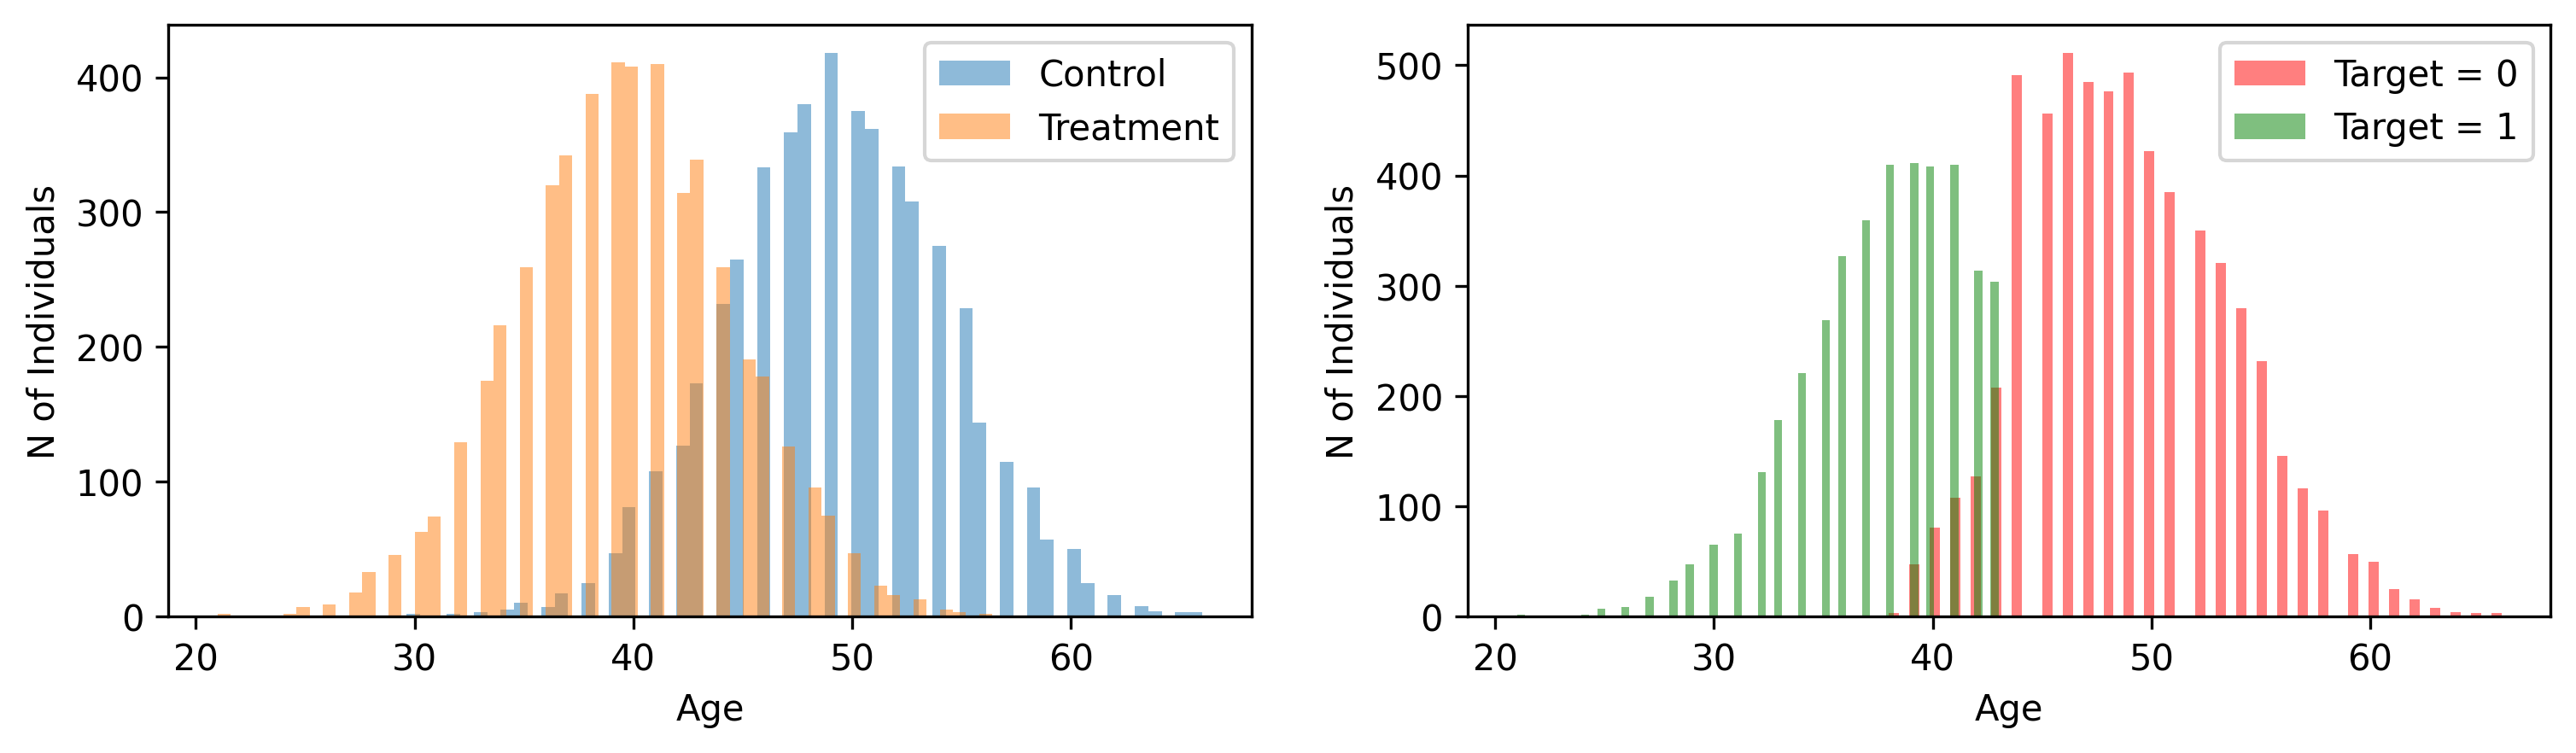
\includegraphics[scale=0.5]{notebooks/STATS/img/causal_inference_age_distribution.png}
    \caption{Casual Inference - Distribution Example}
\end{figure}

Vemos que existe un \textit{selection bias} pues el grupo de tratamiento y control tienen distribuciones de edad distintas. Existen múltiples enfoques para resolver este problema. 

\subsubsection{Matching Imputation}

Es posible utilizar un algoritmo de \textit{Matching} como \textit{NearestNeighbors} para imputar el posible \textit{outcome} que hubiese tenido un individuo al recibir o no el tratamiento. En nuestro ejemplo, para cada edad de los individuos del grupo de control, buscaríamos al sujeto con la edad más cercana en el grupo de tratamiento e imputaríamos su respuesta al tratamiento y viceversa. 

La efectividad del tratamiento se puede medir a través del promedio de los \textit{outcome} cuando reciben y cuando no reciben el tratamiento. 

\subsubsection{Meta Learners}

Este enfoque plantea utilizar algoritmos de \textit{Machine Learning} para determinar el efecto del tratamiento en el \textit{outcome} del experimento. Sea $y_i$ el \textit{target}, $w$ si recibió el tratamiento y $X_i$ el conjunto de variables del modelo, definimos ITE (\textit{Individual Treatment Effect}) según 
$$
\text{ITE} = \left [ p(y_i = 1 | w_i = 1, X_i) - p(y_i = 1 | w_i = 0, X_i) \right ]
$$

\begin{itemize}
    \item \textbf{S - Model} Este algoritmo es el más simple de todos pues agrega la variable \textit{treatment} como input de un único modelo. El valor de ITE es calculado para cada individuo variando el valor del tratamiento. 
    \item \textbf{T - Model} Este algoritmo entrena 2 clasificadores, uno encargado del grupo de control y otro para el grupo de tratamiento. El valor de ITE es calculado como la resta del \textit{output} de ambos modelos. 

    Hay que tener en consideración que este modelo requiere una \textbf{calibración} para asegurar que el \textit{output} de los modelos sean probabilidades.
    \item \textbf{X - Model}: SOON 
\end{itemize}


\begin{figure}[H]
    \center
    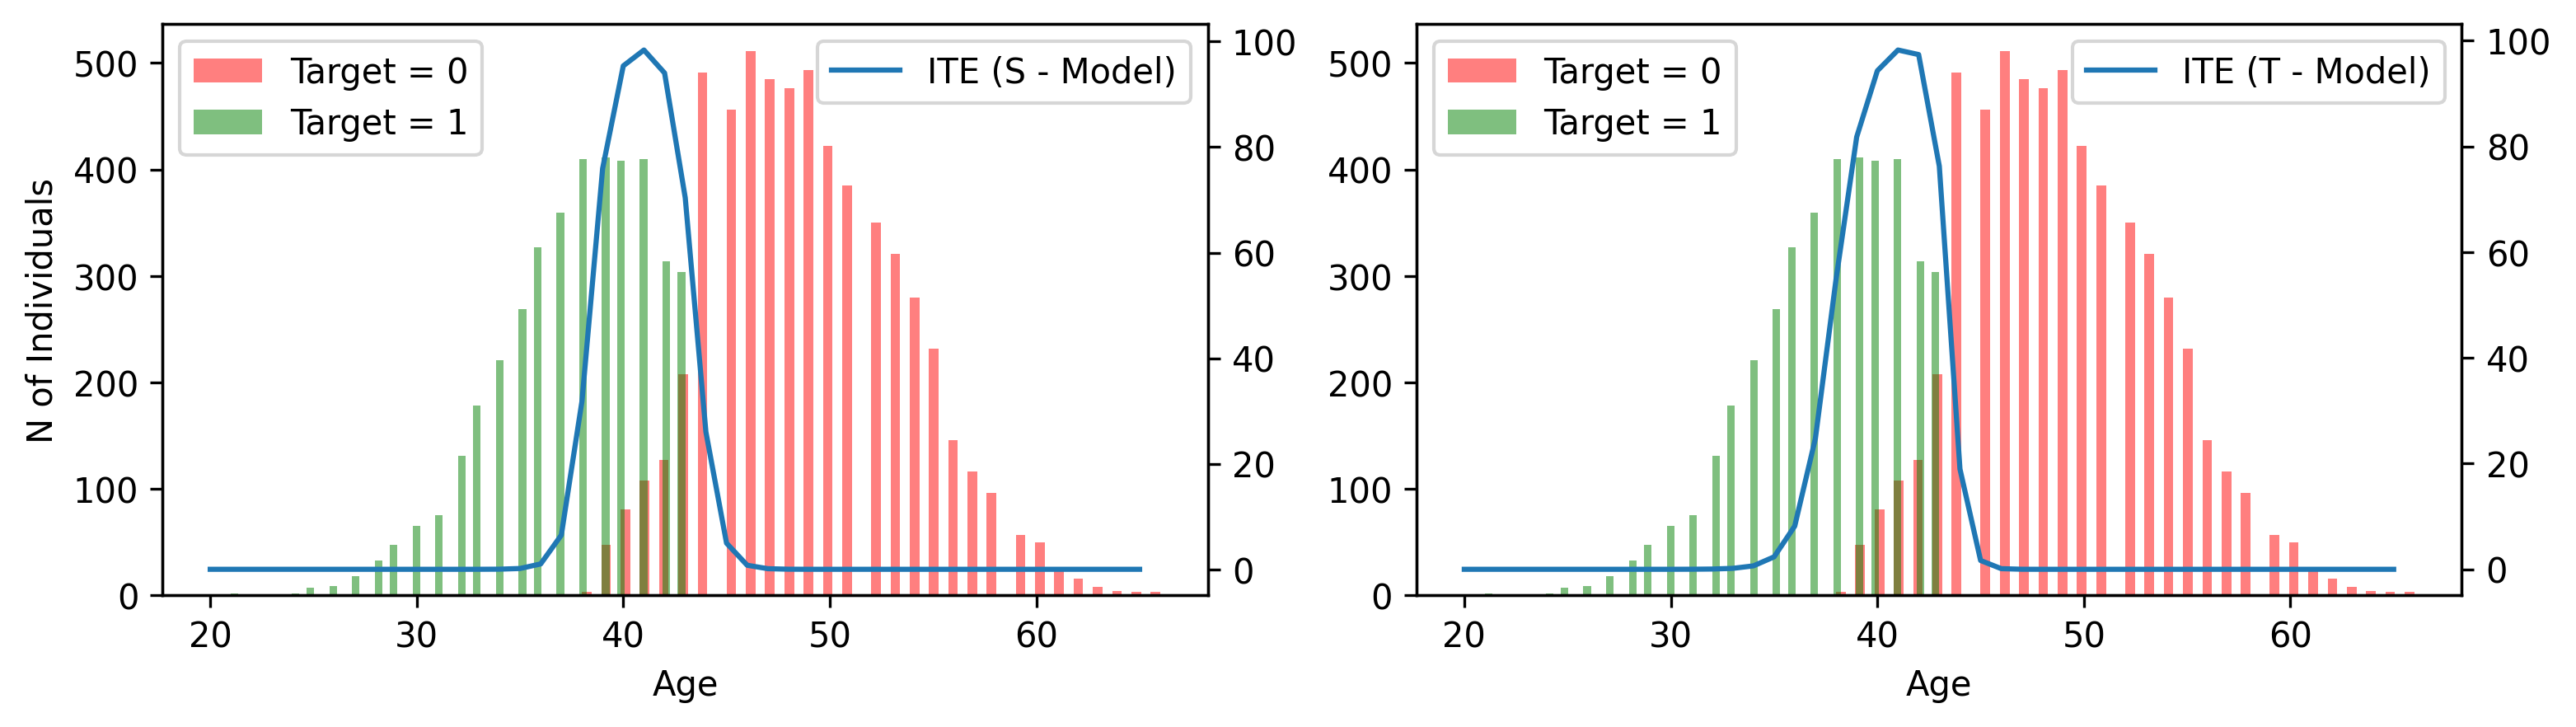
\includegraphics[scale=0.5]{notebooks/STATS/img/causal_inference_meta_learners.png}
    \caption{Meta Learners}
\end{figure}

Vemos así que el impacto del tratamiento aislando el efecto de la edad, ocurre según ITE entre los 35 y 45 años. 






\newpage

\section{Others}

\subsection{Performance Metrics} 

\subsection{Bias vs Variance}

El dilema de \textit{Bias vs Variance} describe la relación entre la complejidad del modelo, la precisión de las predicciones y cómo éste se comporta al predecir datos nunca antes vistos. El error estimado de una predicción viene dado en términos generales por 
$$
\text{Expected Error} = (\text{Bias})^2 + \text{Variance} + \text{Irreductible Error}
$$
Así, un modelo que crece en complejidad reducirá su bias pero aumentará su varianza (extremo: overfitting) y a la vez, reducir la complejidad permitirá generalizar mejor reduciendo la varianza pero aumentando el bias (extremo: underfitting). 

\begin{figure}[H]
    \center
    \includegraphics[scale=0.3]{notebooks/Others/img/bias_vs_variance.png}
    \caption{Bias vs Variance Diagram}
\end{figure}

\subsection{Oversampling and Undersampling}

\subsection{Random Noise Feature Importance}

\subsection{SHAP Values}
\label{subsec:shap_values}

El SHAP values (\textit{SHapley Additive exPlanations}) es un algoritmo modelo-agnóstico basado en teoría de juegos que permite \textbf{interpretar las predicciones}, la importancia de las variables y su impacto.

\begin{figure}[H]
    \center
    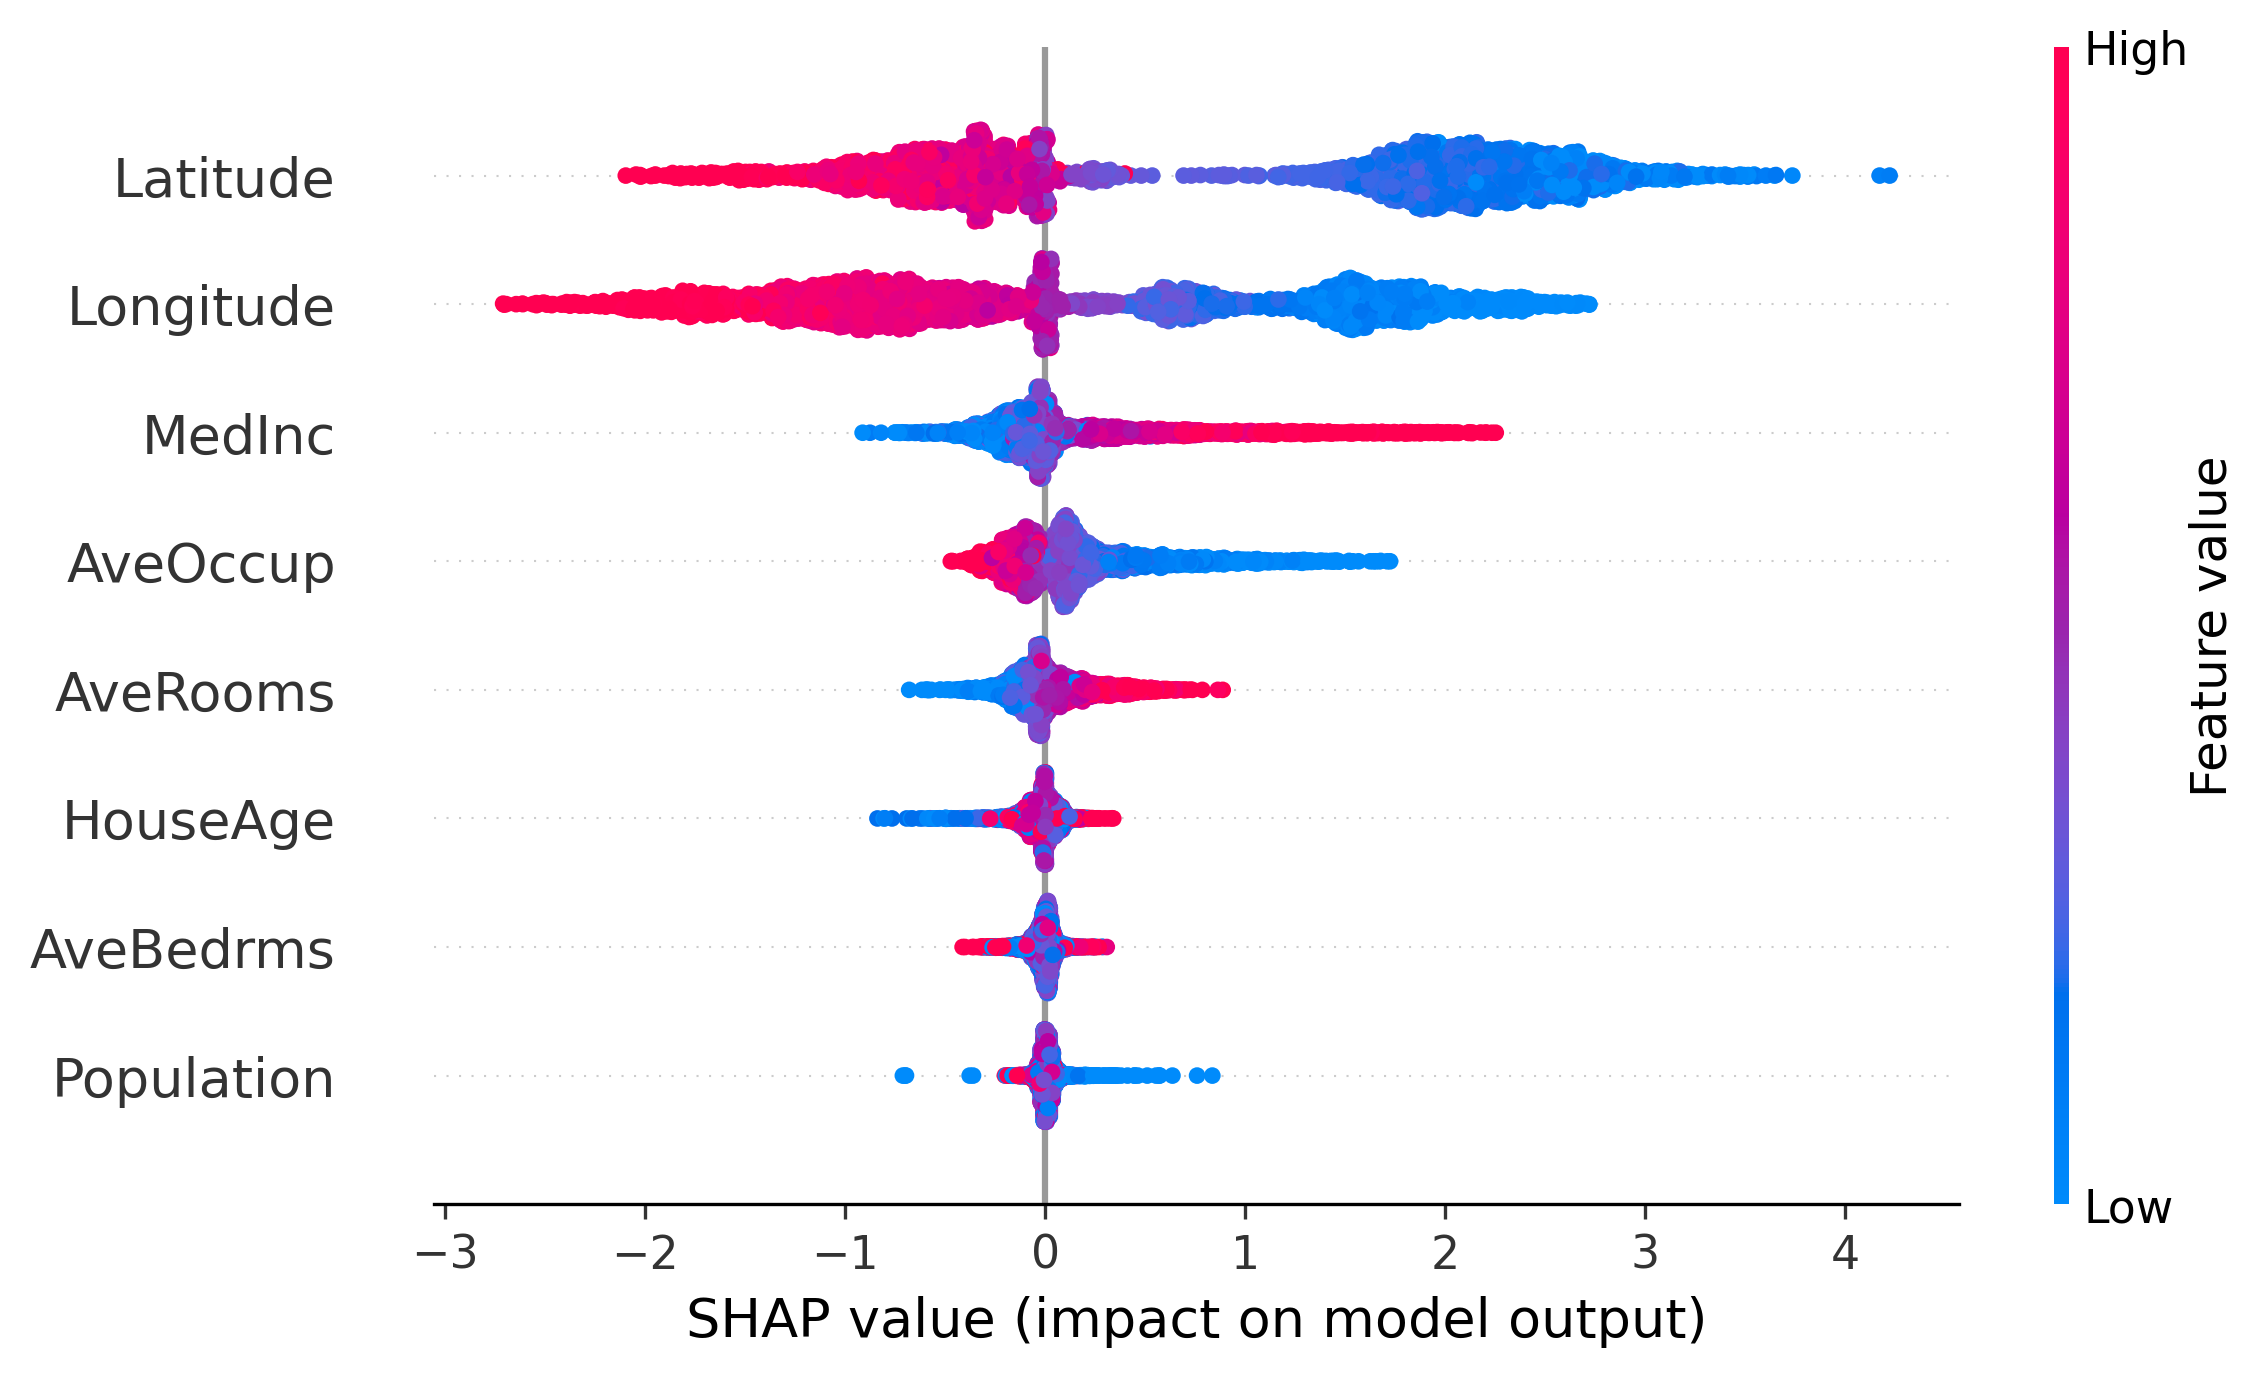
\includegraphics[scale=0.55]{notebooks/Others/img/shap_values_example.png}
    \caption{SHAP Values Example}
\end{figure}

\subsection{Outlier Detection}

La detección de outliers es la práctica de encontrar \textbf{datos anómalos} o fuera de distribución en un dataset. Es de suma importancia para la construcción de modelos de fraude o para mejorar el performance de modelos sensibles a outliers.

\begin{figure}[H]
    \center
    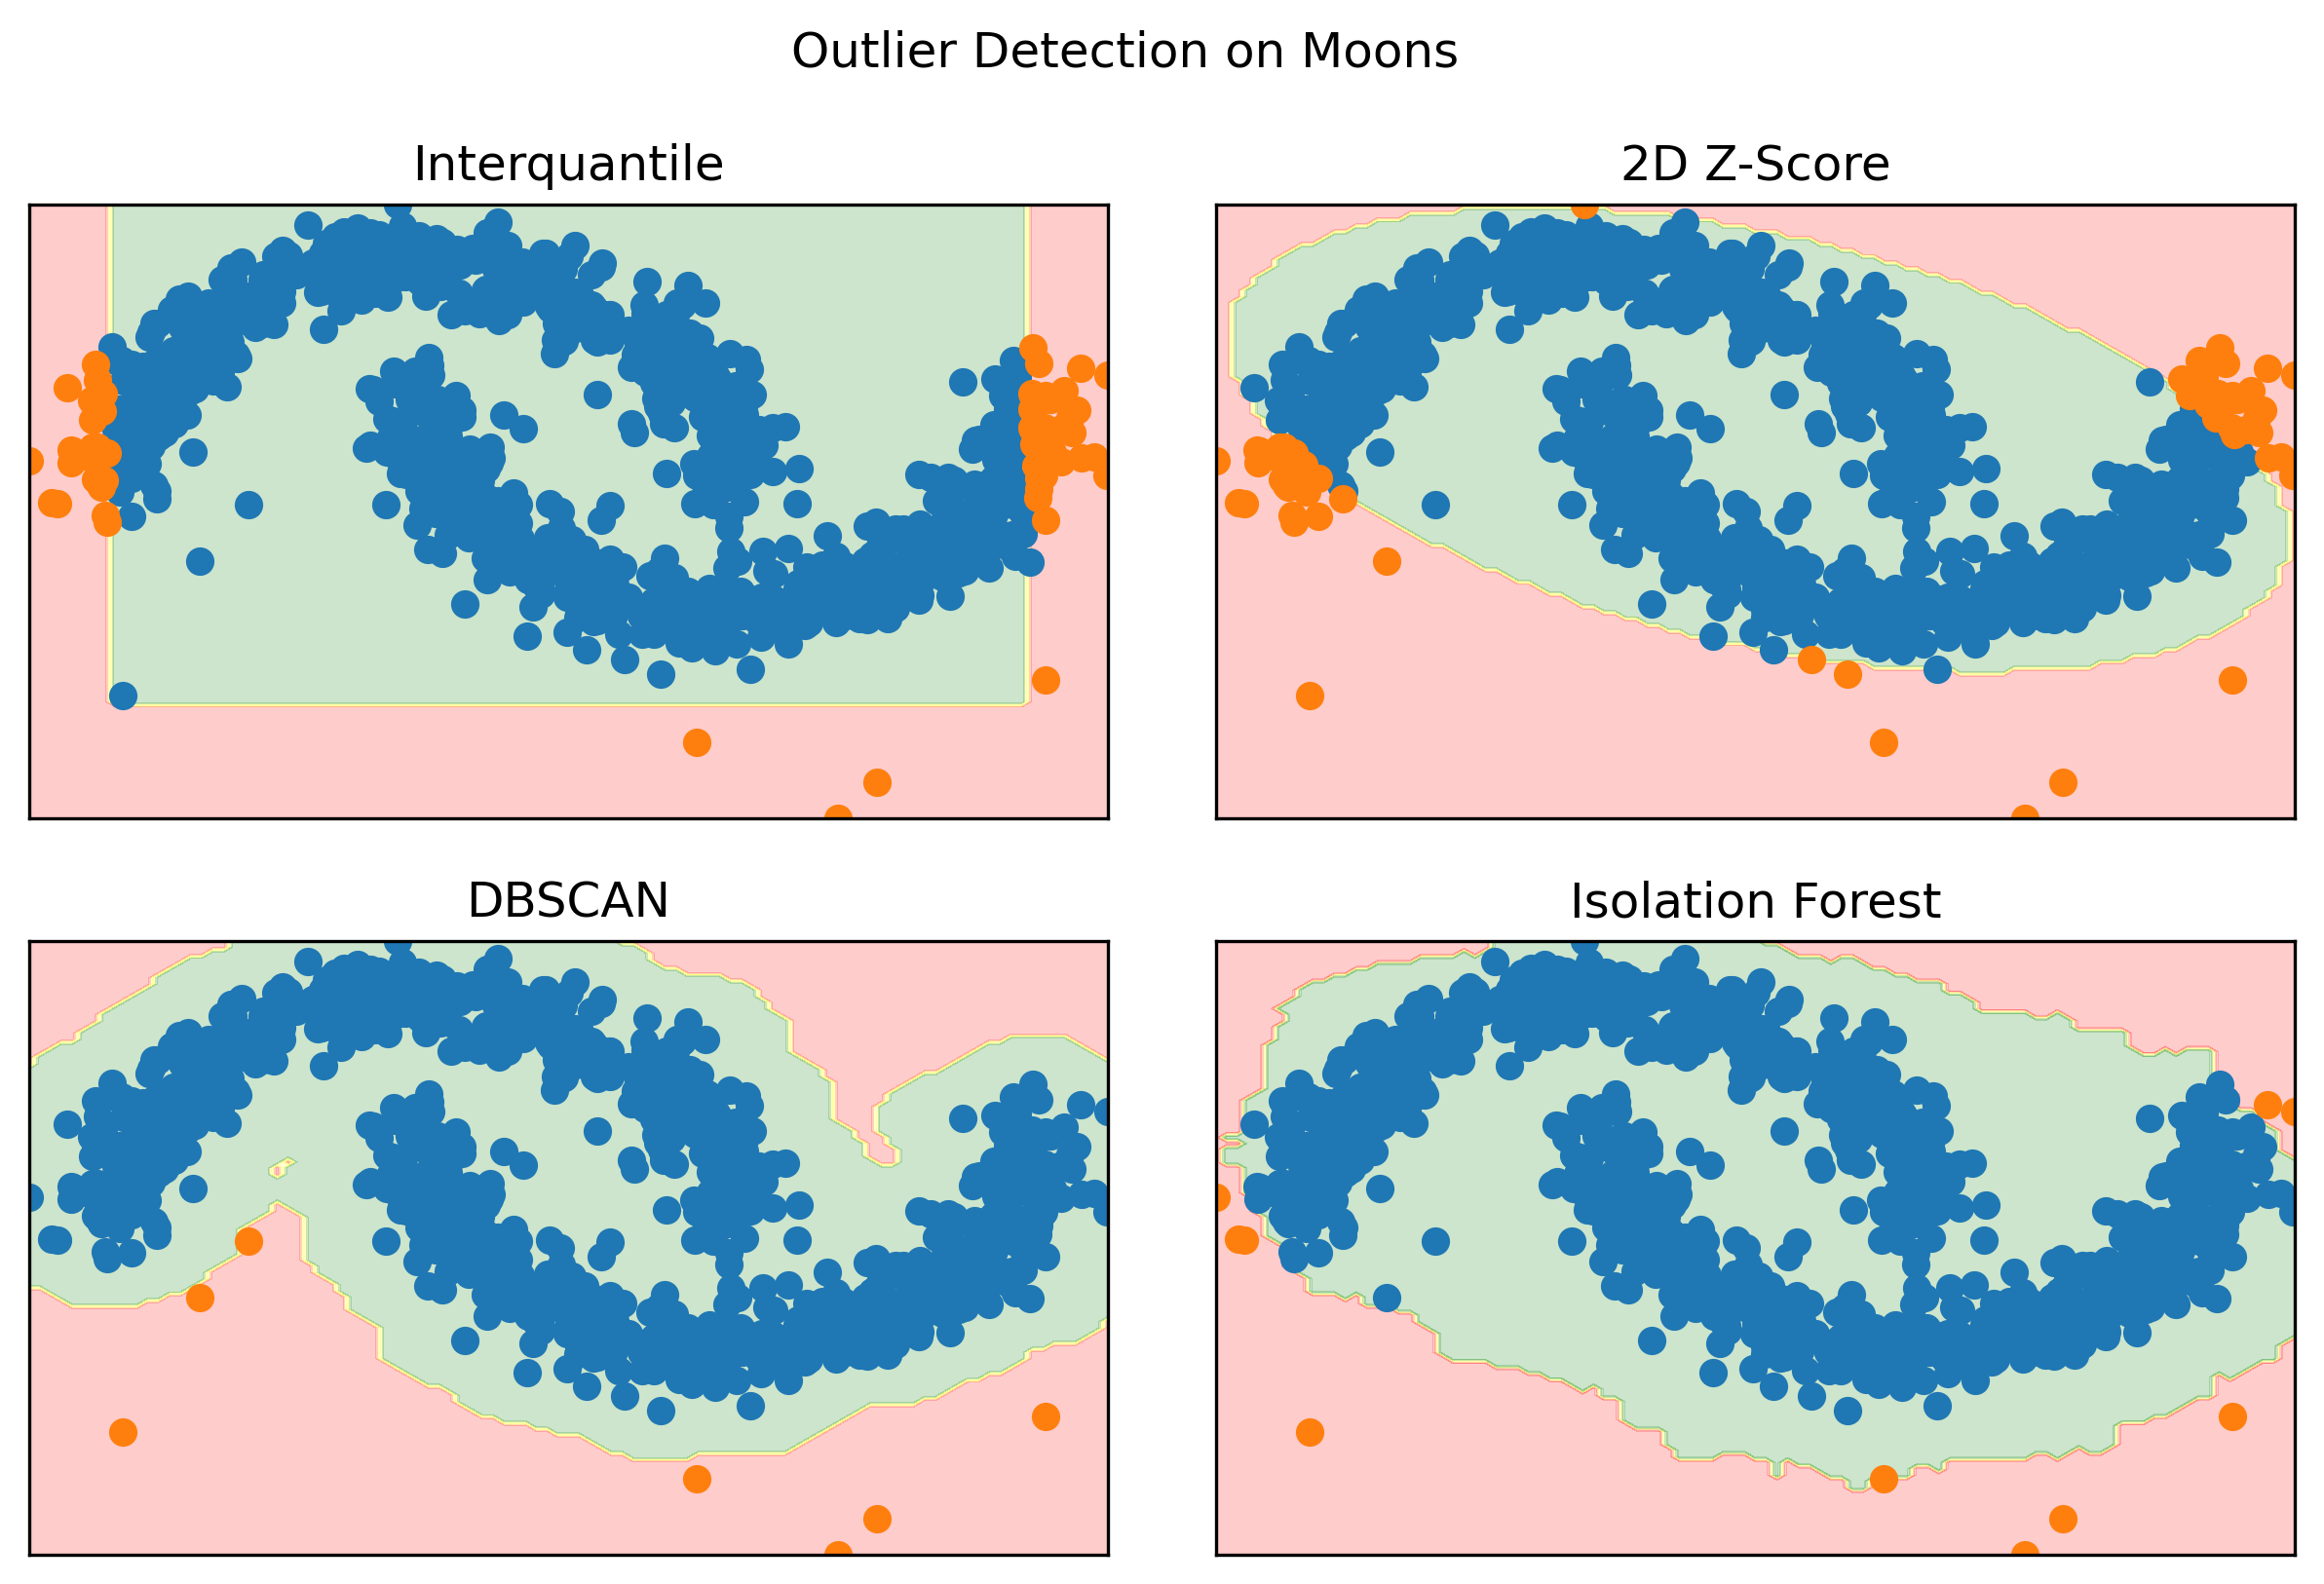
\includegraphics[scale=0.55]{notebooks/Others/img/outlier_detection.png}
    \caption{Outiler Detection Contour Plot}
\end{figure}

\subsubsection{Interquantile Range}

Definimos el \textit{Interquantile Range} IC como la diferencia entre el percentil 75 y el percentil 25. Es decir, 
$$ 
IC = Q_3 - Q_1
$$
En este caso, los outliers serán aquellos datos $x_i$ tal que 
$x_i \geq Q3 + I_{\text{range}}IC$ o bien $x_i \leq Q1 - I_{\text{range}}IC$
donde $ I_{\text{range}}$ permite controlar el porcentaje de outliers que se espera encontrar. (Equivalencia en distribución normal $I_{\text{range}} = 1.5 \approx Z_{\text{value}} = 2.69$).

Notar que en esta metodología no se asume normalidad en la distribución de los datos. 

\subsubsection{Z - Score}

Cuando los datos siguen una distribución normal, se pueden considerar como outliers aquellos datos $x_i$ que cumplen 
$$\left | \frac{x_i - \mu}{\sigma}\right | \geq Z_{\text{value}}$$

Para los casos con más de una feature (multidimensional), se puede extender esta definición utilizando la \textbf{distancia de Mahalanobis} definida como 
$$
D = \sqrt{(x_i - \mu_i)^{\top}\Sigma^{-1}(x_i - \mu_i)}
$$
Donde $\Sigma$ es la matriz de covarianza y $\mu_i$ el vector de media. 

\subsubsection{DBSCAN}

Los datos que no cumplan el mínimo de vecinos a distancia menor de $\epsilon$ son considerados por DBSCAN como outliers.

\subsubsection{Isolation Forest}

El algoritmo de \textit{Isolation Forest} selecciona de manera aleatoria una feature y un corte aleatorio entre el mínimo y el máximo valor presente en esa feature. Esto es repetido múltiples veces hasta aislar cada uno de los puntos.

Este algoritmo iterativo, puede ser representado en el siguiente diagrama:

\begin{figure}[H]
    \center
    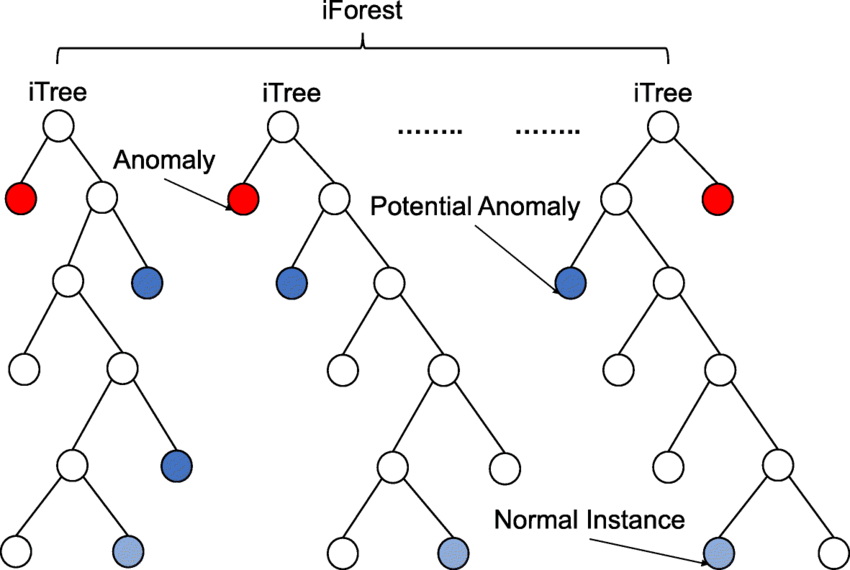
\includegraphics[scale=0.3]{notebooks/Others/img/isolation_forest_diagram.png}
    \caption{Isolation Forest Diagram}
\end{figure}

Los puntos que en promedio, requieren \textbf{menos divisiones para ser aislados}, son los que el algoritmo considera como potenciales datos anómalos (outliers).

\subsection{Cross-Validation Techniques}

El \textit{Cross-Validation} es un método que permite evaluar el rendimiento de un modelo de \textit{Machine Learning} y que busca eliminar el sesgo de la elección del conjunto de entrenamiento y testeo. Es ampliamente utilizado para la búsqueda de los mejores hiper-parámetros de un modelo. 


\begin{enumerate}
    \item \textbf{KFold}: Esta técnica consiste en dividir el conjunto de entrenamiento en $k$ partes. En cada iteración, se selecciona una de las particiones para testing y el resto para training. El score será el promedio de los scores obtenidos. Existe una variación llamada \textbf{StratifiedKFold} en la cual se asegura además que el target tenga la misma distribución en cada partición.
    \item \textbf{ShuffleSplit}: Esta técnica selecciona la partición de entrenamiento y testing de manera aleatoria. No asegura que las particiones sean las mismas en cada iteración. 
    \item \textbf{LeavePOut}: Esta técnica deja $p$ datos para el conjunto de testeo y entrena con todo el resto. Este proceso se realiza con todas las combinaciones posibles lo que asegura una estimación con menor bias aunque es extremadamente ineficiente. 
\end{enumerate}

\subsubsection{Time Series Cross Validation}

En el caso de series de tiempo, es importante notar que al momento de realizar \textit{Cross-Validation} para problemas de Forecast, es importante \textbf{no entrenar con datos posteriores al testing} pues en la práctica, no se tendría acceso a estos.

\begin{figure}[H]
    \center
    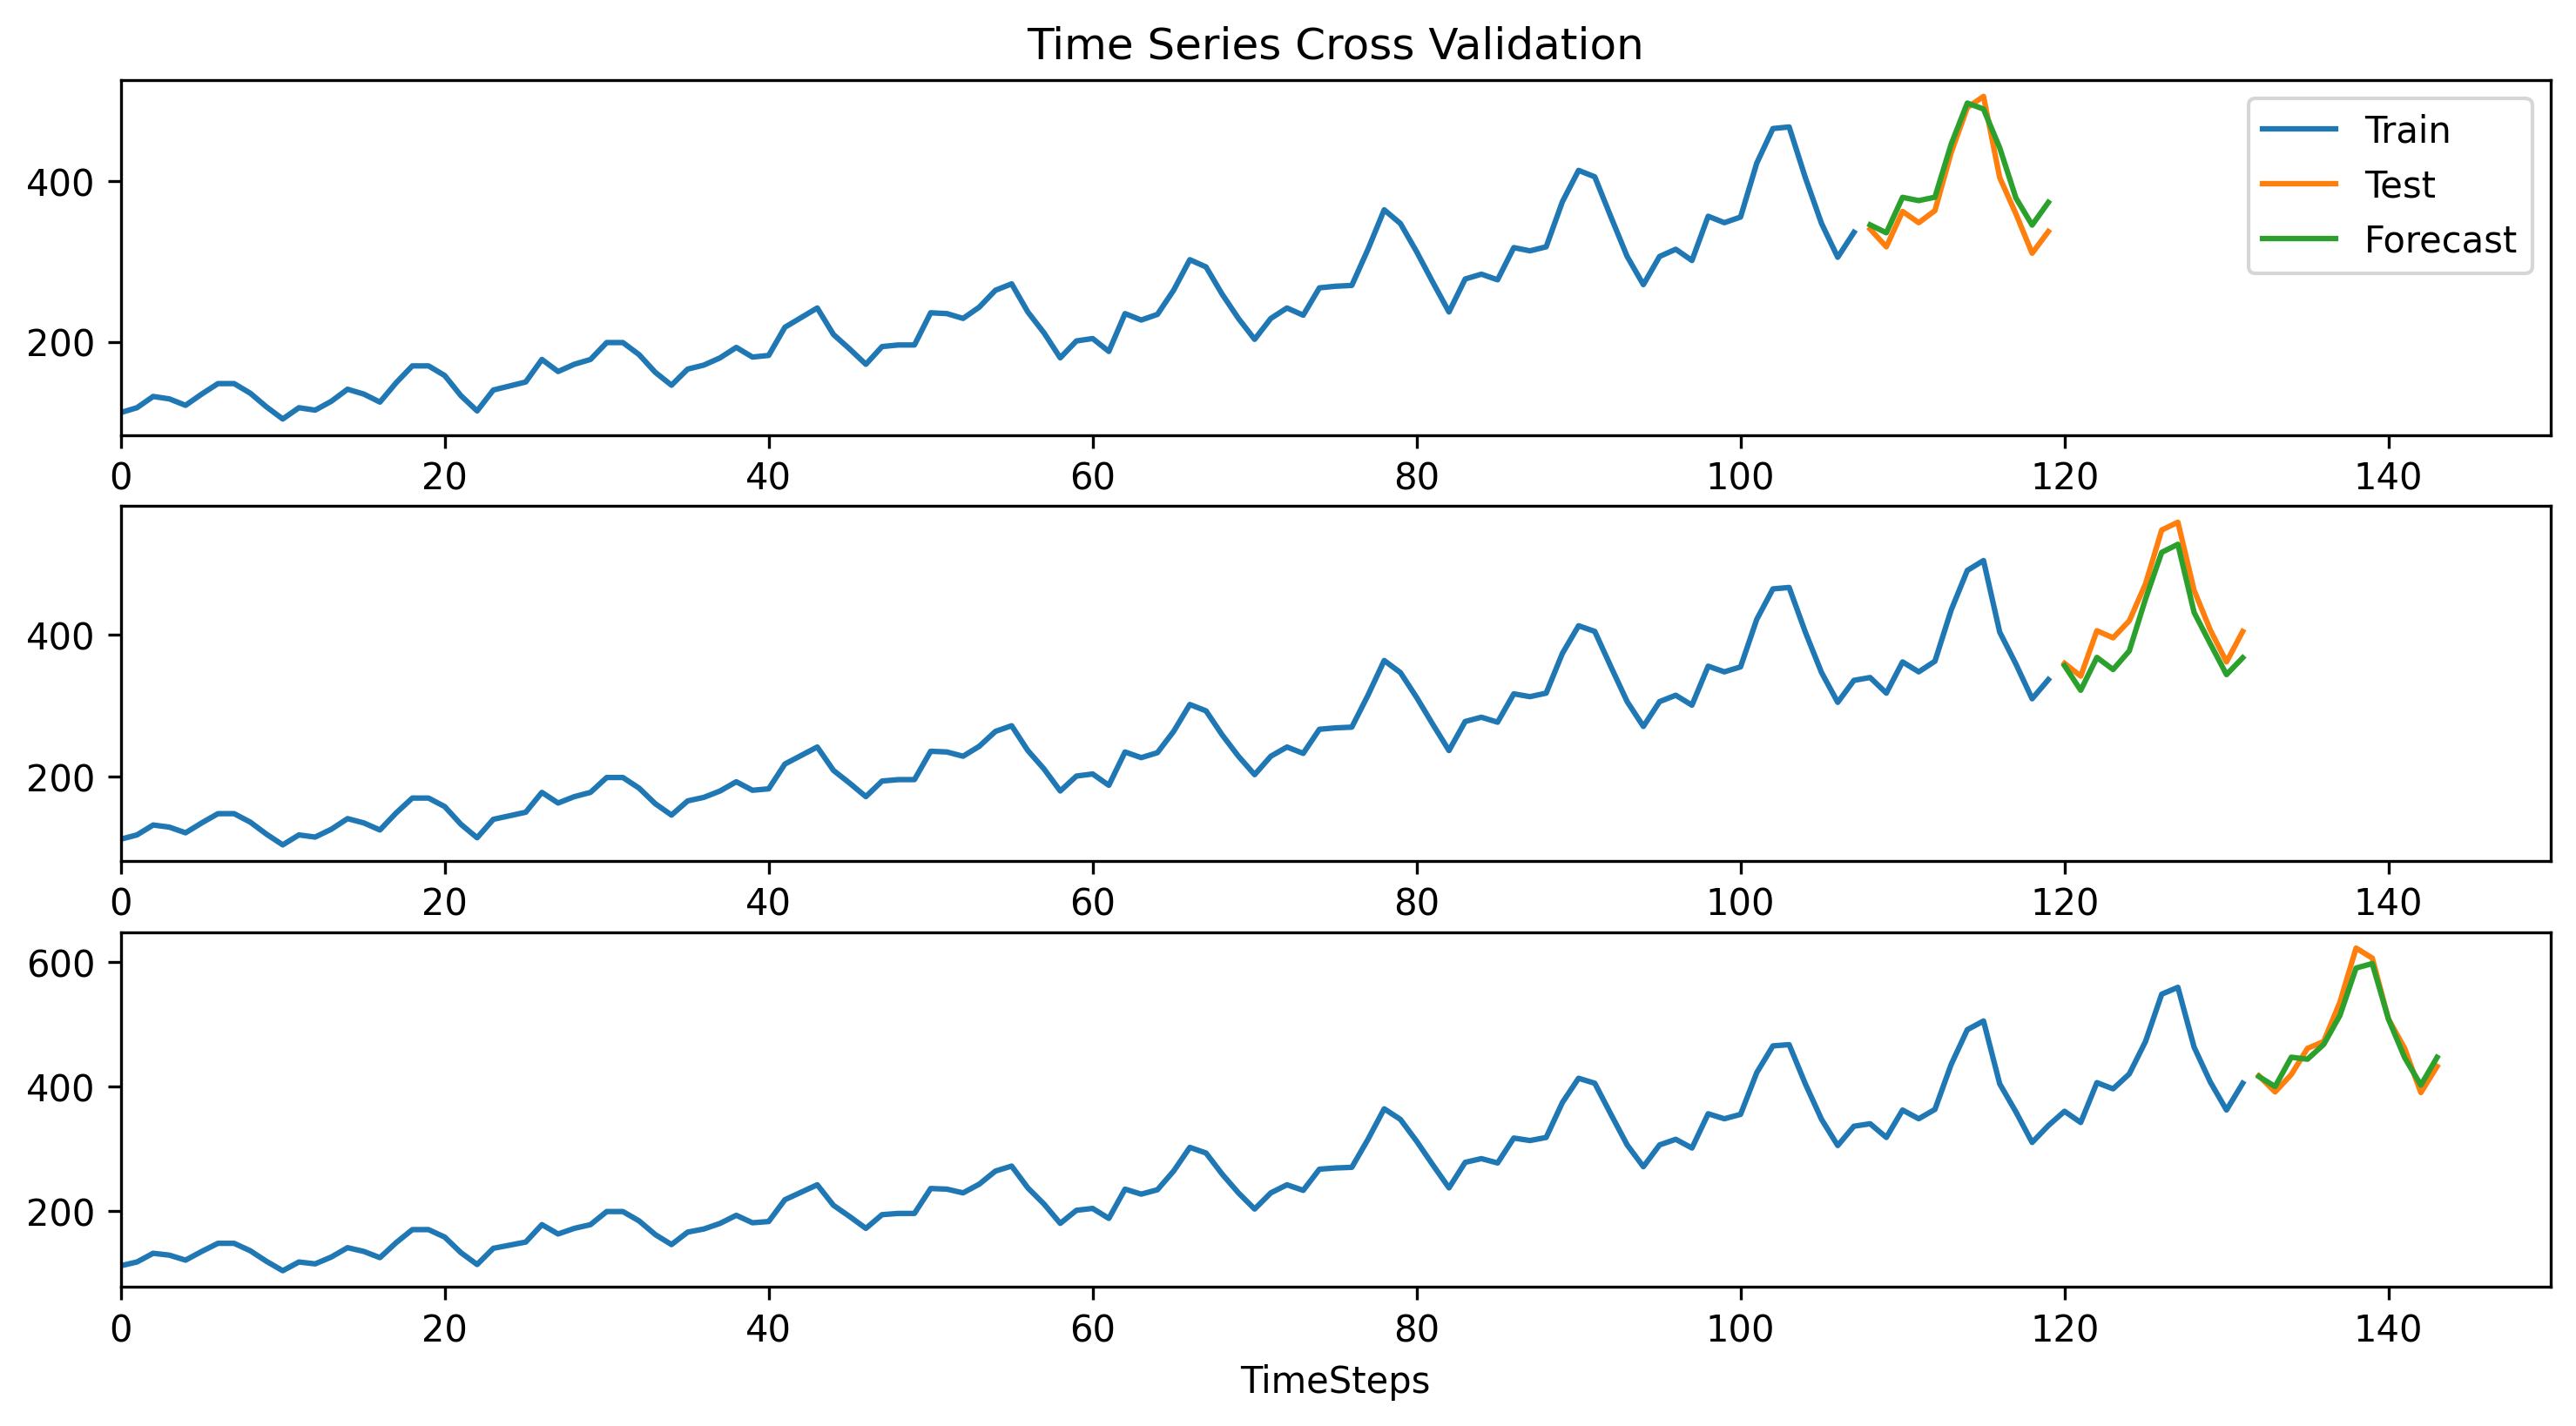
\includegraphics[scale=0.45]{notebooks/Others/img/time_series_cross_validation.png}
    \caption{Time Series Cross-Validation Example}
\end{figure}









\newpage


% ------------------------------------------------------------------------------
% Reference and Cited Works
% ------------------------------------------------------------------------------

%\bibliographystyle{IEEEtran}
%\bibliography{References.bib}

% ------------------------------------------------------------------------------

\end{document}
